\documentclass{beamer}

\mode<presentation> {


\usetheme{default}
% \setbeamertemplate{footline} % To remove the footer line in all slides uncomment this line
\setbeamertemplate{footline}[page number] % To replace the footer line in all slides with a simple slide count uncomment this line
\setbeamertemplate{navigation symbols}{} % To remove the navigation symbols from the bottom of all slides uncomment this line
}

\usepackage{graphicx} % Allows including images
\usepackage{booktabs} % Allows the use of \toprule, \midrule and \bottomrule in tables
\usepackage{verbatim}
\usepackage{multicol}

\title[VE215 RC 6]{VE215 RC 6}
\author{Erdao Liang, Chongye Yang}
\institute[UM-SJTU JI] 
{UM-SJTU JI}
\date{\today}

\begin{document}

\AtBeginSection[ ]
{
\begin{frame}{Overview}
    \tableofcontents[sectionstyle=show/shaded,subsectionstyle=show/shaded/hide]
    % \tableofcontents[sectionstyle=show/shaded,subsectionstyle=show/shaded]
 \end{frame}
}

%%%%%%%%%%%%%%%%%%%%%%%%%%%%%%%%%%%%%%%%%%%%%%%%%%%
% TITLE PAGE
\begin{frame}
\titlepage % Print the title page as the first slide
\end{frame}






%%%%%%%%%%%%%%%%%%%%%%%%%%%%%%%%%%%%%%%%%%%%%%%%%%%
% AC Power Analysis

% \section{AC Power Analysis}

% %%%%%%%%%%%%%%%%%%%%%%%%%%%%%

% \begin{frame}{Instantaneous and Average Power}
% Both $v(t)$ and $i(t)$ here are instantaneous values. \textcolor[rgb]{1,0,0}{(not rms)}
% $$p(t)=v(t) \cdot i(t)$$
% Instantaneous power:
% \begin{equation*}
% \begin{aligned}
% p(t) &= V_{m}I_{m}cos(\omega t + \theta_{v})cos(\omega t + \theta_{i})\\
% &= \dfrac{1}{2}V_{m}I_{m}cos(\theta_{v}-\theta_{i})+\dfrac{1}{2}V_{m}I_{m}cos(2 \omega t + \theta_{v} + \theta_{i})
% \end{aligned}
% \end{equation*}

% \end{frame}

% %%%%%%%%%%%%%%%%%%%%%%%%%%%%%

% \begin{frame}{Average Power}

% General definition:
% $$P = \frac{1}{T}\int_0^Tp(t)dt$$
% For sinusoids,
% $$P=\dfrac{1}{2}V_{m}I_{m} cos(\theta_{v}-\theta_{i})$$
% Represented with phasor $\tilde{V}$ and $\tilde{I}$,
% $$P = \frac12\mathrm{Re}(\tilde{V}\tilde{I^{\color{red}*\color{black}}})$$

% \end{frame}

% %%%%%%%%%%%%%%%%%%%%%%%%%%%%%
% \begin{frame}{Average Power}

% \begin{itemize}
%     \item when $\theta_{v}-\theta_{i}=0$, purely resistive load $R$.
%     $$P = \frac12I_m^2R=\frac12\frac{V_m^2}{R}$$
%     (the second equality not true when $\theta_{v}-\theta_{i}\neq 0$)
    
%     \item when $\lvert \theta_{v}-\theta_{i} \rvert = 90^{\circ}$, purely reactive load $X$. It absorbs no \textcolor[rgb]{1,0,0}{average} power.
%     \item Generally,
%     $$\begin{aligned}
%         P &= \dfrac{1}{2}V_{m}I_{m} cos(\theta_{v}-\theta_{i}) = \dfrac{1}{2}\mathrm{Re}(\tilde{V} \tilde{I}^{*})= \dfrac{1}{2} \mathrm{Re}((\tilde{I}Z)\tilde{I}^{*})\\
%         & = \frac12\mathrm{Re}(I^2R+jI^2X)= \color{red}\dfrac{1}{2} I_{m}^{2}R
%     \end{aligned}$$
%     (Only resistance contributes to the average power absorbance)
% \end{itemize}

% \end{frame}

% %%%%%%%%%%%%%%%%%%%%%%%%%%%%%


% \begin{frame}{Maximum Average Power Transfer}
% \begin{figure}
% \centering
% 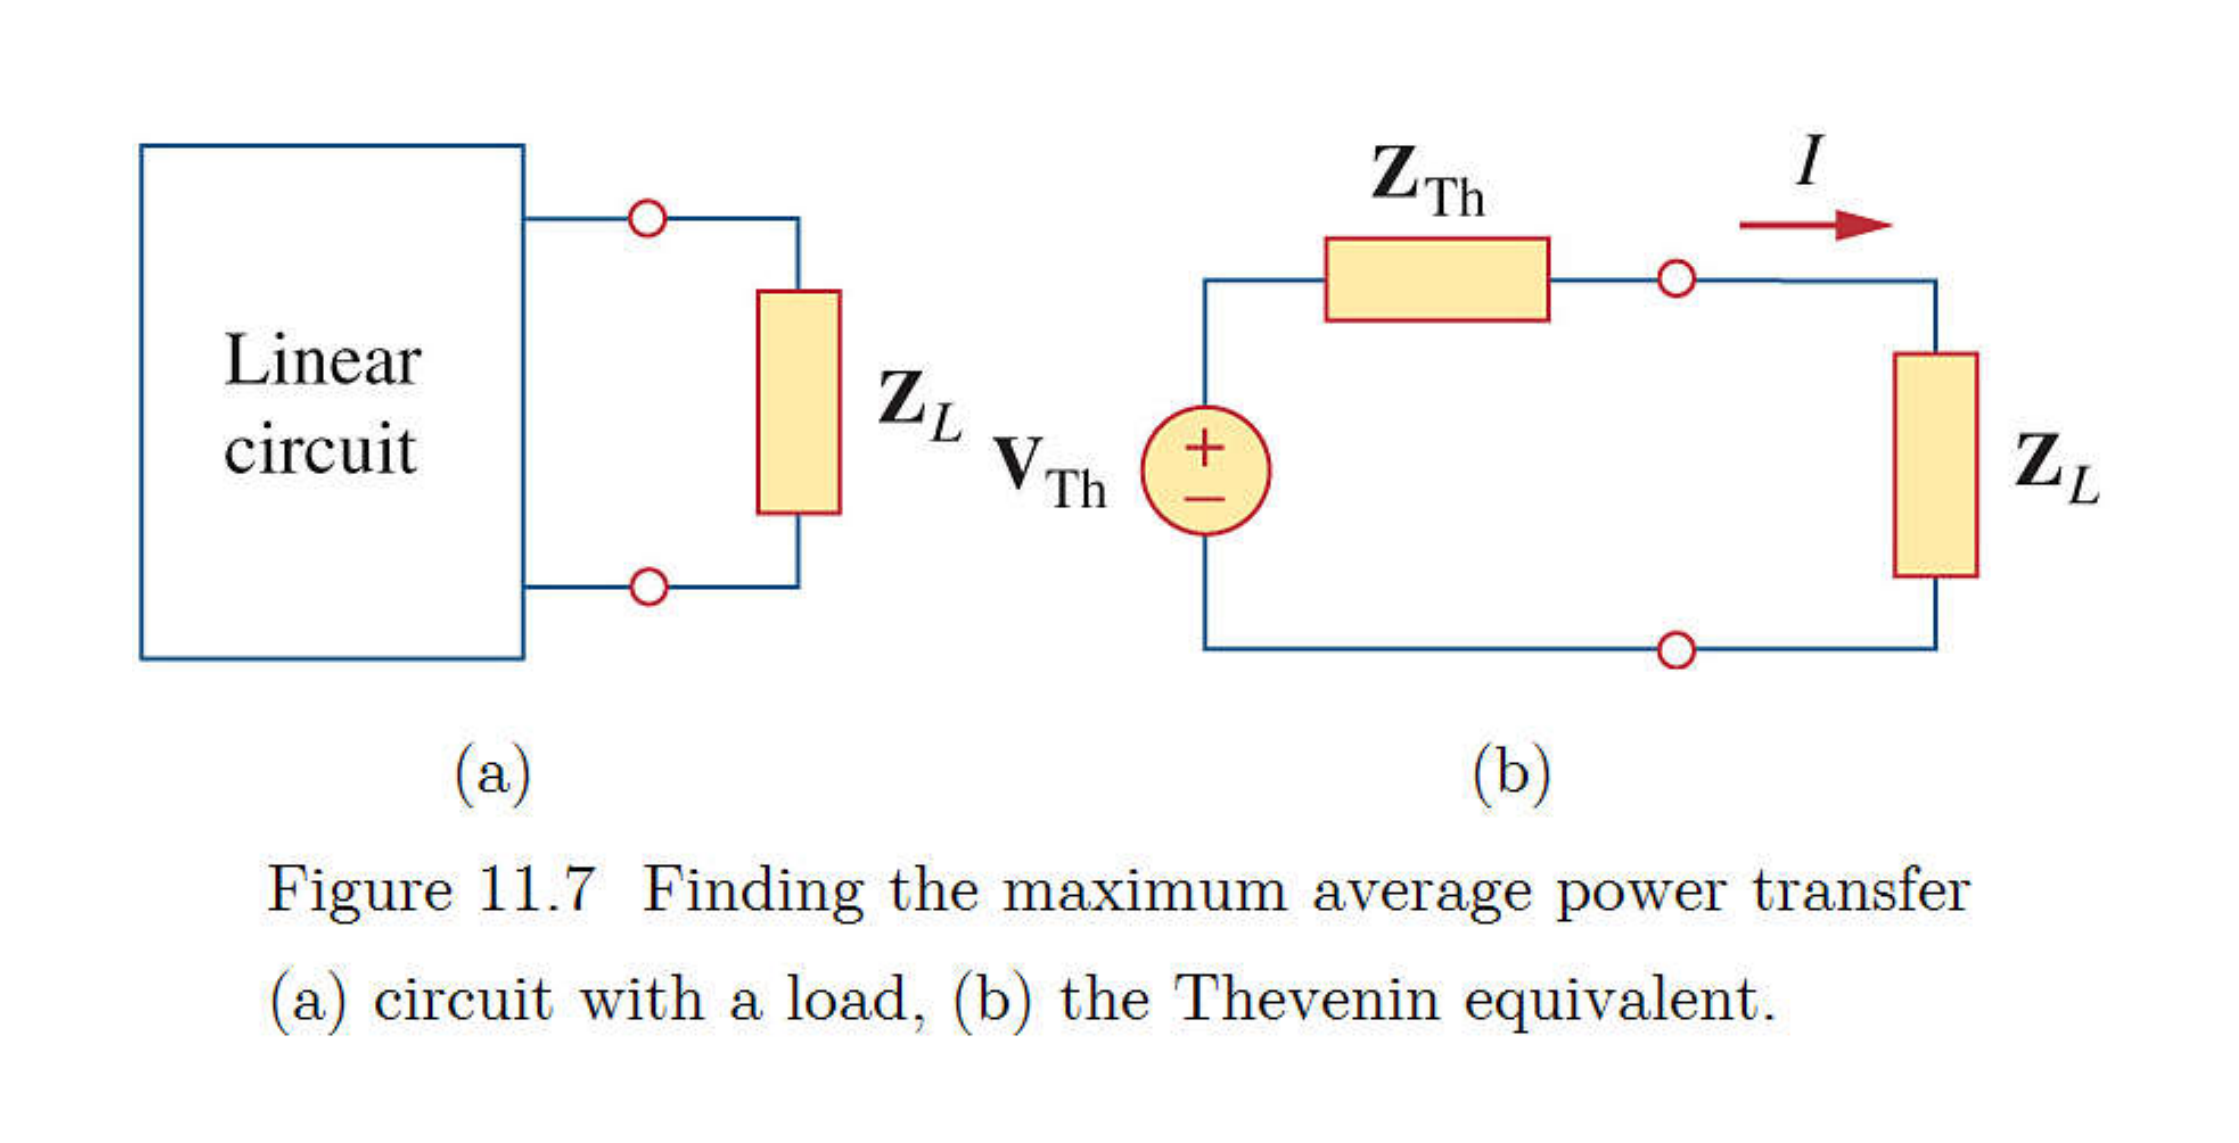
\includegraphics[width=3.5in]{img_ch11/maximum_power.png}
% \end{figure}
% \begin{itemize}
% \item If there is no restriction on $Z_L$,
% $$R_{L}=R_{Th}\ \ \ X_{L}=-X_{Th}\ \ \ P_{max}=\dfrac{\lvert V_{Th }^{2} \rvert}{8R_{Th}}$$
% \item If $Z_L$ is purely resistive,
% $$R_{L}=\sqrt{R_{Th}^{2}+X_{Th}^{2}}$$
% \end{itemize}
% \end{frame}

% %%%%%%%%%%%%%%%%%%%%%%%%%%%%%

% % TODO: motivation and definition
% % TODO:重新排版
% \begin{frame}{Effective or RMS Value}

% Definition: The effective value of a periodic current is the dc current that delivers the same average power to a resistor as the periodic current (similarly for voltage).
% $$I_{eff}^2R = \frac{R}{T}\int_0^Ti^2dt$$

% Effective value = RMS (root mean square) value.


% \begin{equation*}
% \begin{aligned}
% I_{rms} &= \sqrt{\dfrac{1}{T} \int_{0}^{T} i^{2} \mathrm{d} t} = I_{eff} \\
% V_{rms} &= \sqrt{\dfrac{1}{T} \int_{0}^{T} v^{2} \mathrm{d} t} = V_{eff} \\
% \end{aligned}
% \end{equation*}

% \end{frame}

% %%%%%%%%%%%%%%%%%%%%%%%%%%%%%

% \begin{frame}{Effective or RMS Value}

% \begin{itemize}
%     \item Avg power absorbed by a circuit element (generally true):
% $$P = I_{rms}^R=V_{rms}^2\frac{R}{R^2+X^2}$$
% \begin{tiny}
% \begin{center}
%     $P = \dfrac{1}{2}\mathrm{Re}(\tilde{V}\tilde{I}^{*})=\mathrm{Re}(\tilde{V_{rms}}\tilde{I^{*}_{rms}}) = \dfrac{1}{2} I_{m}^{2} R=I_{rms}^{2}R = \dfrac{1}{2} V_{m}^{2} \mathrm{Re} (\dfrac{1}{Z^{*}}) = V_{rms}^{2} \dfrac{R}{R^{2}+X^{2}}$
% \end{center}

% \hspace{0.1mm}
% \end{tiny}
%     \item RMS value for a sinusoid \color{red} sinusoid\color{black}: 
% \begin{equation*}
% I_{rms} = \dfrac{I_{m}}{\sqrt{2}} \qquad
% V_{rms} = \dfrac{V_{m}}{\sqrt{2}}
% \end{equation*}

%     \item Average power absorbed by an element in a \color{red}sinusoidal \color{black}  circuit:

%     $$P = V_{rms}I_{rms}\cos(\theta_v-\theta_i)$$
    
% \end{itemize}

% \end{frame}

% \begin{frame}{Effective or RMS Value}

% \textbf{Caution: from now on, unless specified, all values will be assumed to be RMS values.}
% \end{frame}

% %%%%%%%%%%%%%%%%%%%%%%%%%%%%%


% \begin{frame}{Complex Power}

% We define this ``complex power" that includes all the information.

% $$\begin{aligned}
%     \text{Complex Power}&=\tilde{S}=\tilde{V_{rms}}\tilde{I_{rms}^{\color{red}*\color{black}}} = \lvert I_{rms}\rvert \lvert V_{rms} \rvert \angle (\theta_{v}\color{red}-\color{black}\theta_{i})\\
%     &=\lvert S \rvert \angle (\theta_{v}\color{red}-\color{black}\theta_{i}) \text{ (polar form)}\\
%     &= P+jQ \text{ (rectangular form)}
% \end{aligned}$$

% \begin{table}[]
%     \centering
%     \begin{tabular}{cccc}
%         \toprule
%         Value & Name & Meaning & Unit \\
%         \midrule
%         $\vert S\vert$ & Apparent power & Magnitude of $\tilde{S}$ & VA \\
%         $\cos(\theta_v-\theta_i)$ & Power factor & Cosine of angle of $\tilde{S}$  & / \\ 
%         $P$ & Real power & Real part of $\tilde{S}$ & W \\
%         $Q$ & Complex power & Imaginary part of $\tilde{S}$ & VAR  \\
%         \bottomrule
%     \end{tabular}
% \end{table}


% \end{frame}

% %%%%%%%%%%%%%%%%%%%%%%%%%%%%%
% \begin{frame}{Complex Power}

% \begin{itemize}
%     \item Complex power
%     \begin{center}
%         $
%         \tilde{S}=\tilde{V_{rms}}\tilde{I_{rms}^{\color{red}*\color{black}}} = \lvert I_{rms}\rvert \lvert V_{rms} \rvert \angle (\theta_{v}\color{red}-\color{black}\theta_{i}) =\lvert S \rvert \angle (\theta_{v}\color{red}-\color{black}\theta_{i}) = P+jQ
%         $
%         \hspace{0.1mm}
%         $
%         \tilde{S} = {\vert I_{rms} \vert}^2Z = \frac{{\vert V_{rms}\vert}^2}{Z^{\color{red}*\color{black}}}
%         $
%     \end{center}
        
%     \item Apparent power
%      $$
%      \lvert S \rvert=  \vert V_{rms}\vert\vert I_{rms}\vert =\lvert I_{rms} \rvert ^{2} \lvert Z \rvert = \sqrt{P^2+Q^2}
%      $$

%     \item Real power
%     $$P = \mathrm{Re}(\tilde{S}) = \vert S\vert \cos(\theta_v-\theta_i) = \lvert I_{rms} \rvert ^{2} R$$
%     \item Complex power
%     $$Q = \mathrm{Im}(\tilde{S}) = \vert S\vert \sin(\theta_v-\theta_i) = \lvert I_{rms} \rvert ^{2} X$$
%     \item Power factor
%     $$
%     \text{pf} = \frac{P}{\vert S\vert} = \cos(\theta_v-\theta_i)
%     $$
% \end{itemize}

% \end{frame}

% \begin{frame}{Complex Power}
%     Power factor
%     $
%     \text{pf} = \frac{P}{\vert S\vert} = \cos(\theta_v-\theta_i)
%     $:
%     \begin{itemize}
%         \item $\theta_v - \theta_i < 0$: leading pf
%         \item $\theta_v - \theta_i >0$: lagging pf
%     \end{itemize}
    
%     Since $\cos (\theta_v - \theta_i) = \cos (\theta_i - \theta_v)$, the pf value only tells part of the story. Every time you are asked for a power factor, \color{red} you must declare whether it is leading or lagging\color{black}.
% \end{frame}

% %%%%%%%%%%%%%%%%%%%%%%%%%%%%%

% \begin{frame}{Complex Power}

% We can use the sign of pf angle or $Q$ to identify the property of the circuit and the loads:

% \begin{table}[]
%     \centering
%     \begin{tabular}{c|c|c|c}
%         \hline
%         &(1)&(2)&(3)\\
%         \hline
%         pf Angle & $\theta_v-\theta_i=0$ & $\theta_v-\theta_i<0$ & $\theta_v-\theta_i>0$  \\ 
%         Sign of $Q$ &$Q = 0$ & $Q<0$ & $Q>0$ \\
%         \hline
%         &Unity pf & Leading pf & Lagging pf \\
%         Properties &$I$, $V$ in phase & $I$ leads $V$ & $I$ lags $V$ \\
%         &$X = 0$ & $X<0$& $X>0$\\
%         &Resistive loads&Capacitive loads&Inductive loads\\
%         \hline
        
%     \end{tabular}
% \end{table}
    
% \end{frame}

% %%%%%%%%%%%%%%%%%%%%%%%%%%%%%
% \begin{frame}{Complex Power}

% \begin{multicols}{2}
%         \sectiont{}
% \begin{figure}
%     \centering
%     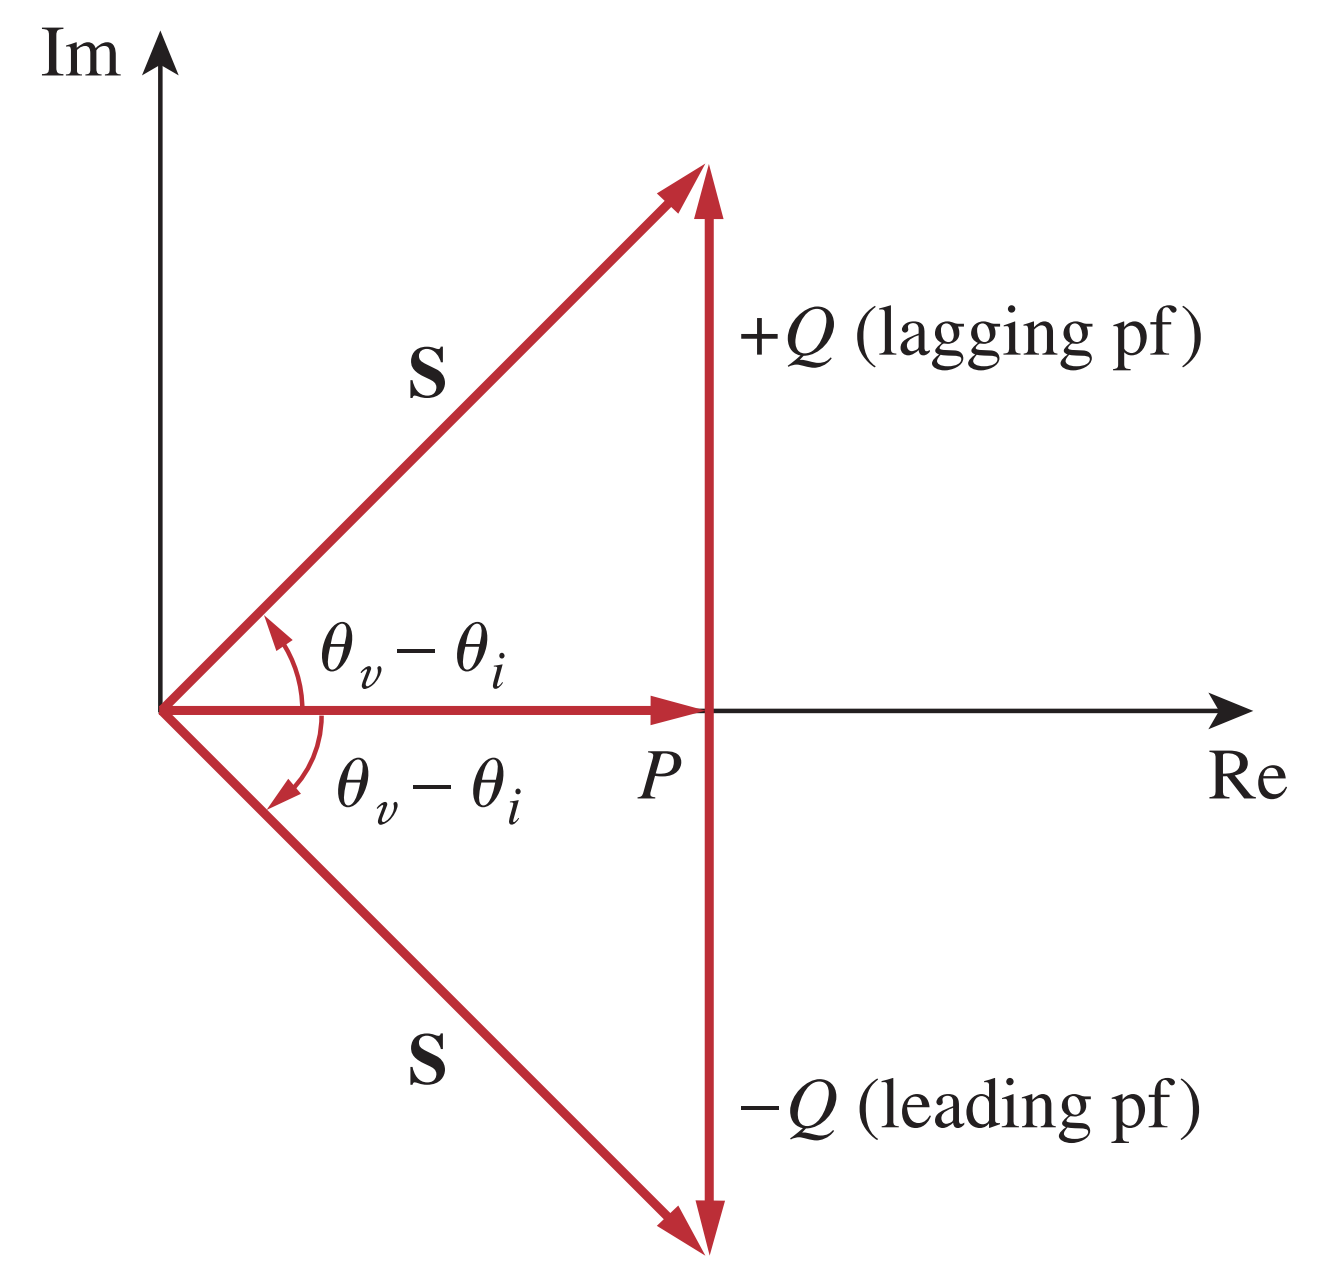
\includegraphics[width=0.48\textwidth]{img_ch11/power triangle.png}
% \end{figure}
%         \sectiont{}
% And observe that the power factor angle is equal to the angle of the impedance of that part of the circuit.
% \begin{figure}
% \centering
% 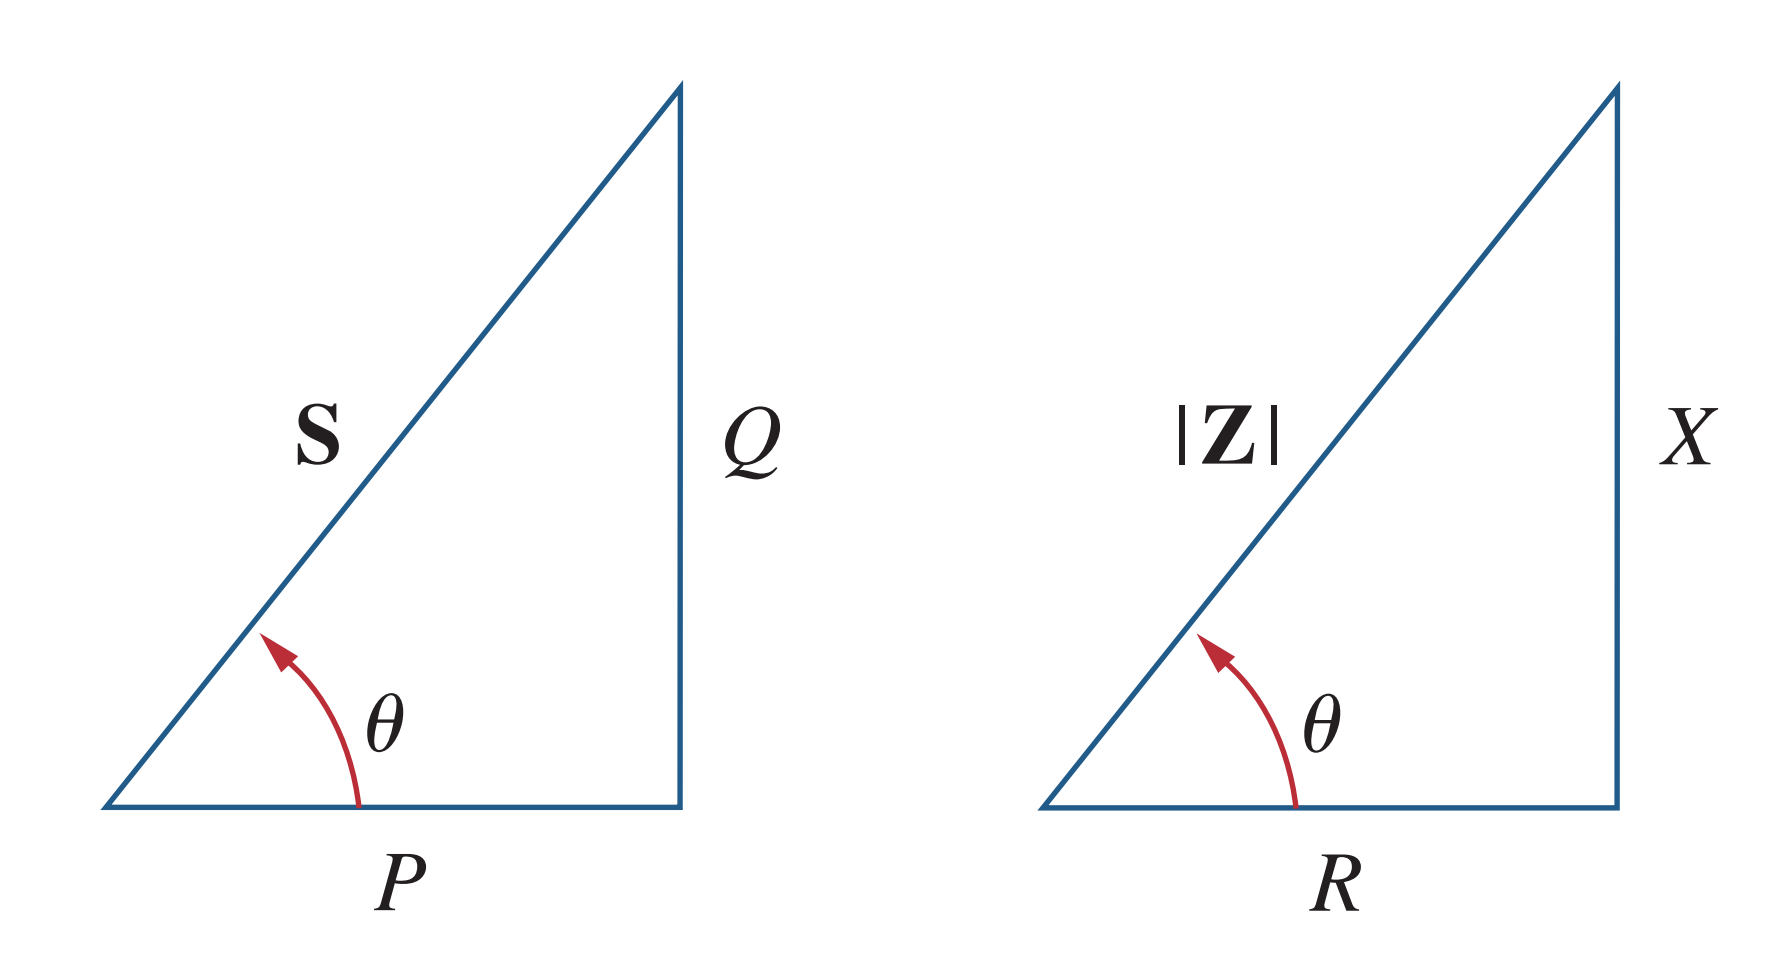
\includegraphics[width=0.48\textwidth]{img_ch11/pf.png}
% \end{figure}
        
        
% \end{multicols}
% \end{frame}



% %%%%%%%%%%%%%%%%%%%%%%%%%%%%%
% \begin{frame}{Exercise 1}
% \textbf{Question}:
% \newline
% A series-connected load draws a current $i(t)=4cos(100\pi t+10^{\circ}) A$ when the applied voltage is $v(t)=120cos(100\pi t-20^{\circ})V$. Find the apparent power and the power factor of the load. Determine the element values that form the series-connected load.
% \end{frame}

% %%%%%%%%%%%%%%%%%%%%%%%%%%%%%
% \begin{frame}{Exercise 1}
% \begin{figure}
% \centering
% 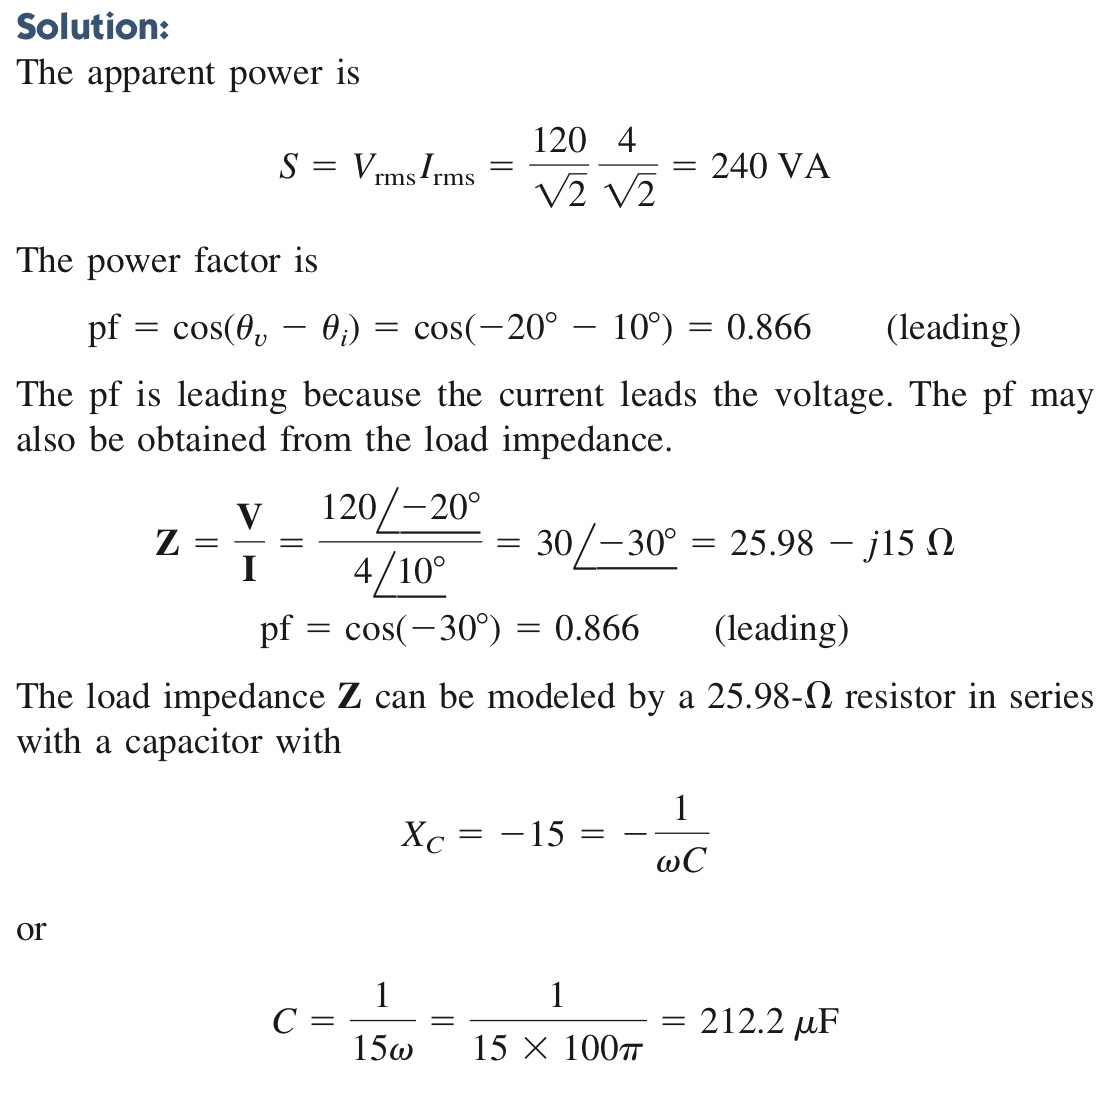
\includegraphics[width=3in]{img_ch11/s1.jpg}
% \end{figure}  
% \end{frame}

% %%%%%%%%%%%%%%%%%%%%%%%%%%%%%


% \begin{frame}{Power Factor Correction}
% \begin{itemize}
%     \item Goal: increase the pf of a load $\rightarrow$ make it less inductive $\rightarrow$ reduce energy loss

%     \item Solution: add a capacitor in parallel to the load

%     \begin{figure}
%         \centering
%         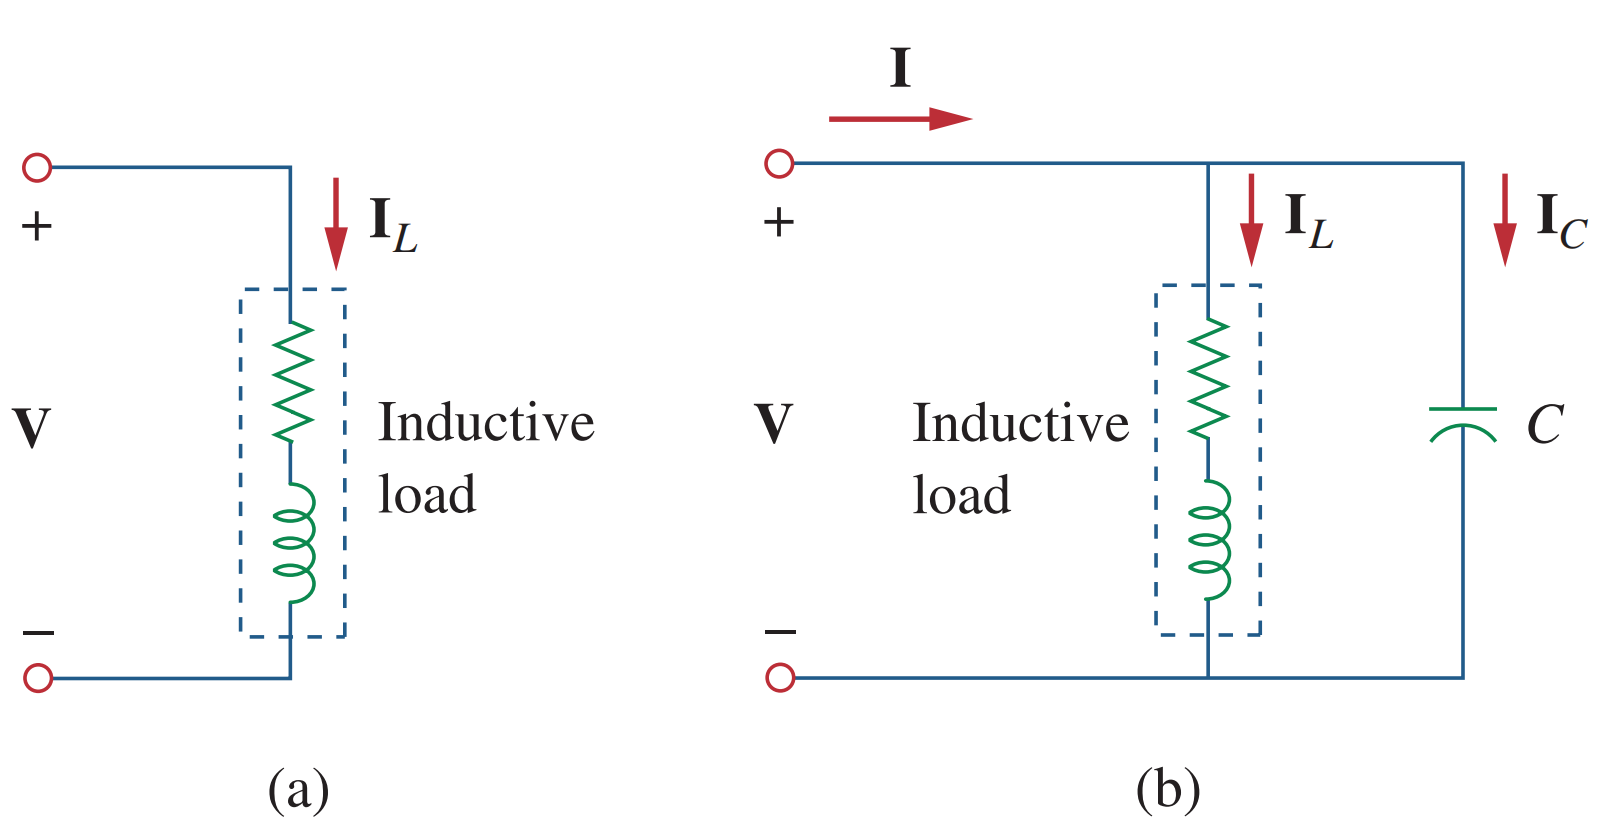
\includegraphics[width=0.7\textwidth]{img_ch11/add capacitor.png}
%     \end{figure}
    
% \end{itemize}

% \end{frame}

% %%%%%%%%%%%%%%%%%%%%%%%%%%%%%
% \begin{frame}{Power Factor Correction}

% Goal: increase the pf from $\cos \theta_1$ to $\cos \theta_2$.
% \begin{multicols}{2}
% \sectiont{}
% \begin{figure}
%     \centering
%     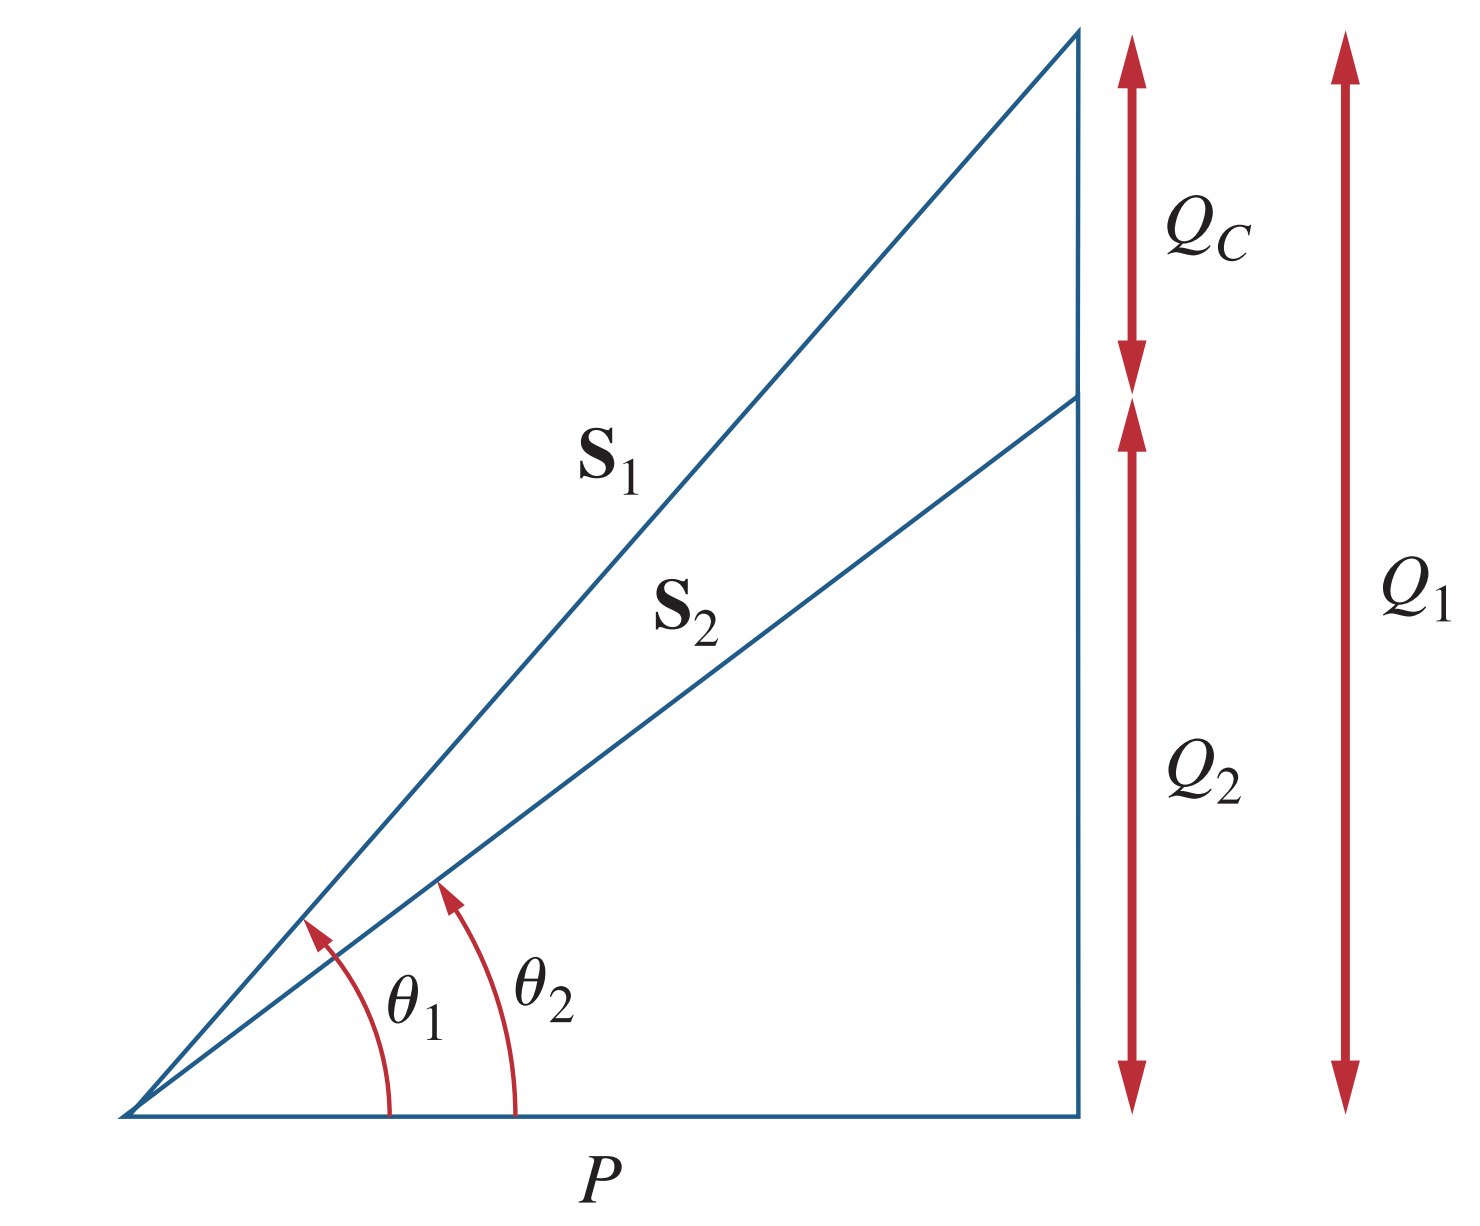
\includegraphics[width=0.4\textwidth]{img_ch11/triangle2.png}
% \end{figure}
% \sectiont{}
% Initial:

% $P = \vert S_1\vert \cos \theta_1$

% $Q_1 = \vert Q_1\vert \sin \theta_1= P \tan \theta_1$

% \vspace{0.3cm}
% The ``after" we expect:

% $P = \vert S_2\vert \cos \theta_2$

% $Q_2 = \vert Q_2\vert \sin \theta_2= P \tan \theta_2$
        
% \end{multicols}

% Since $Q_c(=Q_1-Q_2)= \frac{V_{rms}^2}{X_c}$, then the value of the required capacitance $C$ is 
% $$C = \frac{Q_C}{\omega V_{rms}^2} = \frac{Q_2-Q_1}{\omega V_{rms}^2} = \color{red}\frac{P(\tan \theta_1 - \tan \theta_2)}{\omega V_{rms}^2}$$
% \end{frame}


% %%%%%%%%%%%%%%%%%%%%%%%%%%%%%
% \begin{frame}{Exercise 2}
% \textbf{Question}:
% \newline
% When connected to a 120-V (rms), 60-Hz power line, a load absorbs 4 kW at a lagging power factor of 0.8. Find the value of capacitance necessary to raise the pf to 0.95.
% \end{frame}

% %%%%%%%%%%%%%%%%%%%%%%%%%%%%%
% \begin{frame}{Exercise 2}
% \textbf{Question}:
% \newline
% When connected to a 120-V (rms), 60-Hz power line, a load absorbs 4 kW at a lagging power factor of 0.8. Find the value of capacitance necessary to raise the pf to 0.95.
% \newline
% \newline
% \textbf{Formula}: $C=\dfrac{P  \tan(\theta_{1}-\theta_{2})}{\omega \cdot V_{rms}^{2}}$
% \newline
% \newline
% \textbf{Answer}: 310.5 $\mu$F
% \end{frame}

%%%%%%%%%%%%%%%%%%%%%%%%%%%%%%%%%%%%%%%%%%%%%%%%%%%
% Three Phase Circuit

\section{Three-Phase Circuits}

\begin{frame}{Ployphase}
    Sources operate at the same frequency but different phases. \\
    For example, the figure below shows a three-phase four-wire system:
    \begin{figure}[H]
        \centering
        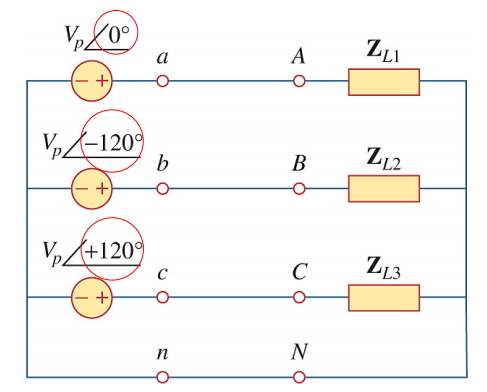
\includegraphics[scale = 0.7]{C12/1.png}
        \label{fig:enter-label}
    \end{figure}
\end{frame}

\begin{frame}{Three-Phase Circuits}
    Three-Phase Voltage sources
    \begin{itemize}
        \item Type: Y-connected, $\Delta$-connected
        \item Balanced: $\textbf{V}_{an}+\textbf{V}_{bn}+\textbf{V}_{cn} = 0$\\
            $\ \ \ \ \ \ \ \ \ \ \ \ \ |\textbf{V}_{an}|=|\textbf{V}_{bn}|=|\textbf{V}_{cn}|$
        \item Phase sequences: abc/positive, acb/negative.
    \end{itemize}
\end{frame}

\begin{frame}{Types}
    \begin{figure}[H]
        \centering
        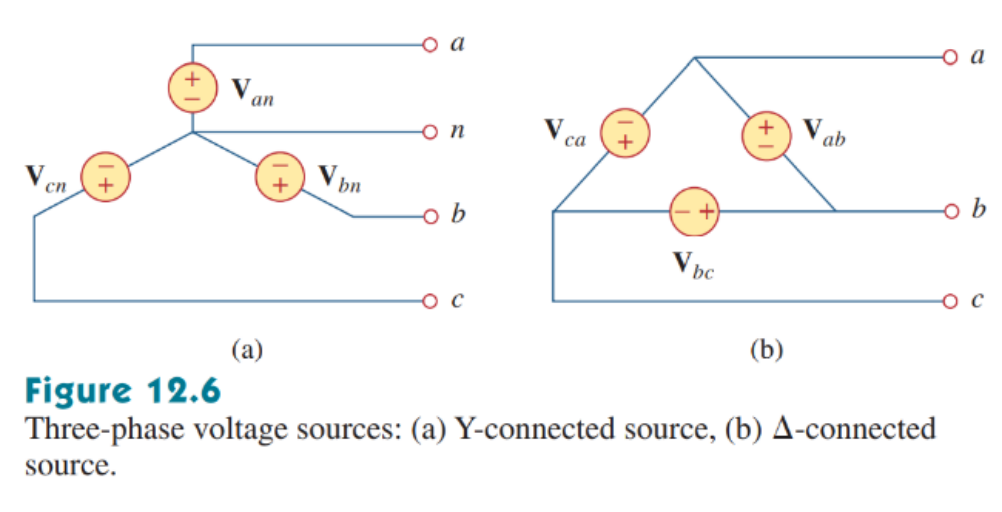
\includegraphics[scale = 0.5]{C12/2.png}
        \label{fig:enter-label}
    \end{figure}
\end{frame}

\begin{frame}{Phase sequences}
    \begin{figure}[H]
        \centering
        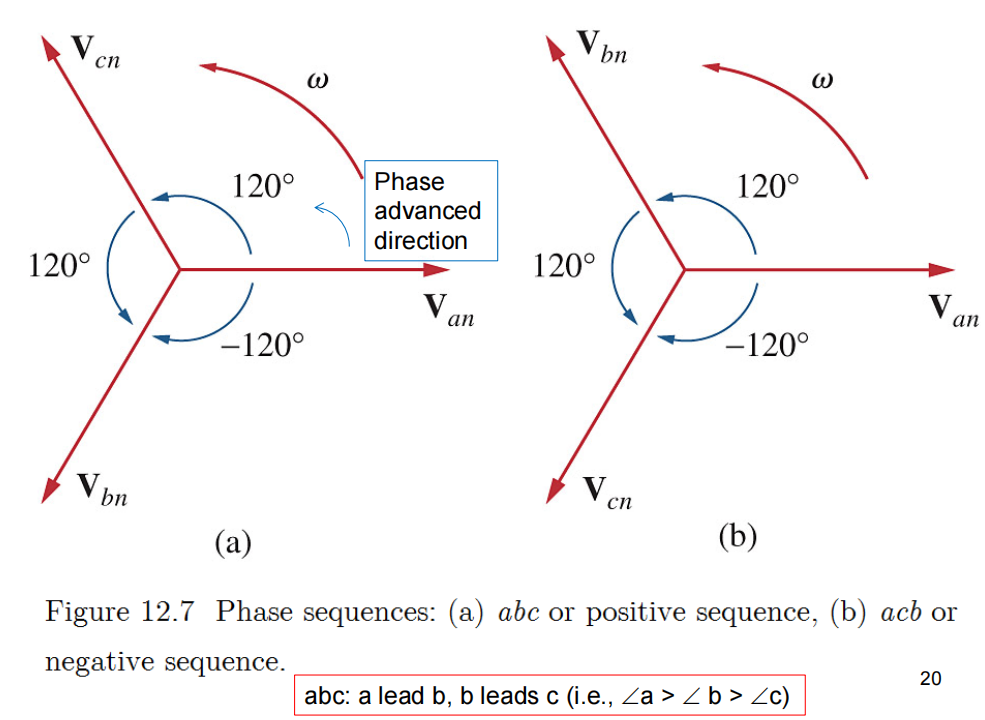
\includegraphics[scale = 0.5]{C12/3.png}
        \label{fig:enter-label}
    \end{figure}
\end{frame}

\begin{frame}{Three-Phase Loads}
    \begin{itemize}
        \item Type: Y-connected, $\Delta$-connected
        \item Balanced: $\textbf{Z}_1=\textbf{Z}_2=\textbf{Z}_3=\textbf{Z}_Y$ \\
        $\ \ \ \ \ \ \ \ \ \ \ \ \ \ \textbf{Z}_a=\textbf{Z}_b=\textbf{Z}_c=\textbf{Z}_{\Delta}$\\
        $\ \ \ \ \ \ \ \ \ \ \ \ \ \ \ \ \ \ \ \ \ \textbf{Z}_{\Delta}=3\textbf{Z}_Y$
    \end{itemize}
    \begin{figure}[H]
        \centering
        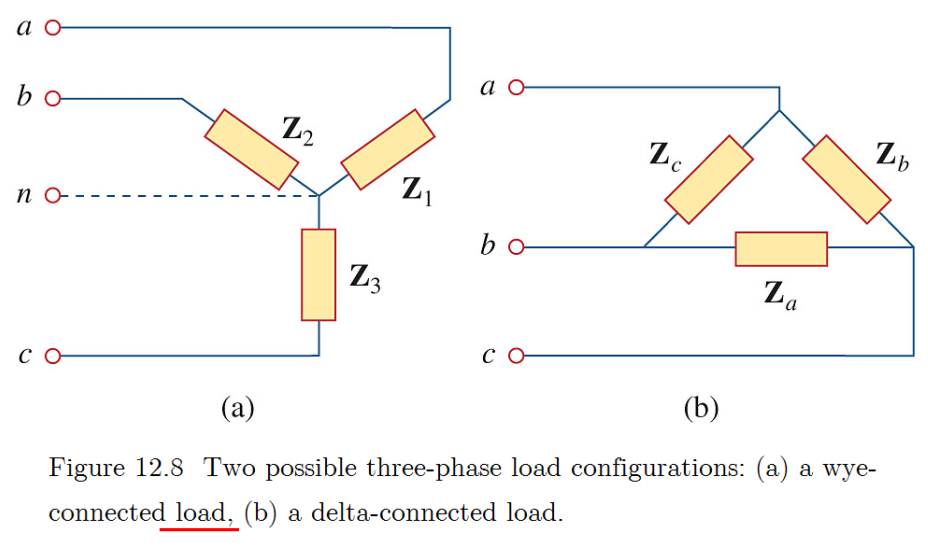
\includegraphics[scale = 0.4]{C12/4.png}
        \label{fig:enter-label}
    \end{figure}
\end{frame}

\begin{frame}{Three-Phase circuits}
    Connect types
    \begin{itemize}
        \item Y-Y
        \item Y-$\Delta$
        \item $\Delta$-Y
        \item $\Delta$-$\Delta$
    \end{itemize}
    Some terms
    \begin{itemize}
        \item Line: conductors connecting sources and loads.
        \item Line voltages: the voltage between any two lines.
        \item Line currents: the current passing along each line.
        \item Phase: connected between any pair of line terminals \textcolor{red}{(an element)}.
        \item Phase voltages: the voltage across any phase.
        \item Phase currents: the current passing through any phase.
    \end{itemize}
\end{frame}

\begin{frame}{Y-Y Connection}
    \begin{figure}[H]
        \centering
        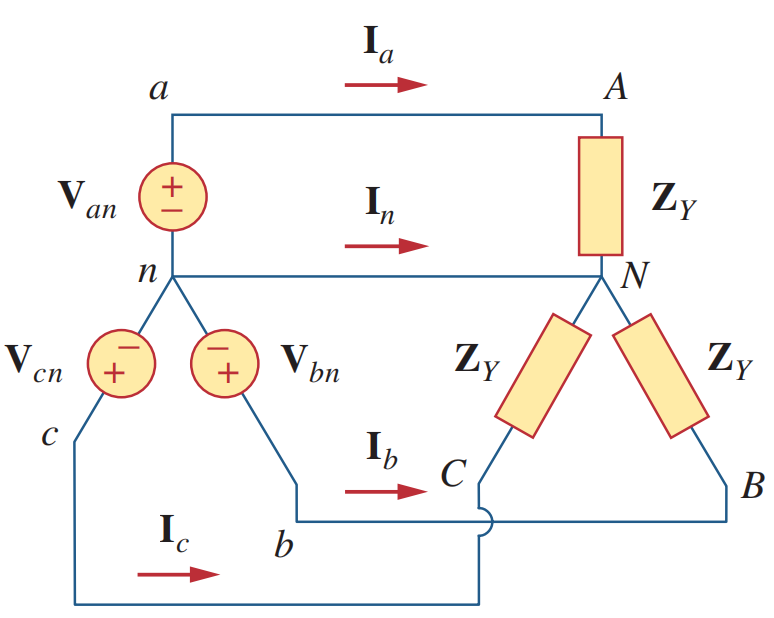
\includegraphics[scale = 0.4]{C12/yy.png}
        \label{fig:enter-label}
    \end{figure}
    \begin{figure}[H]
        \centering
        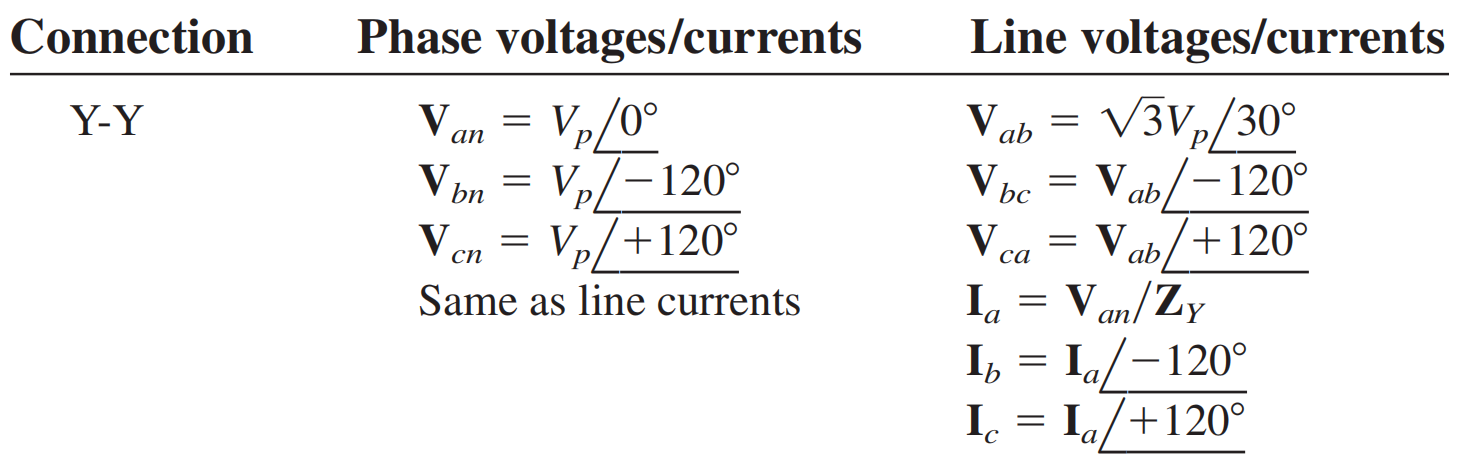
\includegraphics[scale = 0.3]{C12/yy1.png}
        \label{fig:enter-label}
    \end{figure}
\end{frame}

\begin{frame}{Y-$\Delta$ Connection}
    \begin{figure}[H]
        \centering
        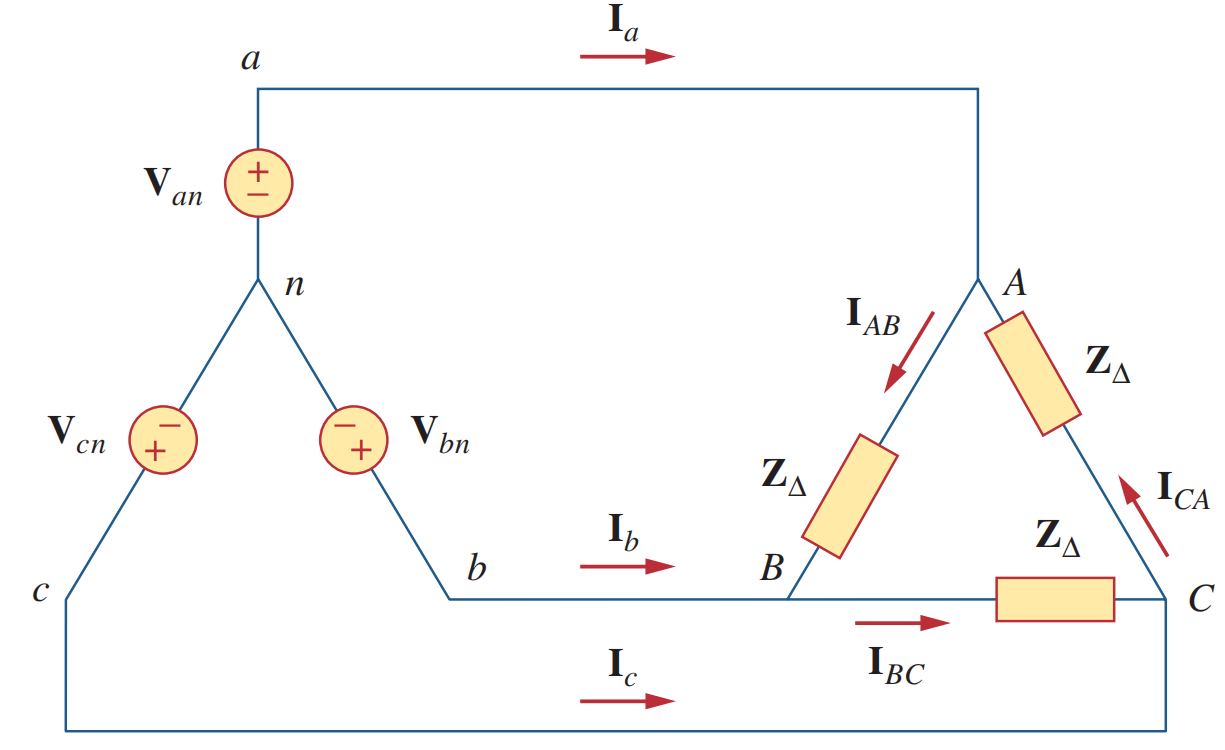
\includegraphics[scale = 0.35]{C12/yd.png}
        \label{fig:enter-label}
    \end{figure}
    \begin{figure}[H]
        \centering
        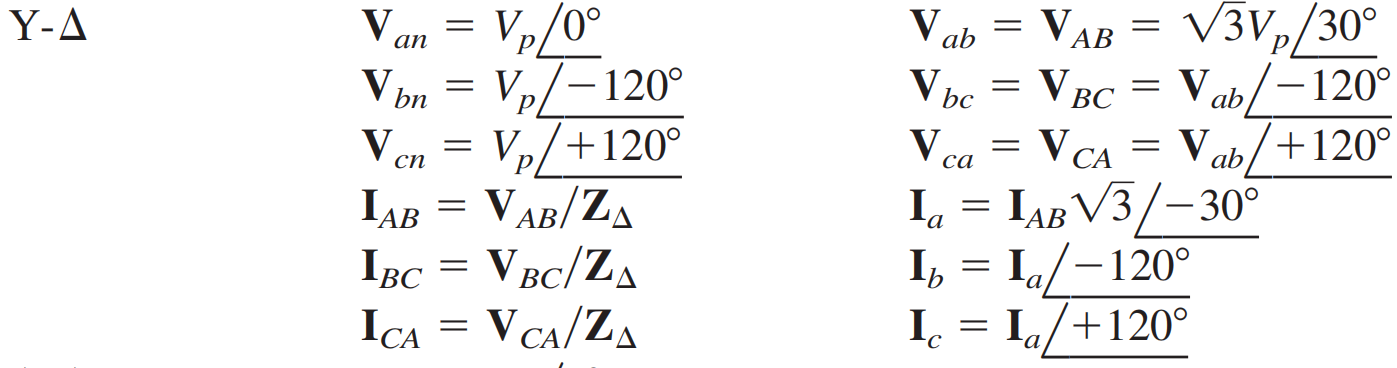
\includegraphics[scale = 0.35]{C12/yd1.png}
        \label{fig:enter-label}
    \end{figure}
\end{frame}

\begin{frame}{$\Delta$-$\Delta$ Connection}
    \begin{figure}[H]
        \centering
        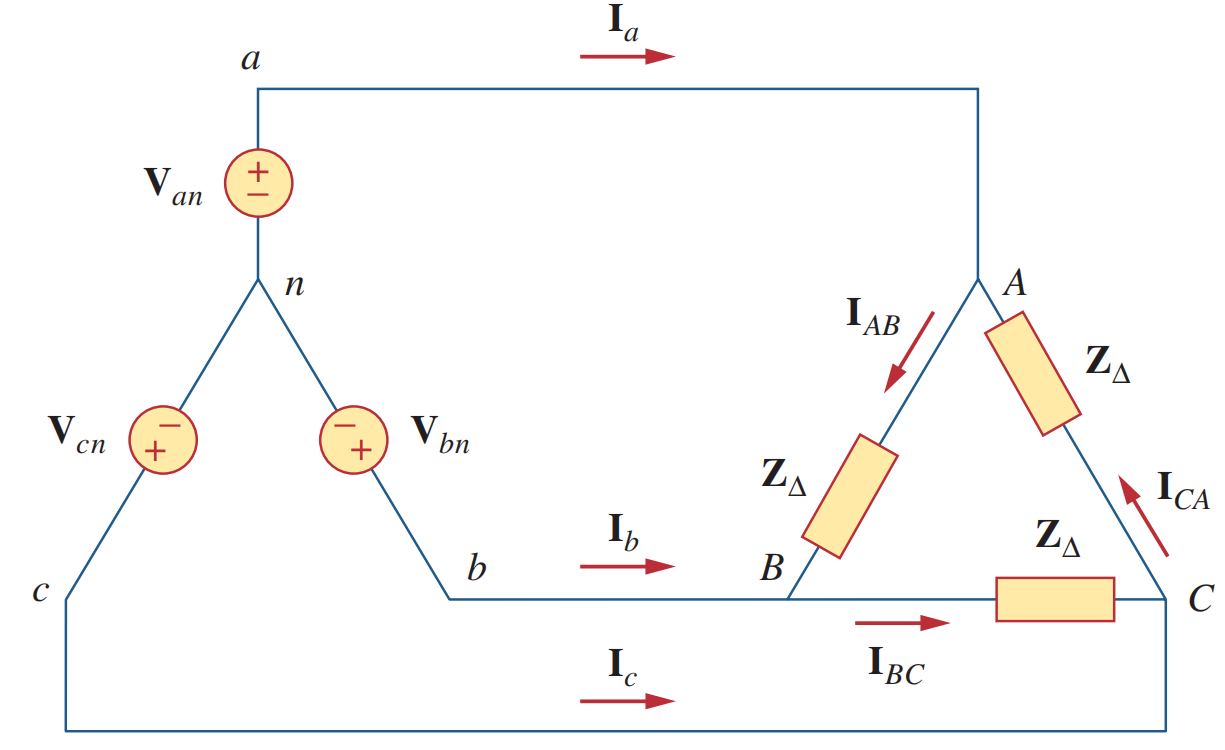
\includegraphics[scale = 0.35]{C12/yd.png}
        \label{fig:enter-label}
    \end{figure}
    \begin{figure}[H]
        \centering
        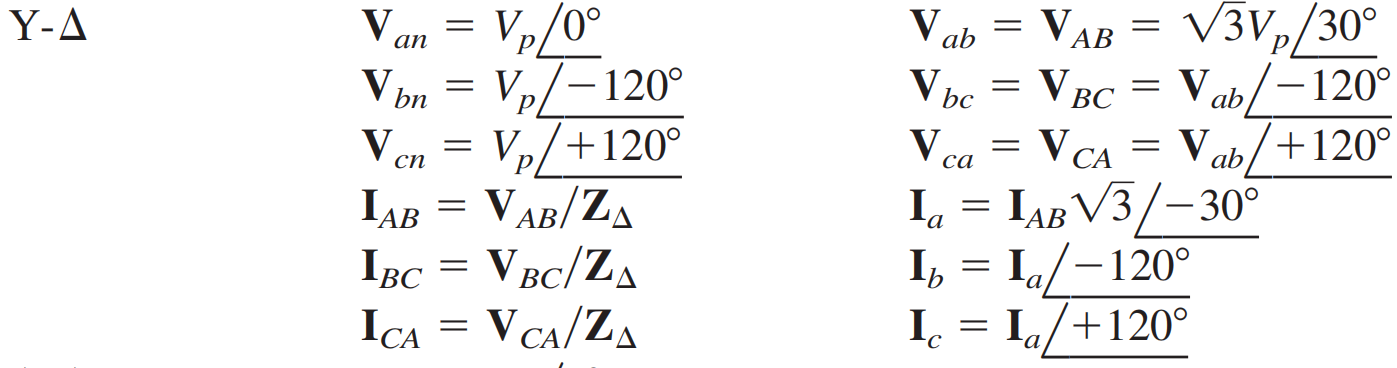
\includegraphics[scale = 0.3]{C12/yd1.png}
        \label{fig:enter-label}
    \end{figure}
\end{frame}

\begin{frame}{$\Delta$-Y Connection}
    \begin{figure}[H]
        \centering
        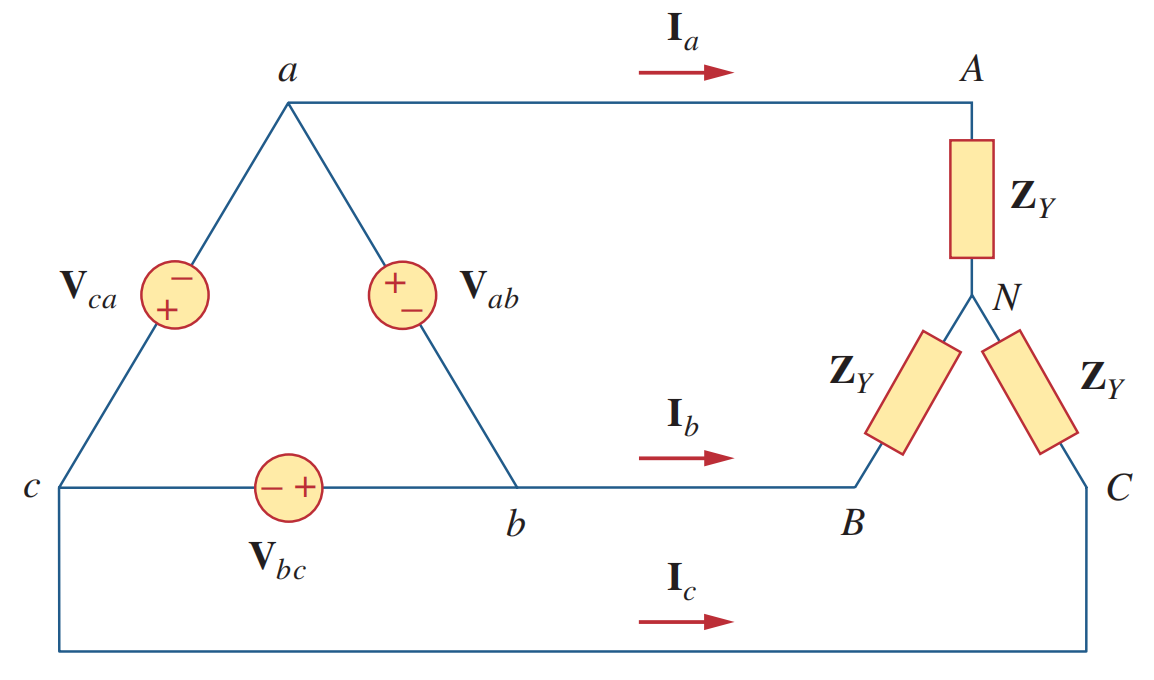
\includegraphics[scale = 0.35]{C12/dy.png}
        \label{fig:enter-label}
    \end{figure}
    \begin{figure}[H]
        \centering
        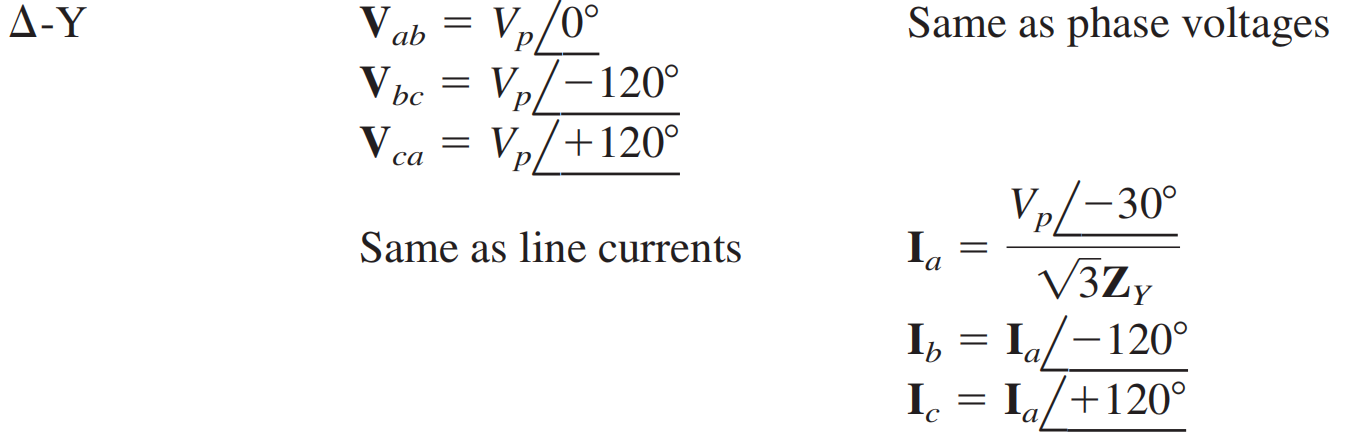
\includegraphics[scale = 0.3]{C12/dy1.png}
        \label{fig:enter-label}
    \end{figure}
\end{frame}

\begin{frame}{Power}
    \begin{itemize}
        \item Instantaneous power: $p=3|\textbf{V}_p||\textbf{I}_p|\cos \theta=\sqrt{3}|\textbf{V}_L||\textbf{V}_L|\cos \theta$
            \begin{itemize}
                \item Y-load: $\ |\textbf{I}_L|=|\textbf{I}_p|\ \ \ \ \ \ \ |\textbf{V}_L|=\sqrt{3}|\textbf{V}_p|$ 
                \item $\Delta$-Load: $|\textbf{I}_L|=\sqrt{3}|\textbf{I}_p|\ \ \ |\textbf{V}_L|=|\textbf{V}_p|$
            \end{itemize}
        \item Average power: 
            \begin{itemize}
                \item Total: $P=3|\textbf{V}_p||\textbf{I}_p|\cos \theta = \sqrt{3}|\textbf{V}_L||\textbf{I}_L|\cos \theta$
                \item Per phase: $P_p=|\textbf{V}_p||\textbf{I}_p|\cos \theta$
            \end{itemize}
        \item Complex power:
            \begin{itemize}
                \item Total: $S=3\textbf{V}_p \textbf{I}_p^{*}=3|\textbf{I}_p|^2 \textbf{Z}_p$
                \item Per phase: $S_p=\textbf{V}_p \textbf{I}_p^{*}=|\textbf{I}_p|^2\textbf{Z}_p$
            \end{itemize}
    \end{itemize}
\end{frame}

%%%%%%%%%%%%%%%%%%%%%%%%%%%%%%%%%%%%%%%%%%%%%%%%%%%
% Magnetically Coupled Circuits

\section{Magnetically Coupled Circuits}

%%%%%%%%%%%%%%%%%%%%%%%%%
\begin{frame}{Magnetically Coupled Circuits}

When two inductors are closed to each other, they affect each other through the magnetic field generated by one of them, here they are said to be \textbf{magnetically coupled}.

\begin{figure}[H]
    \centering
    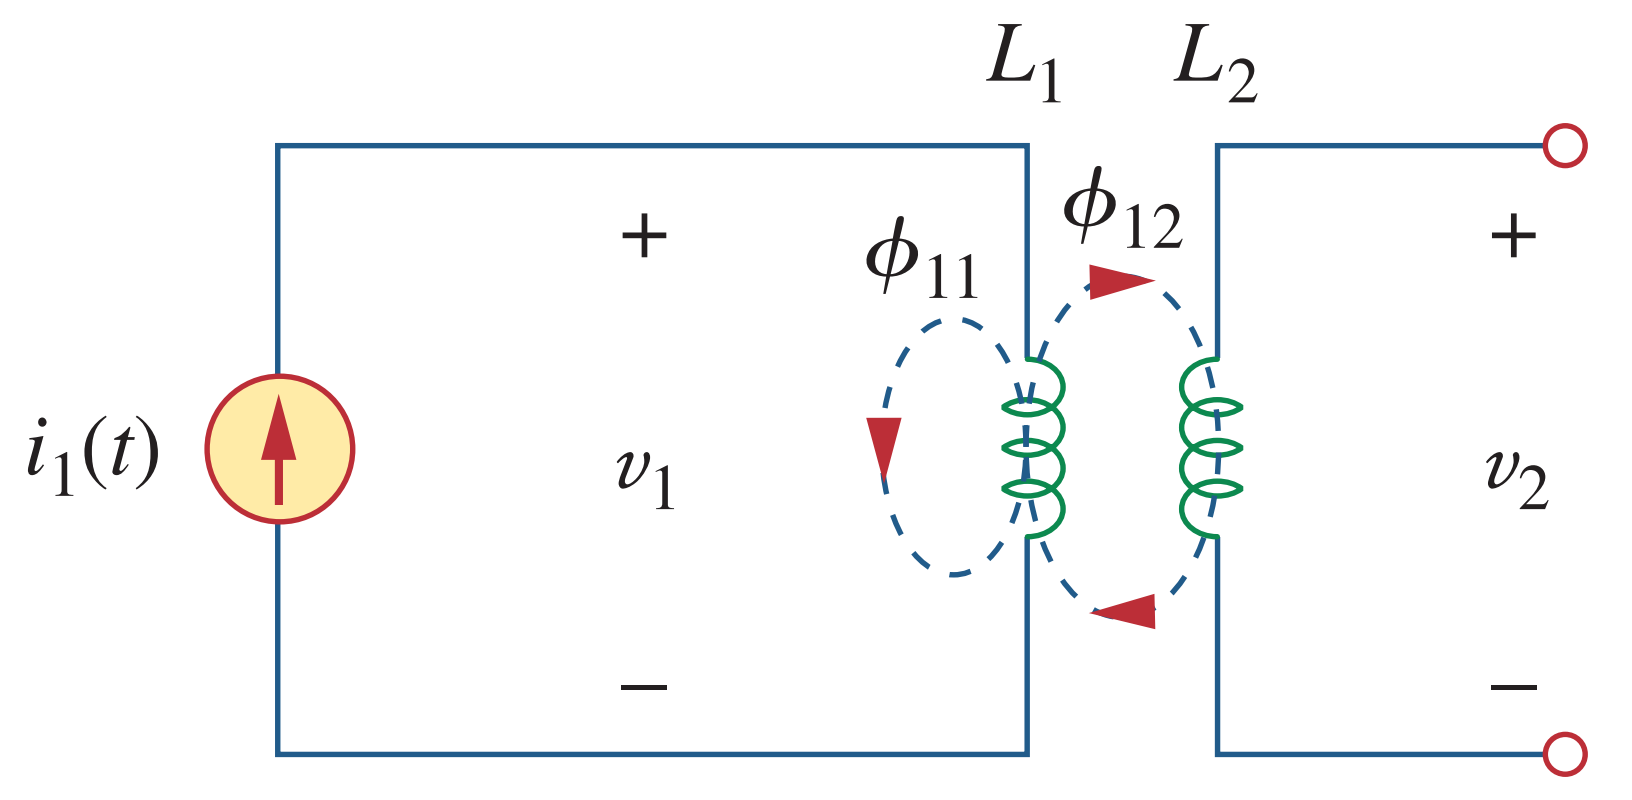
\includegraphics[width=0.55\textwidth]{C13/intro.png}
\end{figure}


In this case, additional inductance will be generated on both coils, which is called the \textbf{mutual inductance} $M$, with the same unit $\mathrm{H}$ as self-inductance $L$.

\begin{small}
    (You don't need to be familiar with the derivation (textbook p557-558).)   
\end{small}

\end{frame}

%%%%%%%%%%%%%%%%%%%%%%%%%

\begin{frame}{Mutual Voltage}
    
The existence of mutual inductance will induce voltage in both coils, called \textbf{mutual voltage}. This induced voltage must be taken into consideration if we want to analyze the circuit as before. 

\begin{figure}[H]
    \centering
    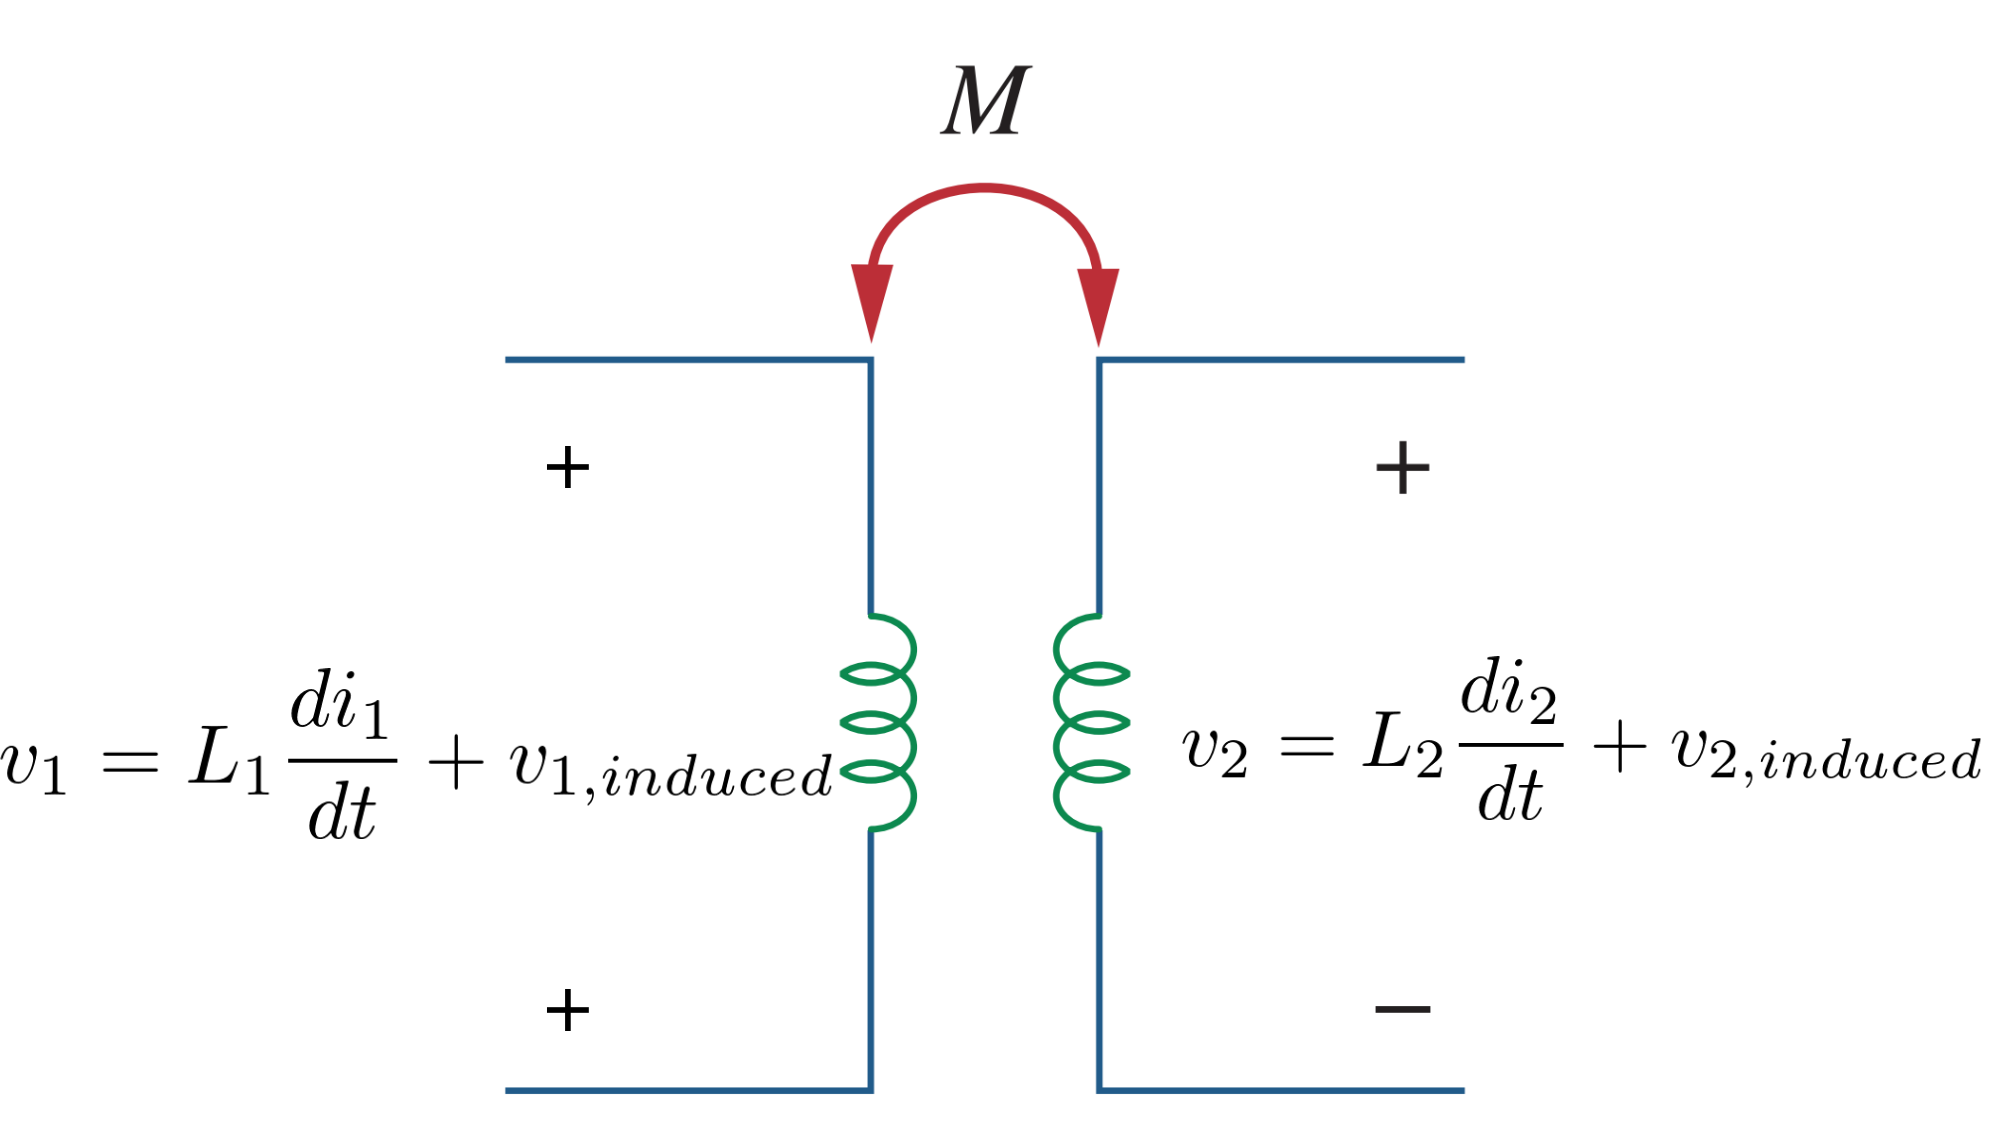
\includegraphics[width=0.75\textwidth]{C13/ill.png}
\end{figure}



\end{frame}

%%%%%%%%%%%%%%%%%%%%%%%%%

\begin{frame}{Mutual Voltage}

The magnitude of the mutual voltage on each side are
$$
    \begin{aligned}
        \vert v_{\color{red}1\color{black},induced} \vert &= \vert M\frac{di_{\color{red}2\color{black}}}{dt}\vert\\
        \vert v_{\color{red}2\color{black},induced} \vert &= \vert M\frac{di_{\color{red}1\color{black}}}{dt} \vert
    \end{aligned}
$$
The form of the formula is the same as the i-v relationship of an inductor, but be careful that the induced voltage on one coil is jointly determined by both $M$ and \color{red} the current in the other coil\color{black}.

\end{frame}

%%%%%%%%%%%%%%%%%%%%%%%%%
\begin{frame}{Mutual Voltage: Dot Convention}

The direction is determined by the \textbf{dot convention}.
%which exempts us from dealing with the concrete structure of the coils.

\vspace{0.3cm}

\begin{itemize}
    \item If a current \color{red}enters \color{black} the dotted terminal of one coil, the reference polarity of the mutual voltage in the second coil is positive at the dotted terminal of the second coil.
    \item If a current leaves the dotted terminal of one coil, the reference polarity of the mutual voltage in the second coil is negative at the dotted terminal of the second coil.
\end{itemize}


% The mutual voltage depends on how to set directions of current $I_1$ and $I_2$.
% \begin{figure}[H]
%         \centering
%         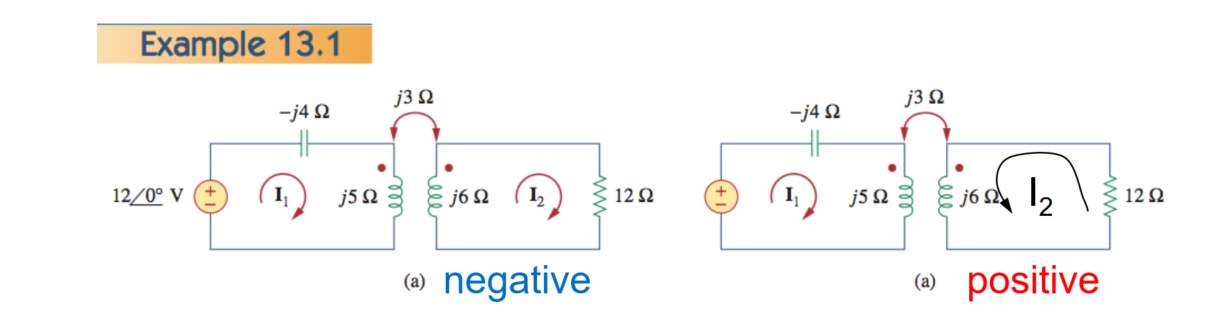
\includegraphics[width=1\textwidth]{C13/2.png}
%     \end{figure}
\end{frame}

%%%%%%%%%%%%%%%%%%%%%%%%%
\begin{frame}{Mutual Voltage: Dot Convention}

\begin{table}[]
    \centering
    \begin{tabular}{c|c}

        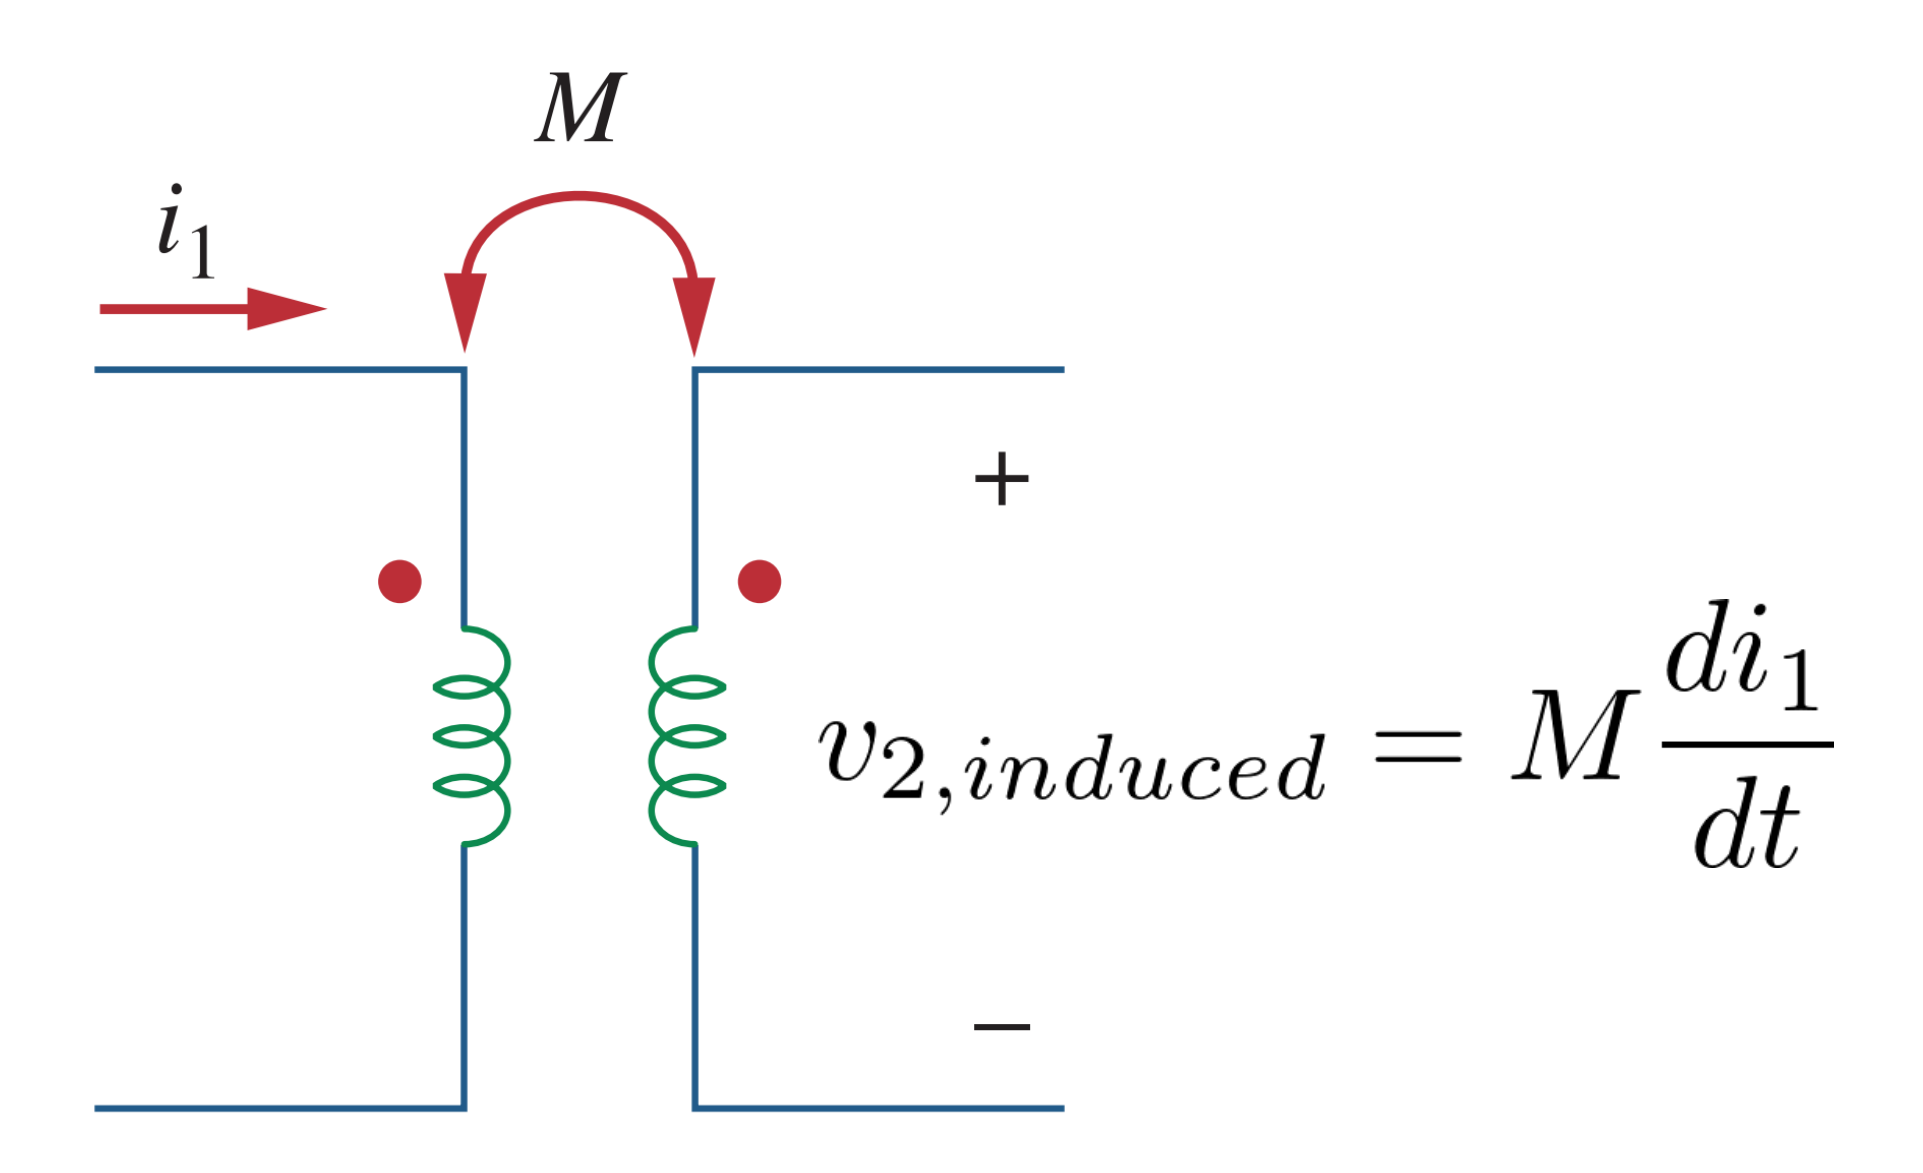
\includegraphics[width=0.42\textwidth]{C13/case11.png}
         &
        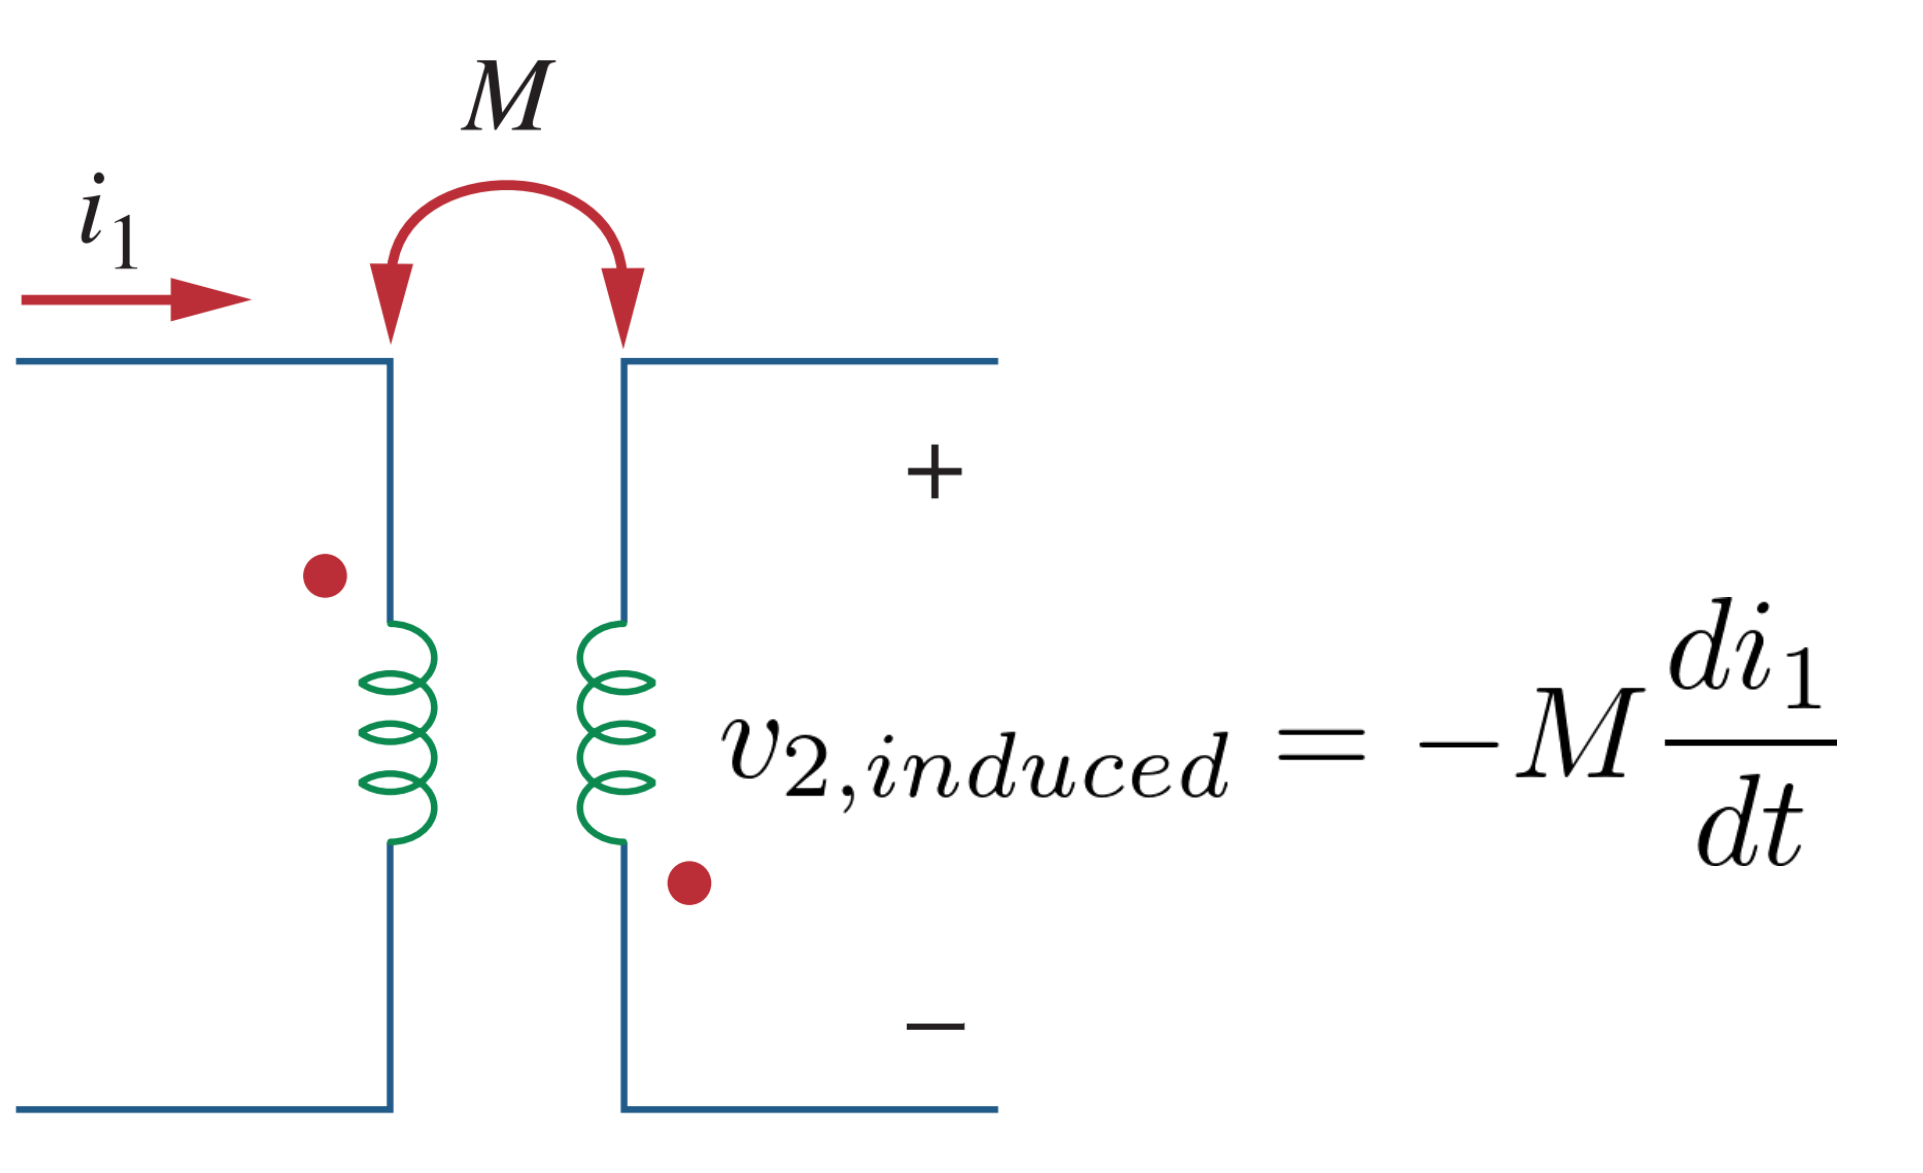
\includegraphics[width=0.42\textwidth]{C13/case22.png}
         \\
         Case 1 & Case 1 \\
        \hline
        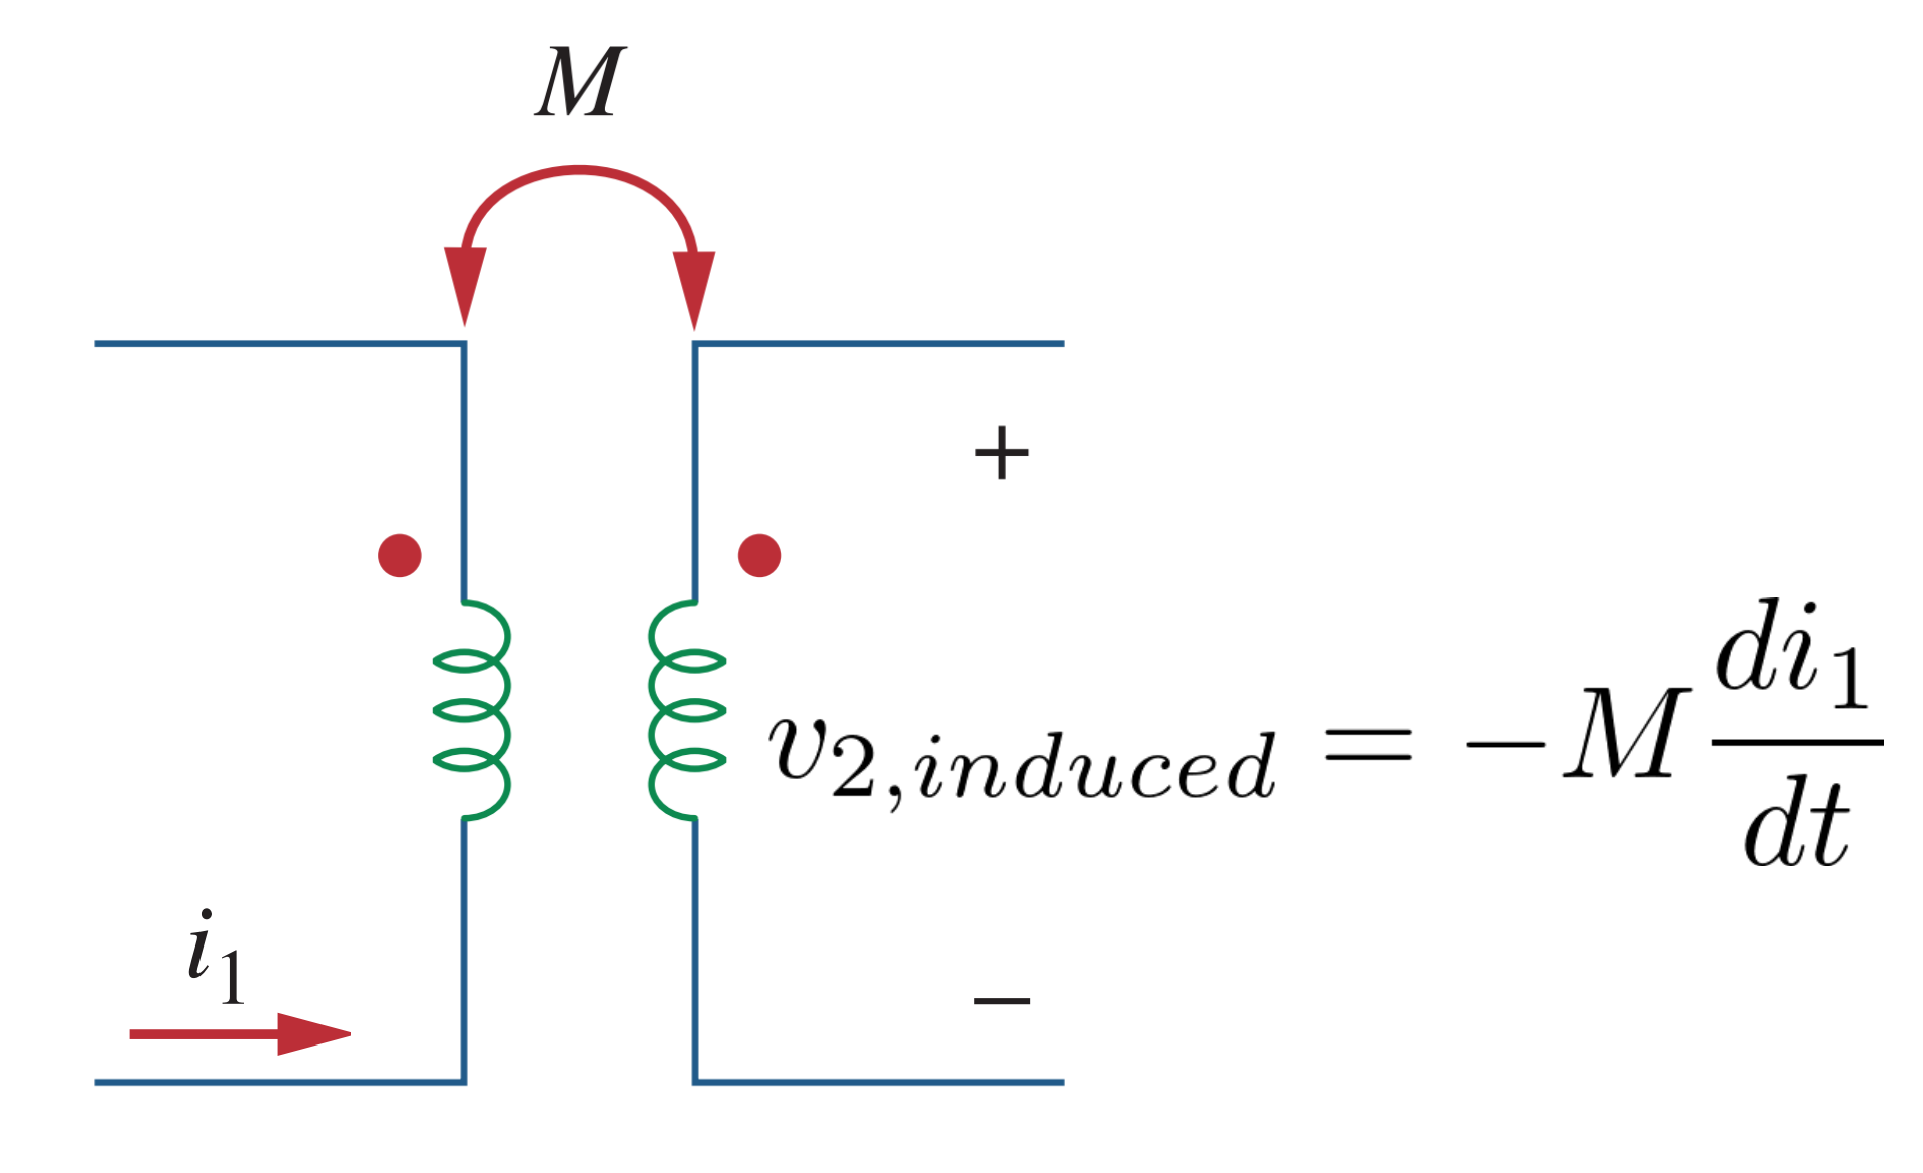
\includegraphics[width=0.42\textwidth]{C13/case33.png}
         &
        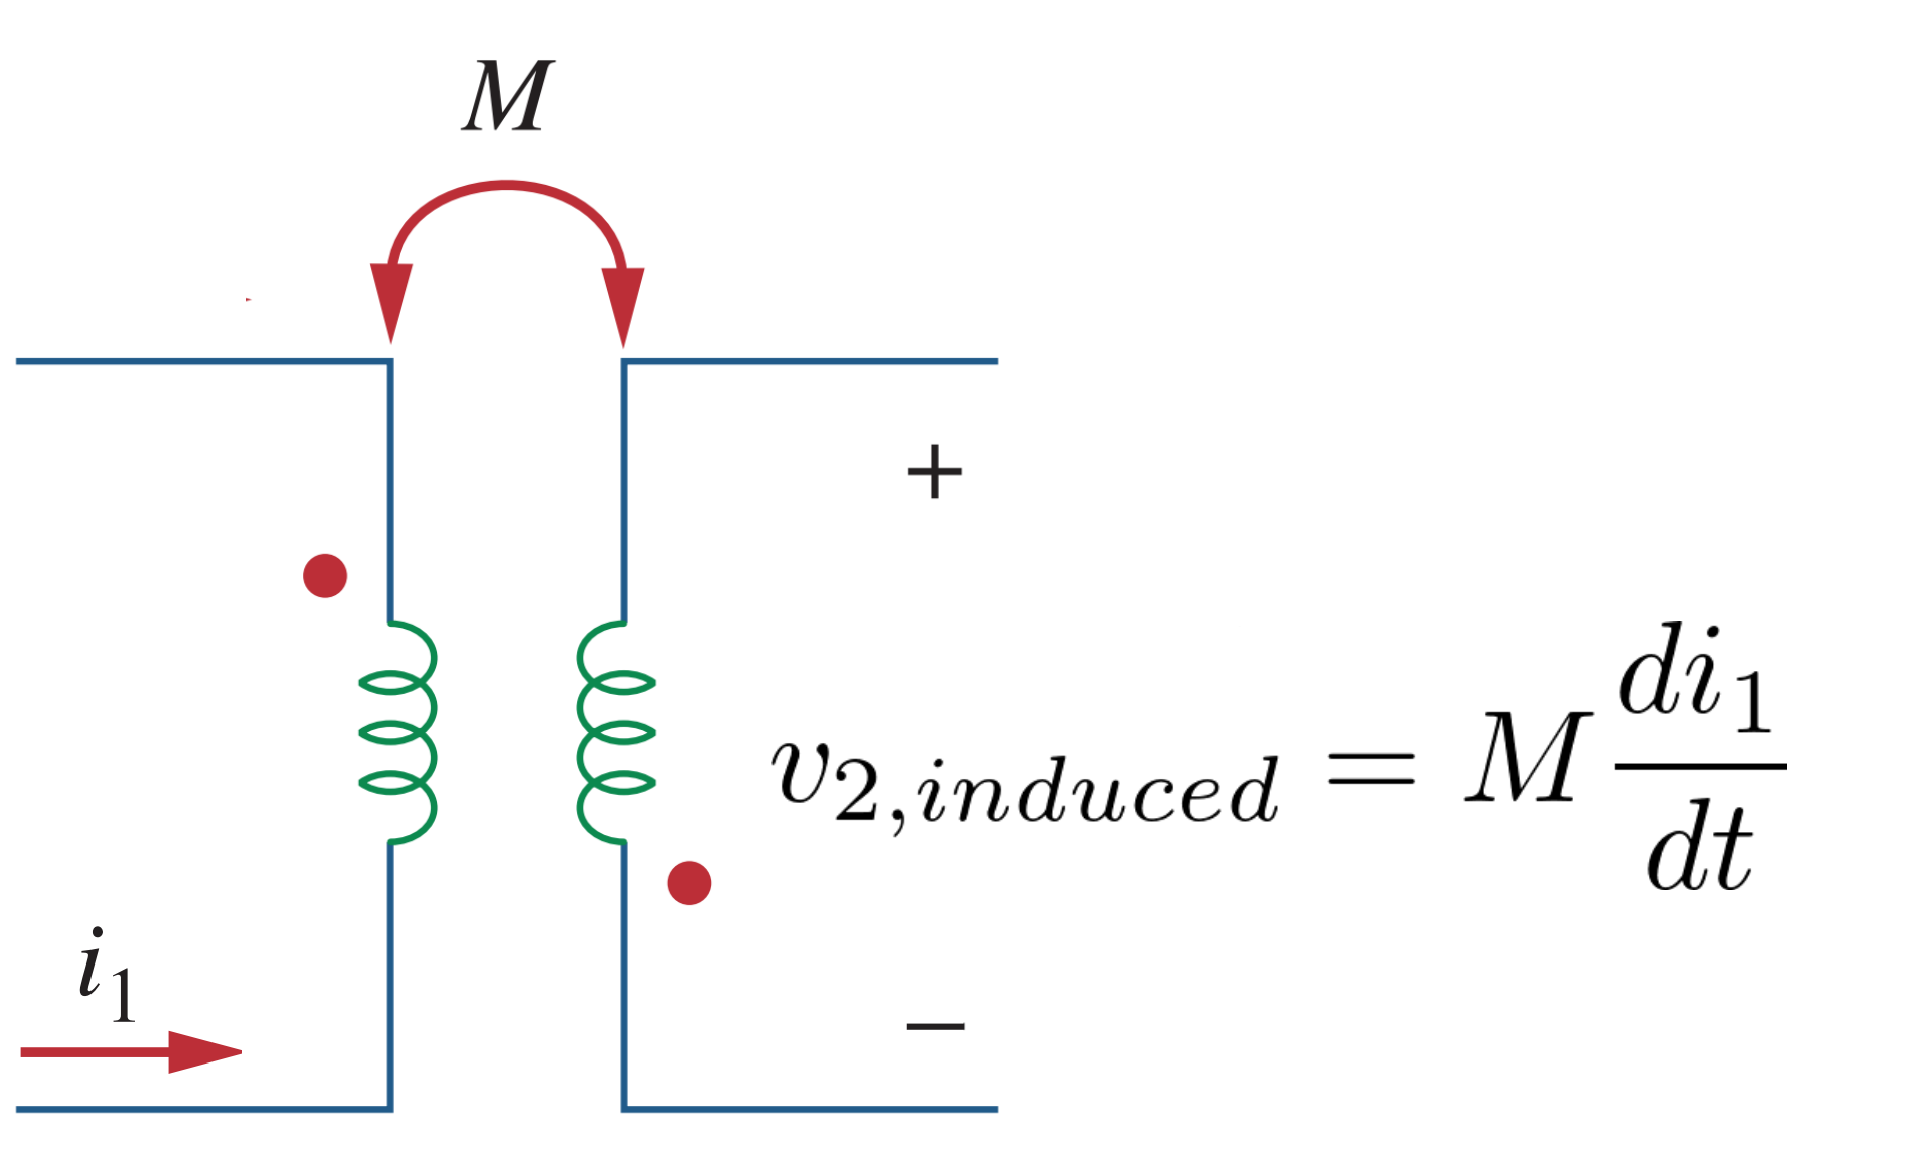
\includegraphics[width=0.42\textwidth]{C13/case44.png}
         \\
         Case 2 & Case 2 \\
    \end{tabular}

\end{table}
\end{frame}


%%%%%%%%%%%%%%%%%%%%%%%%%

\begin{frame}{Applying KCL}
KCL for magnetically coupled circuit is basically the same as before. Only to pay attention to the dot convention.\\
In the following circuit, $I_1$ enters the node, $I_2$ leaves the node. So mutual voltage is negative.
\begin{figure}[H]
        \centering
        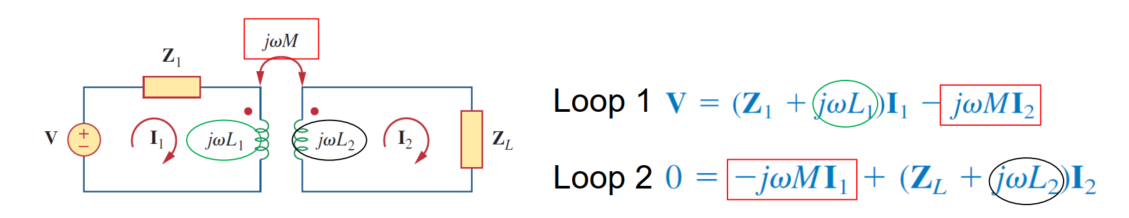
\includegraphics[width=1\textwidth]{C13/3.png}
    \end{figure}
\end{frame} 

%%%%%%%%%%%%%%%%%%%%%%%%%
\begin{frame}{Apply KCL: Physically Not Connected}
To make the analysis easier, we assign a dependent voltage based on the sign of the mutual voltage.
\begin{figure}[H]
        \centering
        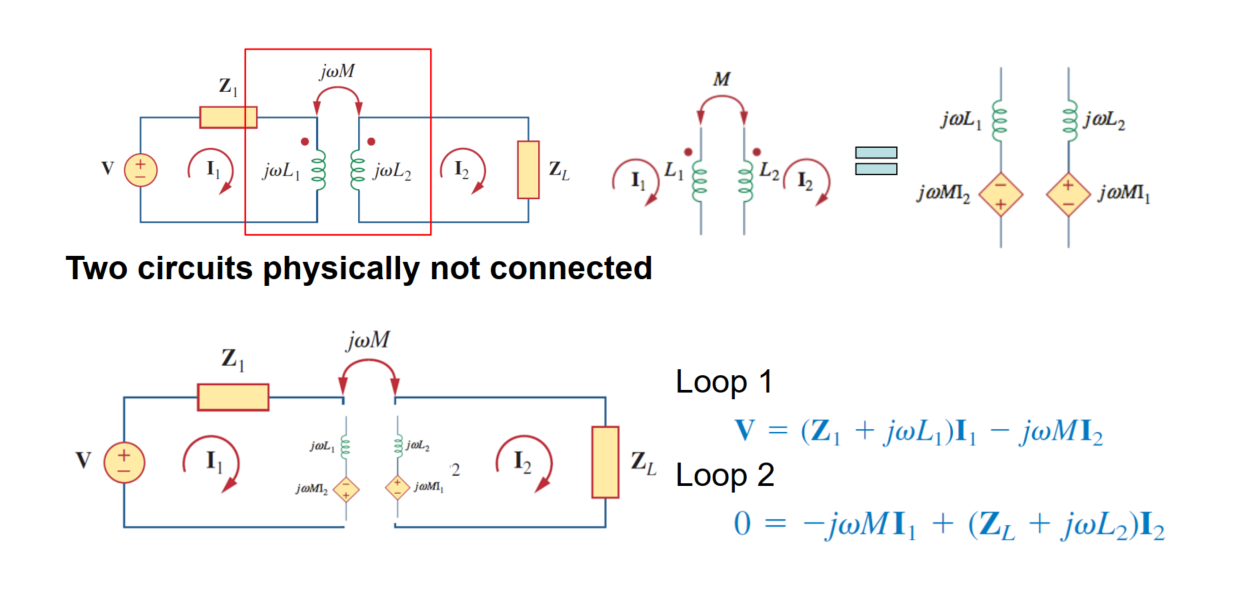
\includegraphics[width=1\textwidth]{C13/4.png}
    \end{figure}
\end{frame}

%%%%%%%%%%%%%%%%%%%%%%%%%

\begin{frame}{Apply KCL: Physically Connected} % Need to use the fragile option when verbatim is used in the slide
For circuit physically connected, pay attention to the values and polarity.
\begin{figure}[H]
        \centering
        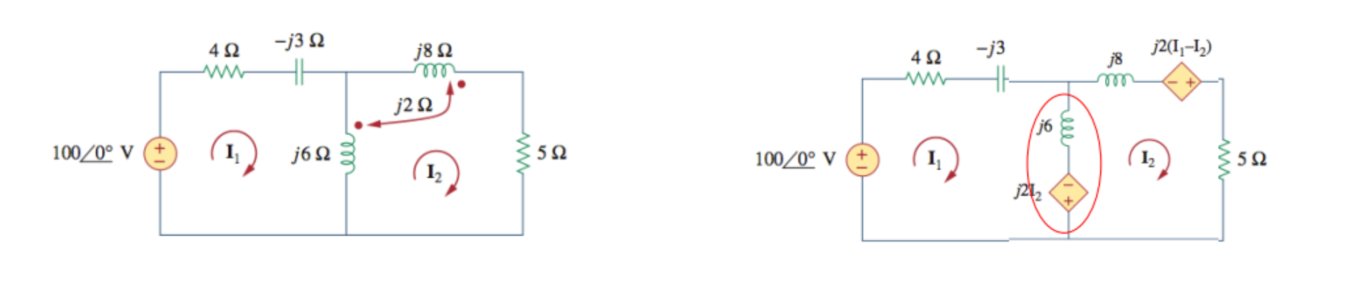
\includegraphics[width=1\textwidth]{C13/5.png}
    \end{figure}
    \begin{figure}[H]
        \centering
        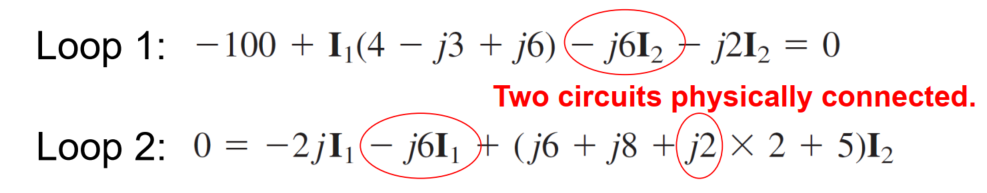
\includegraphics[width=1\textwidth]{C13/6.png}
    \end{figure}
\end{frame}

%%%%%%%%%%%%%%%%%%%%%%%%%

\begin{frame}{Exercise}

Obtain the Norton equivalent at terminals $a-b$ of the circuit in the following circuit.

\begin{figure}[H]
        \centering
        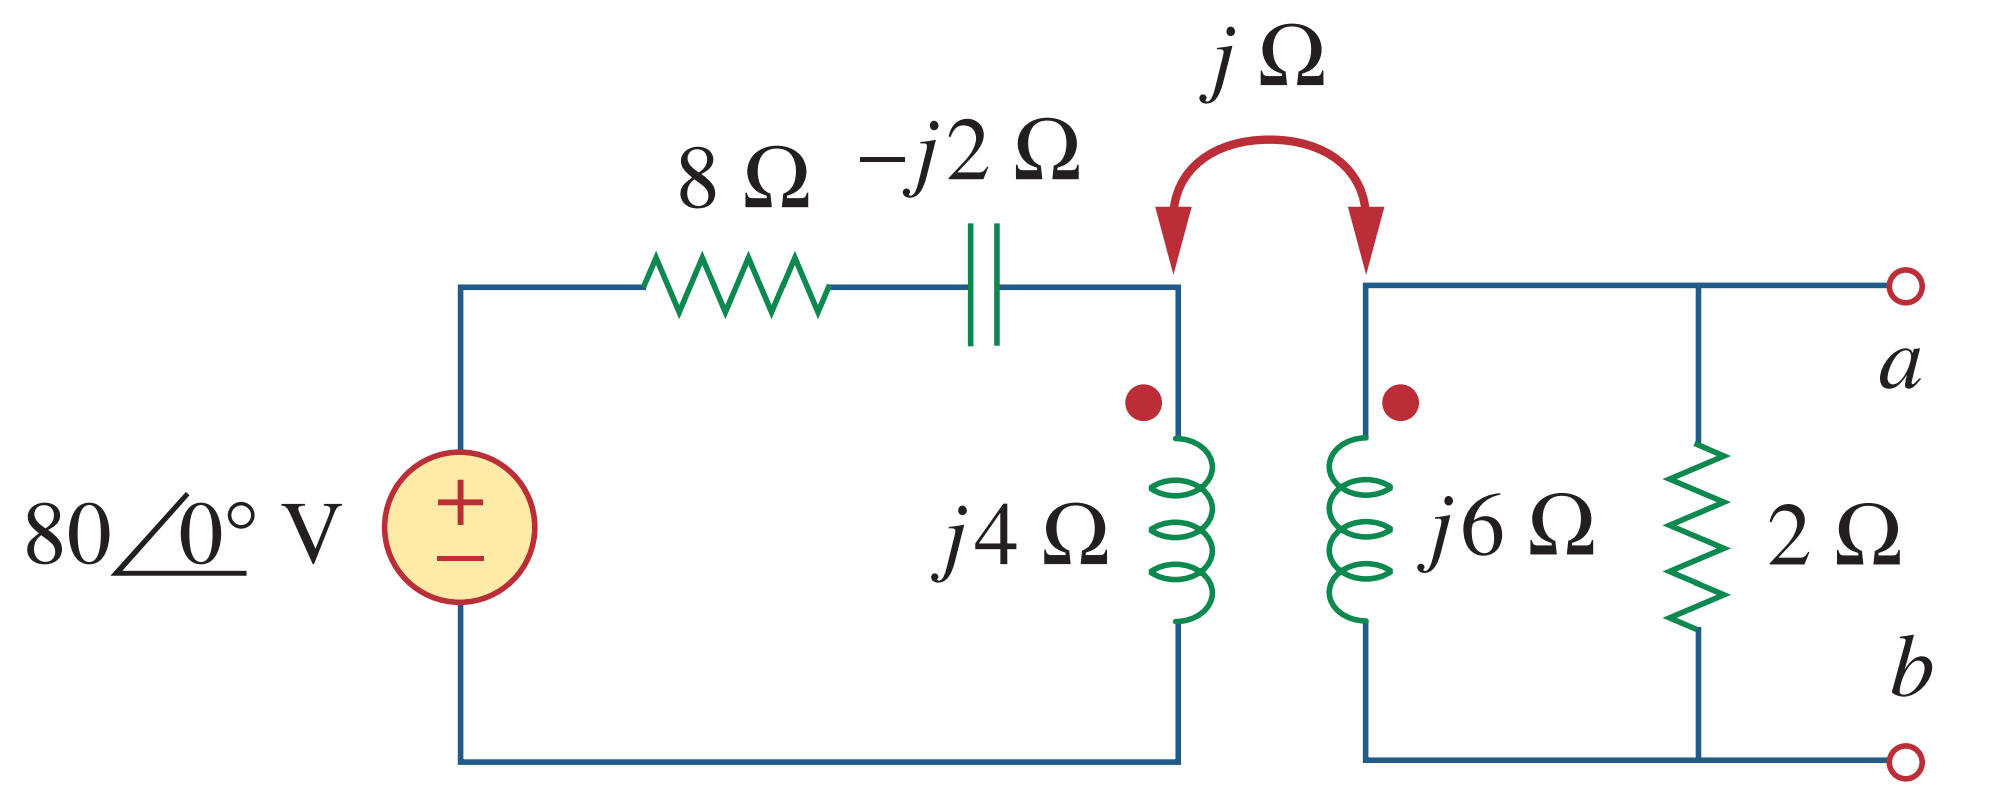
\includegraphics[width=0.7\textwidth]{C13/11.png}
    \end{figure}
\end{frame}

%%%%%%%%%%%%%%%%%%%%%%%%%

\begin{frame}{Energy in a Coupled Circuit}

The energy stored in a coupled circuit is

$$w = \frac12L_1i_1^2(t)+\frac12L_2i_2^2(t) \color{red}\pm\color{black} i_1(t)i_2(t)$$

Minus sign occurs when the mutual voltage is negative, i.e., current enters one dotted terminal and leaves the other dotted terminal.

\begin{small}
   ($i_1(t)$, $i_2(t)$ should be sinusoidal. Plug in value of $t$ in calculation.)
\end{small}


\vspace{0.3cm}
\noalign \hline
\vspace{0.3cm}

The coupling coefficient 
$$k = \frac{M}{L_1L_2}$$
describes the extent to which $M$ approaches $\sqrt{L_1L_2}$.

$k > 0.5 \rightarrow$ loosely coupled, $k > 0.5 \rightarrow$ tightly coupled.


\end{frame}

%%%%%%%%%%%%%%%%%%%%%%%%%

% \begin{frame}{Exercise}


% \begin{figure}[H]
%         \centering
%         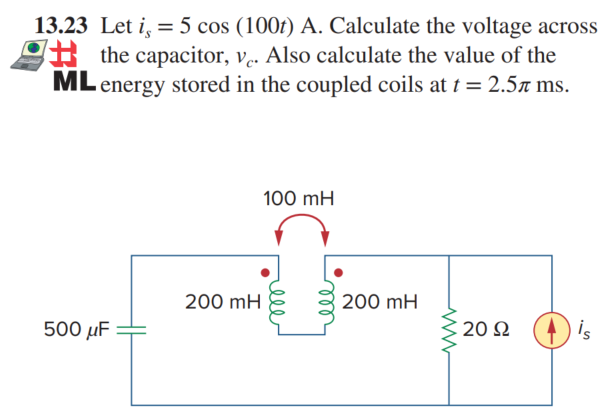
\includegraphics[width=0.6\textwidth]{C13/14.png}
%     \end{figure}
% \end{frame}

%%%%%%%%%%%%%%%%%%%%%%%%%

\begin{frame}{Transformers}

A transformer is a four-terminal circuit element comprising two magnetically coupled coils.

\begin{figure}[H]
    \centering
    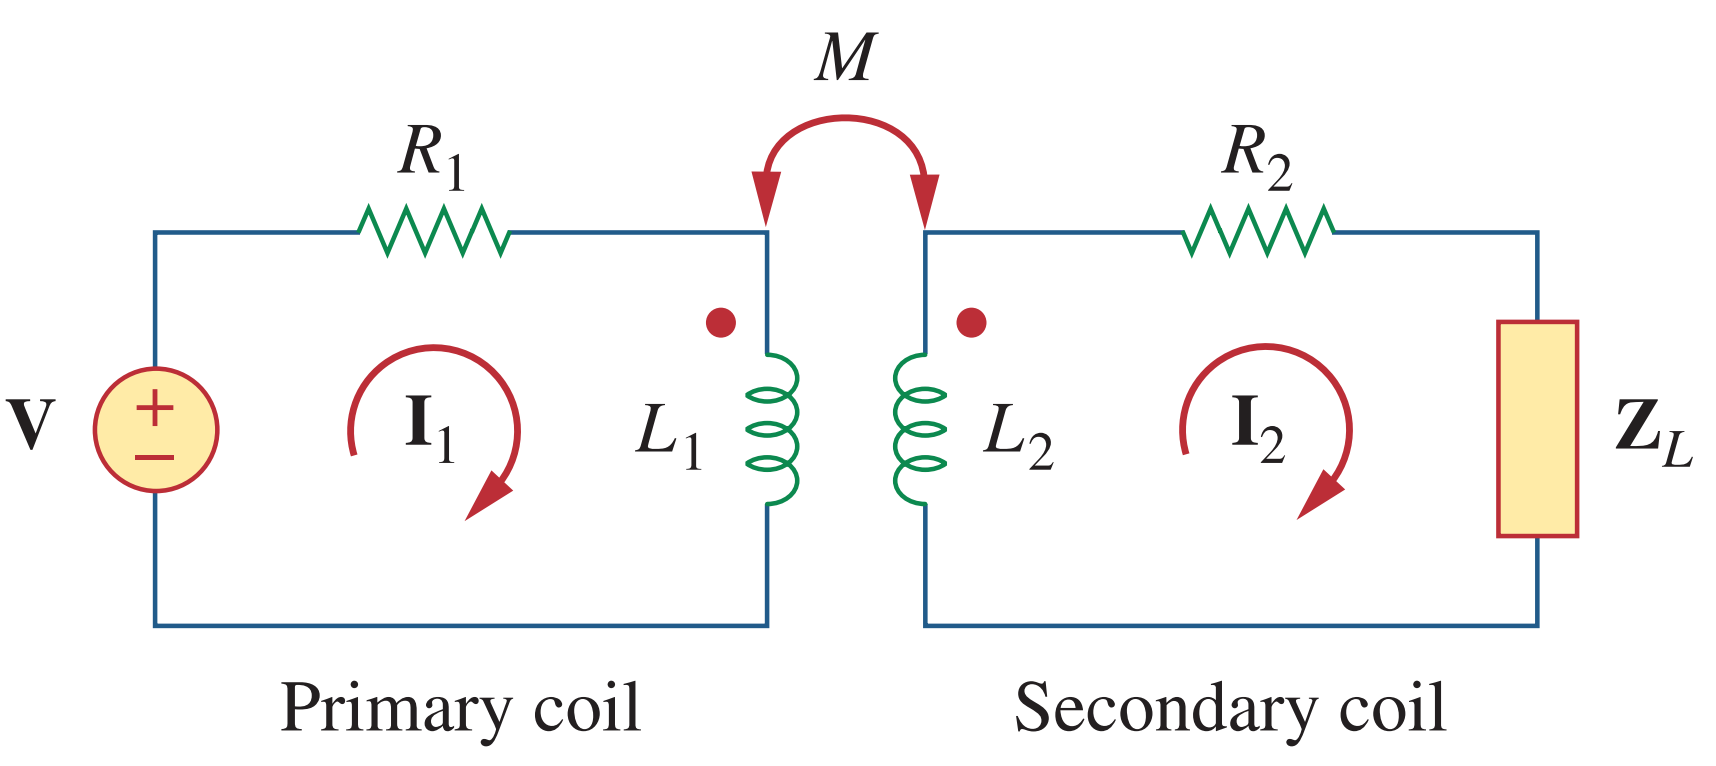
\includegraphics[width=0.55\textwidth]{C13/lin tra.png}
\end{figure}


% \vspace{0.3cm}
% \noalign \hline
% \vspace{0.3cm}

% The input impedance $Z_{in}$:
% $$Z_{in} = \frac{\tilde{V}}{\tilde{I}} = R_1+j\omega L + \frac{\omega^2M^2}{R_2+j\omega L_2+Z_L}$$

\end{frame}

%%%%%%%%%%%%%%%%%%%%%%%%%

\begin{frame}{Transformers}
It is convenient to replace a transformer by an equivalent circuit with no magnetic coupling.

\begin{itemize}
    \item When two dots are on the same side:
    \begin{table}[]
    \centering
    \begin{tabular}{cc}
        \toprule
         Equivalent T circuit & Equivalent $\Pi$ circuit  \\
         \midrule
         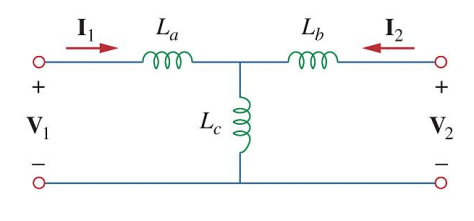
\includegraphics[width=0.4\textwidth]{C13/16.png}
         &
         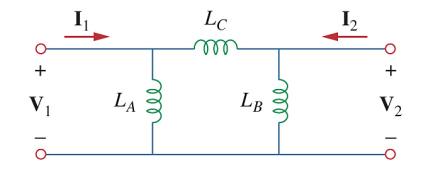
\includegraphics[width=0.4\textwidth]{C13/17.png}
         \\
         $L_a = L_1-M$ 
         &
         $L_A = \frac{L_1L_2 - M^2}{L_2-M}$
         \\
          $L_b = L_2 - M$
          &
          $L_B = \frac{L_1L_2 - M^2}{L_1-M}$
          \\
            $L_c = M$
          &
            $L_C = \frac{L_1L_2 - M^2}{M}$
          \\
         \bottomrule
    \end{tabular}

    \end{table}
    
    \item When two dots are on opposite sides, \color{red} replace all $M$ by $-M$\color{black}.
\end{itemize}

\end{frame}


%%%%%%%%%%%%%%%%%%%%%%%%%
\begin{frame}{Ideal Transformers}

An \textbf{ideal transformer} is one with perfect coupling ($k=1$). With this idealization, we have a quite simple relationship for the currents and voltages at both sides:
$$\vert \frac{\tilde{V_2}}{\tilde{V_1}} \vert = \vert \frac{\tilde{I_1}}{\tilde{I_2}} \vert = \frac{N_2}{N_1} = n $$

The rules for determining the sign:
\begin{itemize}
    \item For $\tilde{V}$: If $\tilde{V_1}$ and $\tilde{V_2}$ are both positive or both negative at the dotted terminal, $\tilde{V_2} / \tilde{V_1} = \color{red}+n\color{black}$, otherwise  $\tilde{V_2} / \tilde{V_1} = \color{red}-n\color{black}$.
    \item for $\tilde{I}$: If $\tilde{I_1}$ and $\tilde{I_2}$ both enter or both leave the dotted terminals, $\tilde{I_1}/\tilde{I_2} = \color{red}-n\color{black}$, otherwise $\tilde{I_1}/\tilde{I_2} = \color{red}+n\color{black}$,
\end{itemize}
% V2 / V1 = I1 / I2 = \pm N2 / N1 = \pm n


\end{frame}

%%%%%%%%%%%%%%%%%%%%%%%%%

\begin{frame}{Ideal Transformers}

\begin{table}[]
    \centering
    \begin{tabular}{c|c}
        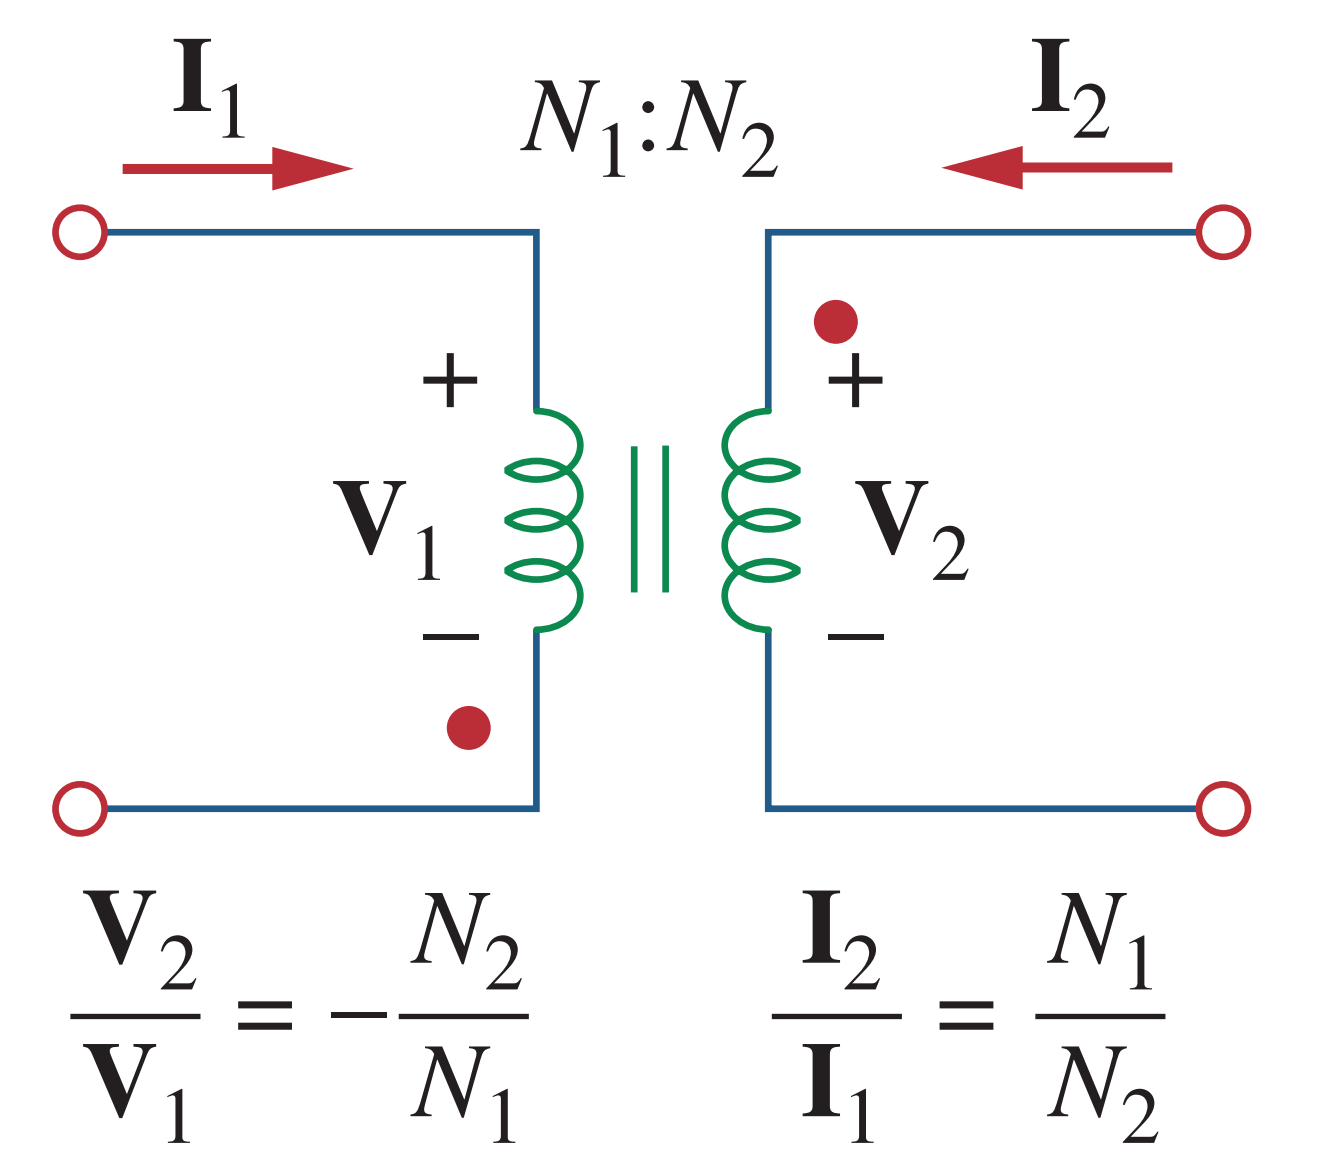
\includegraphics[width=0.35\textwidth]{C13/case811.png}
         &
        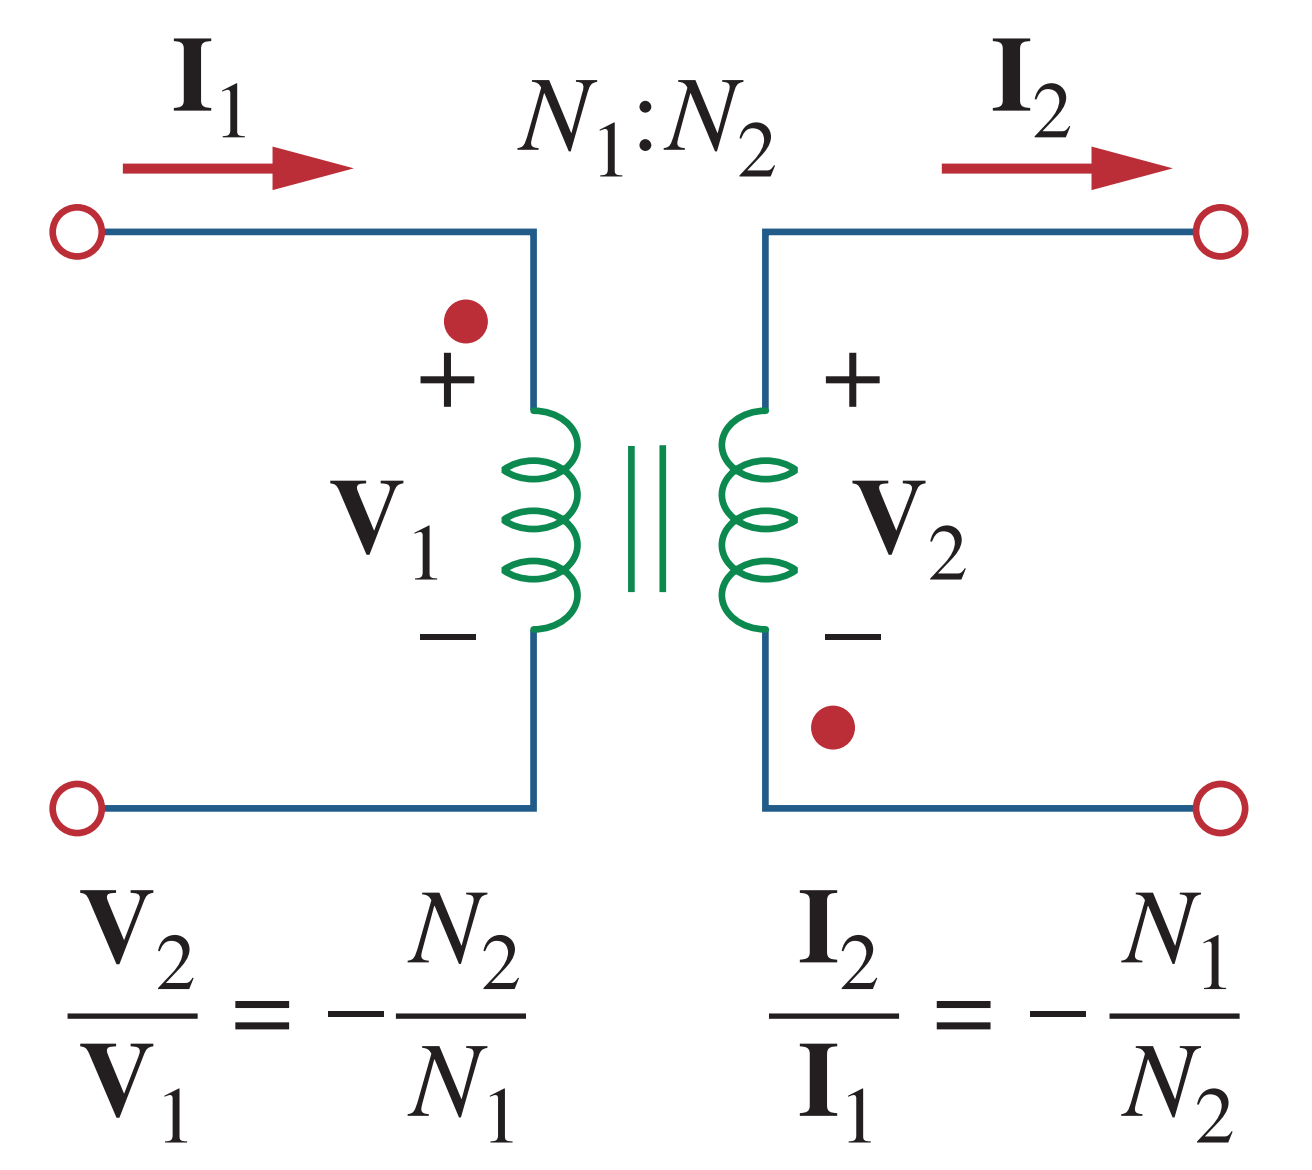
\includegraphics[width=0.35\textwidth]{C13/case822.png}
         \\
         % Case 1 & Case 1 \\
        \hline
        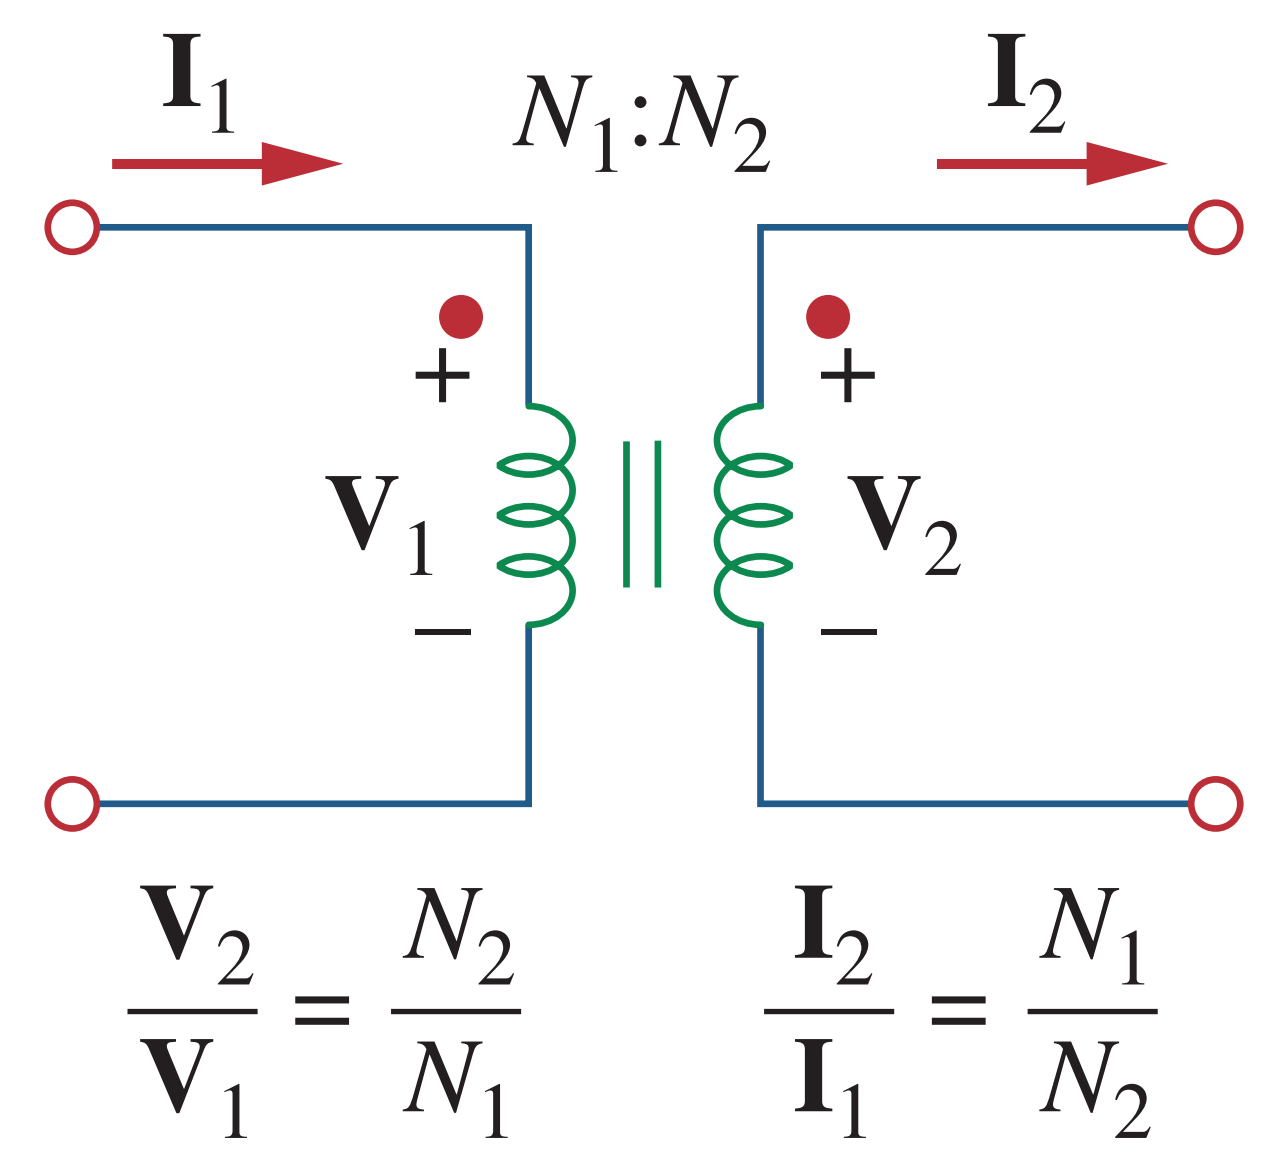
\includegraphics[width=0.35\textwidth]{C13/case833.png}
         &
        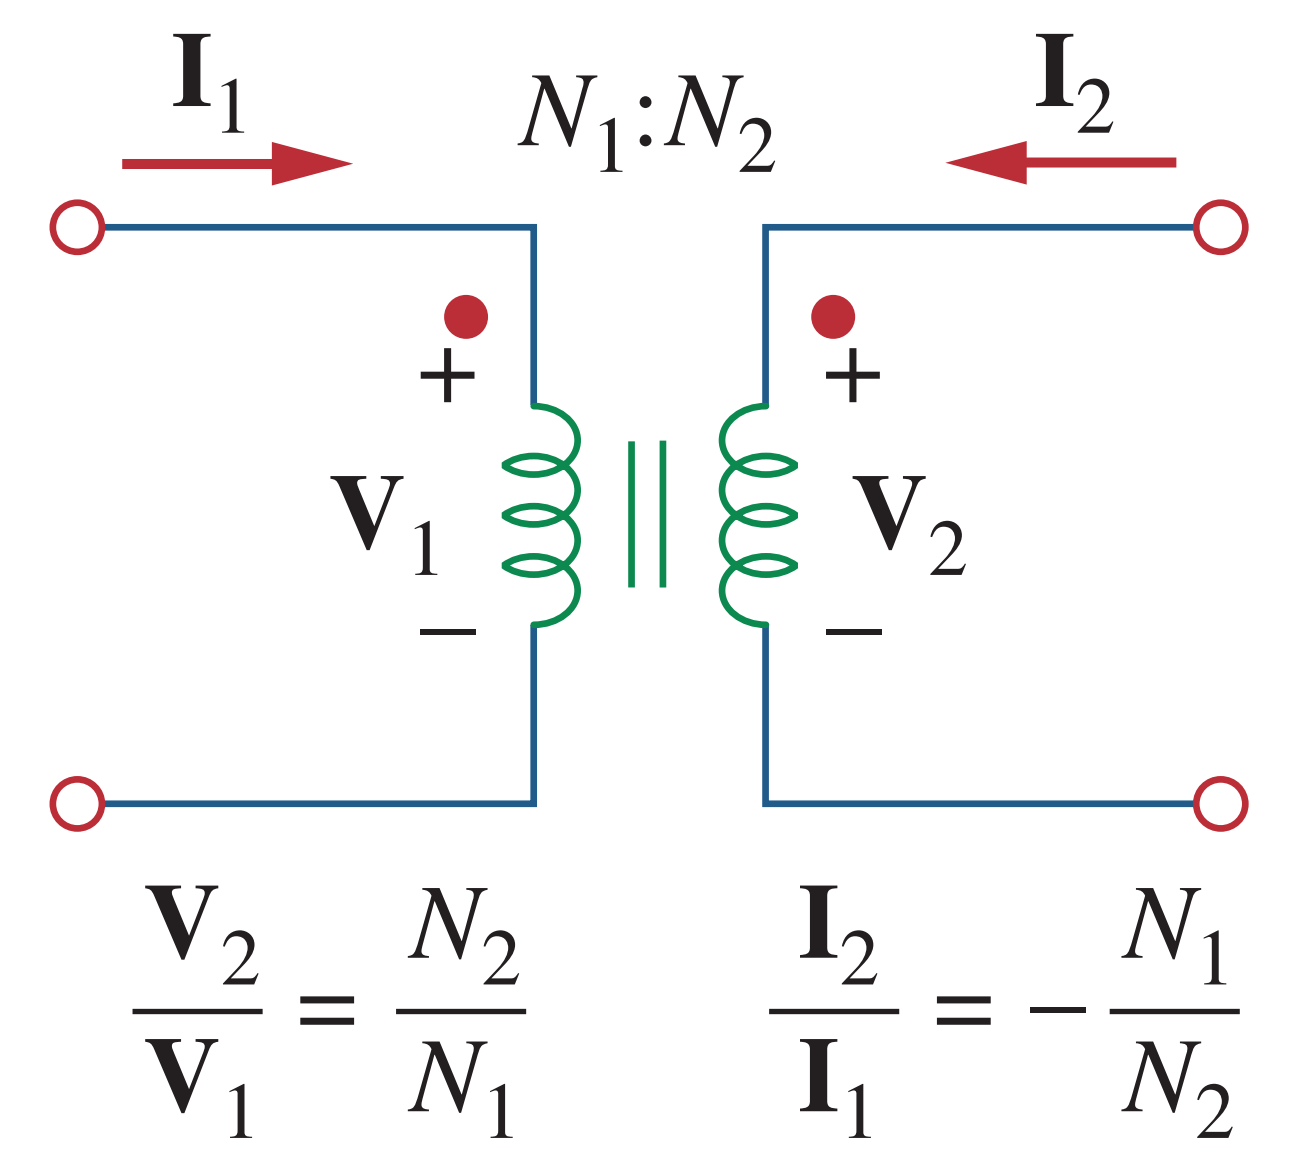
\includegraphics[width=0.35\textwidth]{C13/case844.png}
         \\
         % Case 2 & Case 2 \\
    \end{tabular}

\end{table}

\end{frame}
%%%%%%%%%%%%%%%%%%%%%%%%%

\begin{frame}{Ideal Transformers: Equivalent Circuit}
It is more convenient to replace the transformer with an equivalent circuit.

\begin{figure}[H]
        \centering
        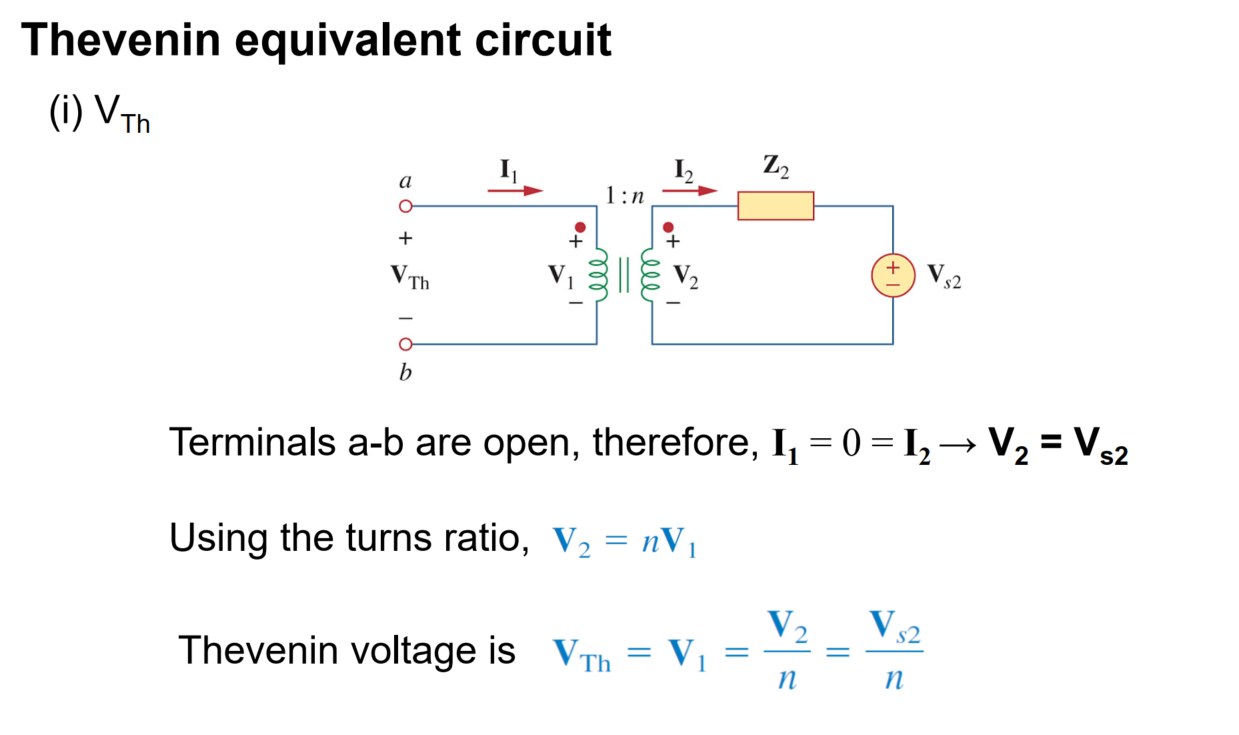
\includegraphics[width=0.9\textwidth]{C13/9.png}
    \end{figure}
\end{frame}

\begin{frame}{Ideal Transformers: Equivalent Circuit}
It is more convenient to replace the transformer with a normal circuit.

\begin{figure}[H]
        \centering
        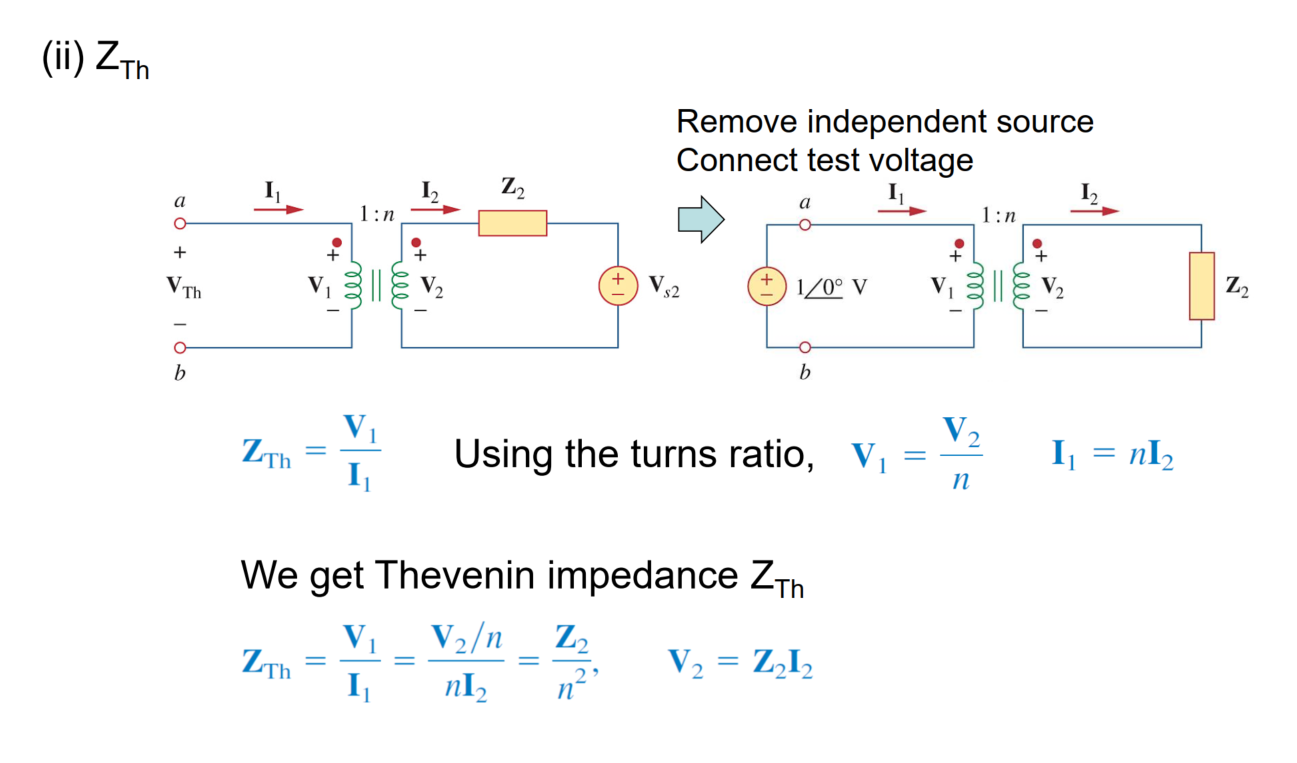
\includegraphics[width=0.9\textwidth]{C13/10.png}
    \end{figure}
\end{frame}

\begin{frame}{Ideal Transformers: Equivalent Circuit}
Overall, 
$$\mathbf{V}_{th}=\frac{\mathbf{V}_{s2}}{n} \qquad \mathrm{Z}_{th} = \frac{\mathbf{Z}_2}{n^2}$$

\begin{figure}[H]
        \centering
        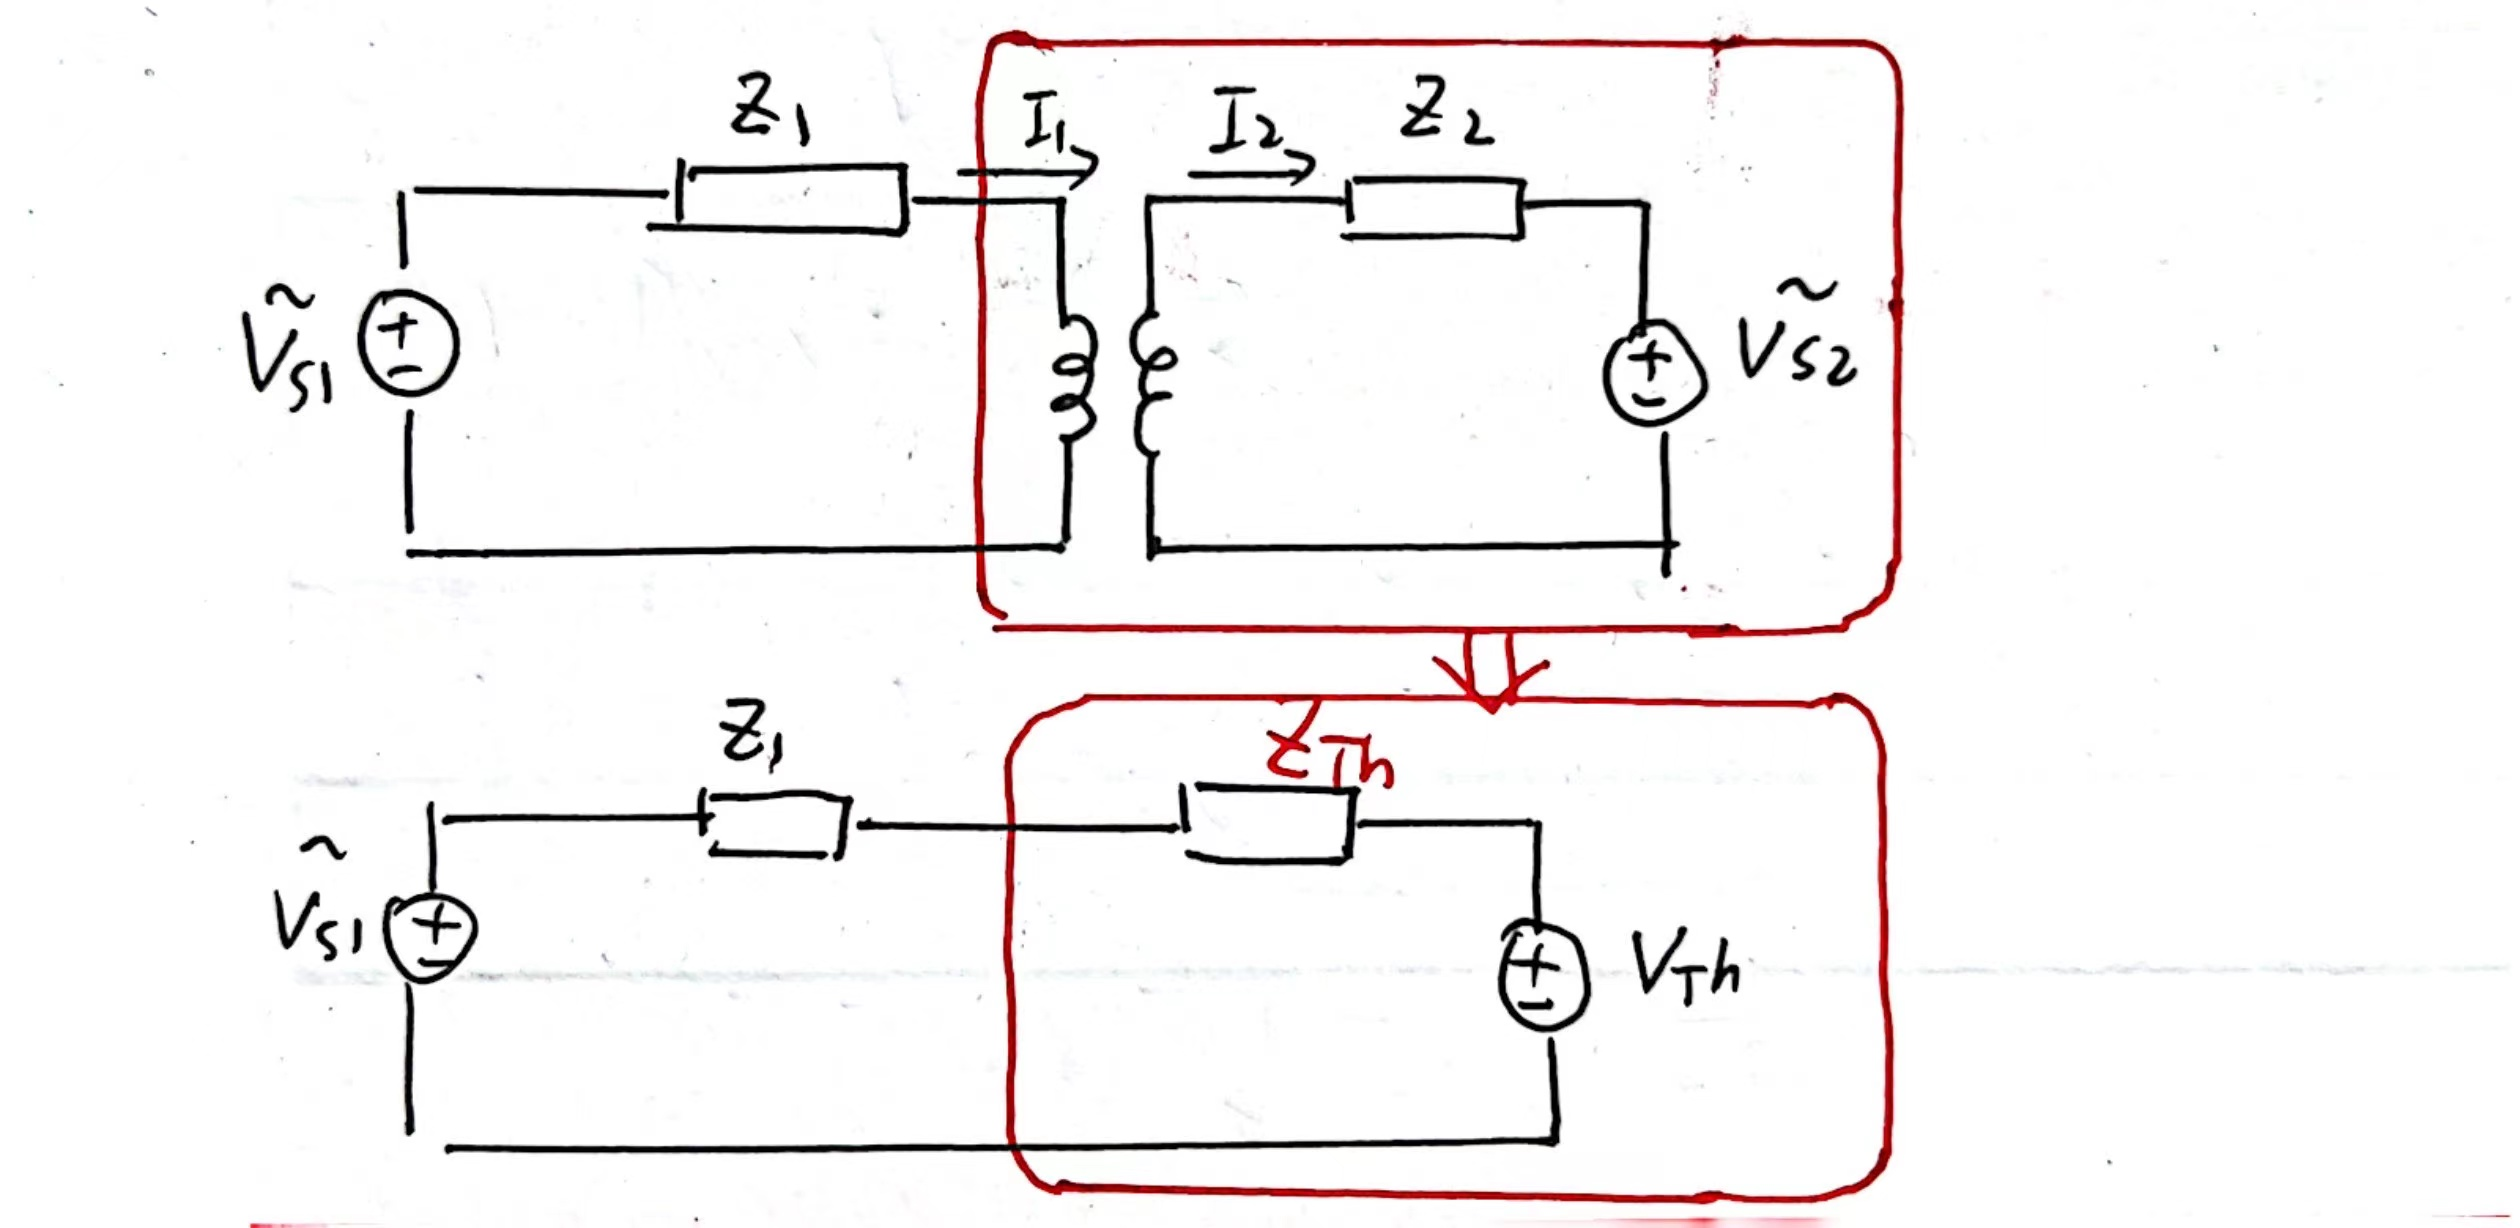
\includegraphics[width=0.9\textwidth]{C13/equi.jpeg}
\end{figure}
\end{frame}

%%%%%%%%%%%%%%%%%%%%%%%%%
\begin{frame}{Exercise}

Find $v(t)$ in the following circuit.
\begin{figure}[H]
        \centering
        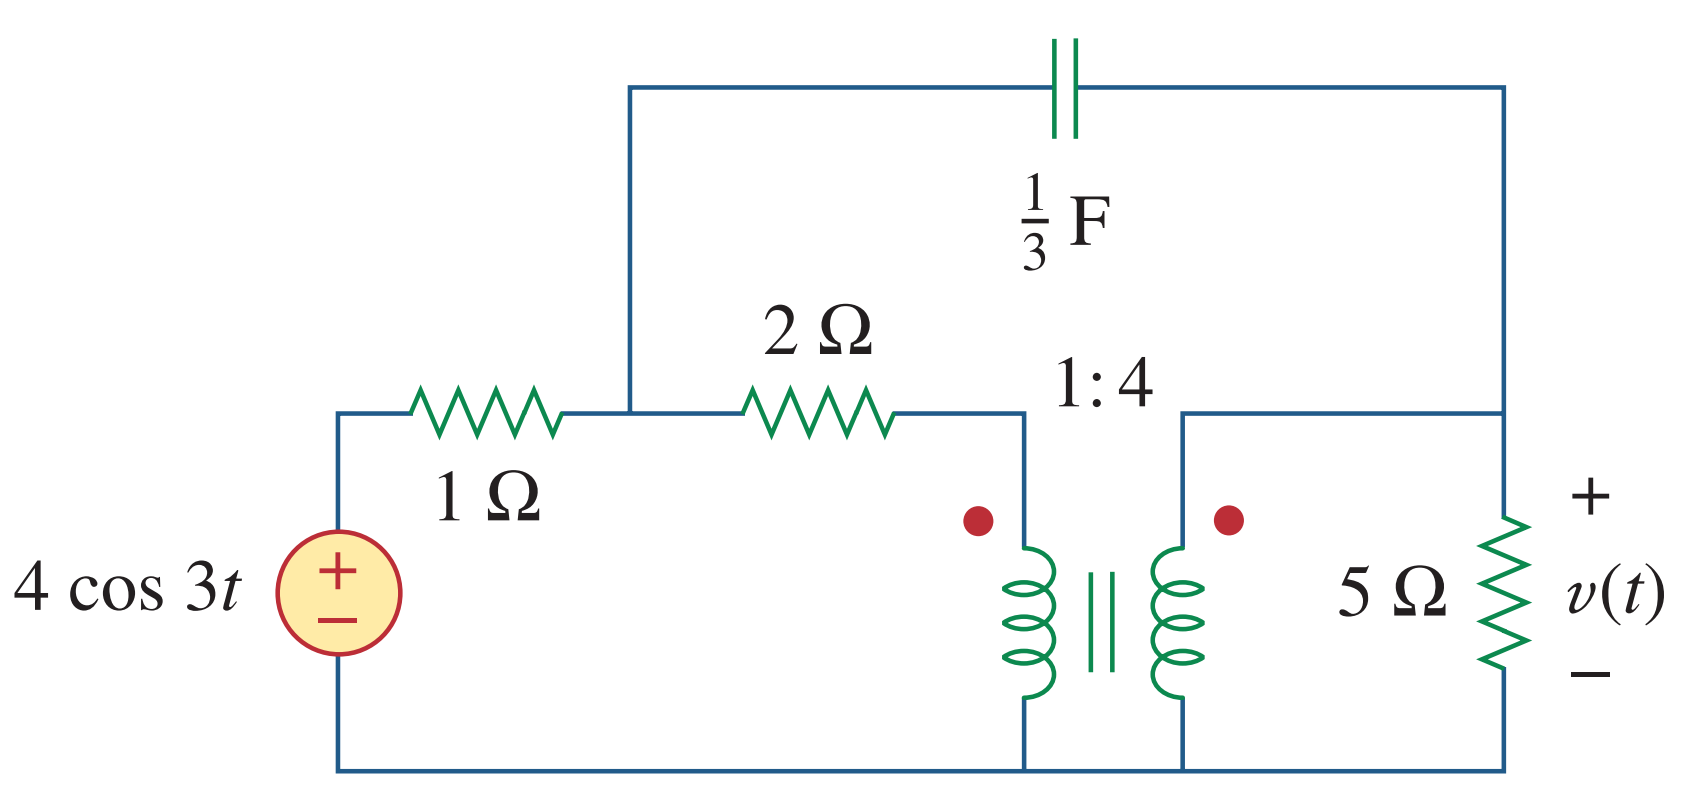
\includegraphics[width=0.7\textwidth]{C13/12.png}
    \end{figure}
\end{frame}


%%%%%%%%%%%%%%%%%%%%%%%%%%%%%%%%%%%%%%%%%%%%%%%
% FREQUENCY RESPONSE

\section{Frequency Response}

%%%%%%%%%%%%%%%%%%%%%%%%%
\begin{frame}{Frequency Response}

Motivation: previously we analyzed all the AC circuits with frequency $\omega$ fixed. Now we study how a circuit's behavior varies with change in frequency. This variation is so-called the \textbf{frequency response}.

\vspace{0.3cm}

Specifically, we want to study the ratio of two phasor signals, as a function of frequency $\omega$, i.e. the \textbf{transfer function}

$$\mathbf{H}(\omega) = \frac{\mathbf{Y}(\omega)}{\mathbf{X}(\omega)}$$


\end{frame}

%%%%%%%%%%%%%%%%%%%%%%%%%

\begin{frame}{Transfer Function}

The transfer function $\mathbf{H}(\omega)$ can always be expressed in the ratio of two polynomials. Also, \color{red} actually every $\omega$ in the function takes with a $j$ \color{black} (no need to worry about why in VE215). So often we let the variable be $j\omega$ instead of $\omega$, let $s = j\omega$, we have

$$\mathbf{H}(\omega) = \mathbf{H}(j\omega) = \mathbf{H}(s) =  \frac{\mathbf{Y}(s)}{\mathbf{X}(s)} $$

Note the equivalency of these notations.

\vspace{0.3cm}

\begin{itemize}
    \item Zeros: values of $\color{red} s= j\omega$ that make $\mathbf{H}(s)=0$ ($\mathbf{Y}(s)=0$)
    \item Poles: values of $\color{red} s= j\omega$ that make $\mathbf{H}(s)=\infty$ ($\mathbf{X}(s)=0$)
\end{itemize}

\end{frame}

%%%%%%%%%%%%%%%%%%%%%%%%%

\begin{frame}{Exercise: Transfer Function}


For the RC circuit in Fig.14.2(a), obtain the transfer function $V_{o}/V_{s}$.
\begin{figure}[H]
        \centering
        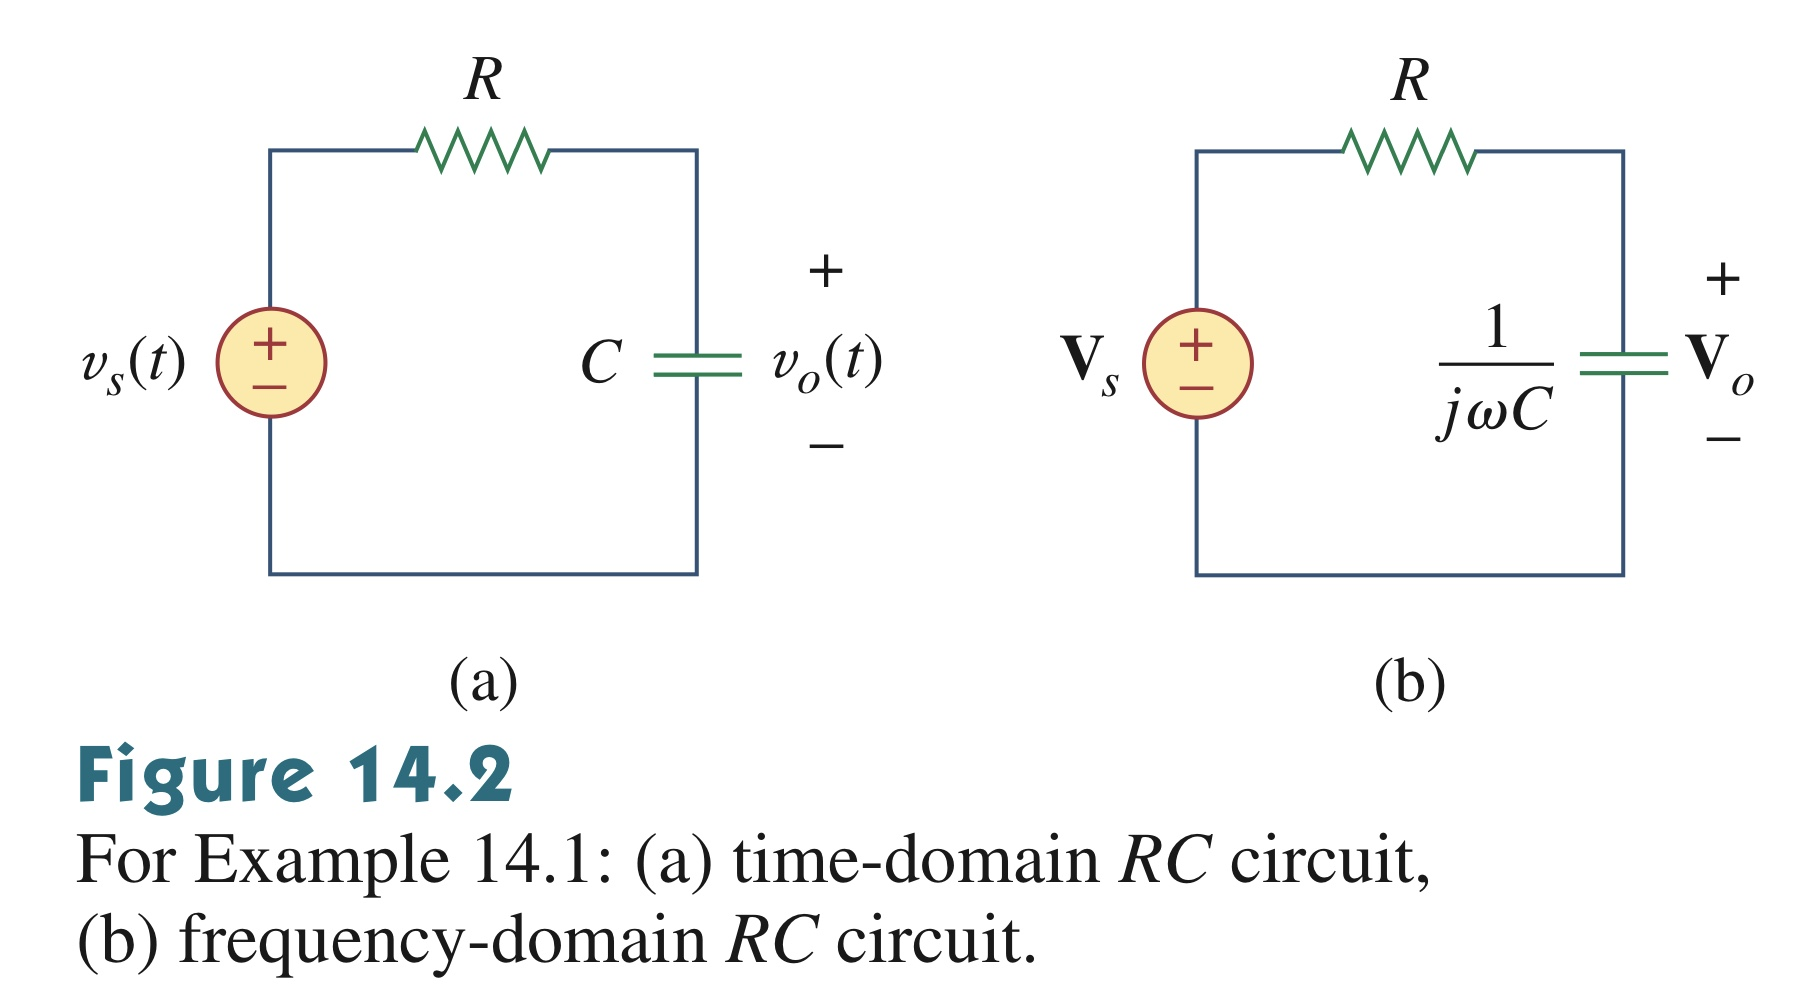
\includegraphics[width=0.6\textwidth]{C14/ex1.jpg}
    \end{figure}
\end{frame}

%%%%%%%%%%%%%%%%%%%%%%%%%

\begin{frame}{Exercise: Transfer Function}
First convert the time-domain circuit to \textbf{frequency-domain} circuit.
\newline。
\newline
Using voltage division, we obtain transfer function:
$$\textbf{\mathrm{H}}(\omega)=\dfrac{V_o}{V_s}=\dfrac{1/j\omega C}{R+1/j \omega C}=\dfrac{1}{1+j \omega RC}$$
\newline
Then we obtain the magnitude and phase
$$H=\dfrac{1}{\sqrt{1+(\omega / \omega_{0})^{2}}},\ \ \ \phi=-tan^{-1}\dfrac{\omega}{\omega_{0}}$$
where $\omega_{0}=1/RC$
\end{frame}

%%%%%%%%%%%%%%%%%%%%%%%%%
\begin{frame}{Exercise: Transfer Function}
Find the transfer function $\textbf{\mathrm{H}}(\omega)=V_{o}/V_{i}$ of the circuits below.
\begin{figure}[H]
        \centering
        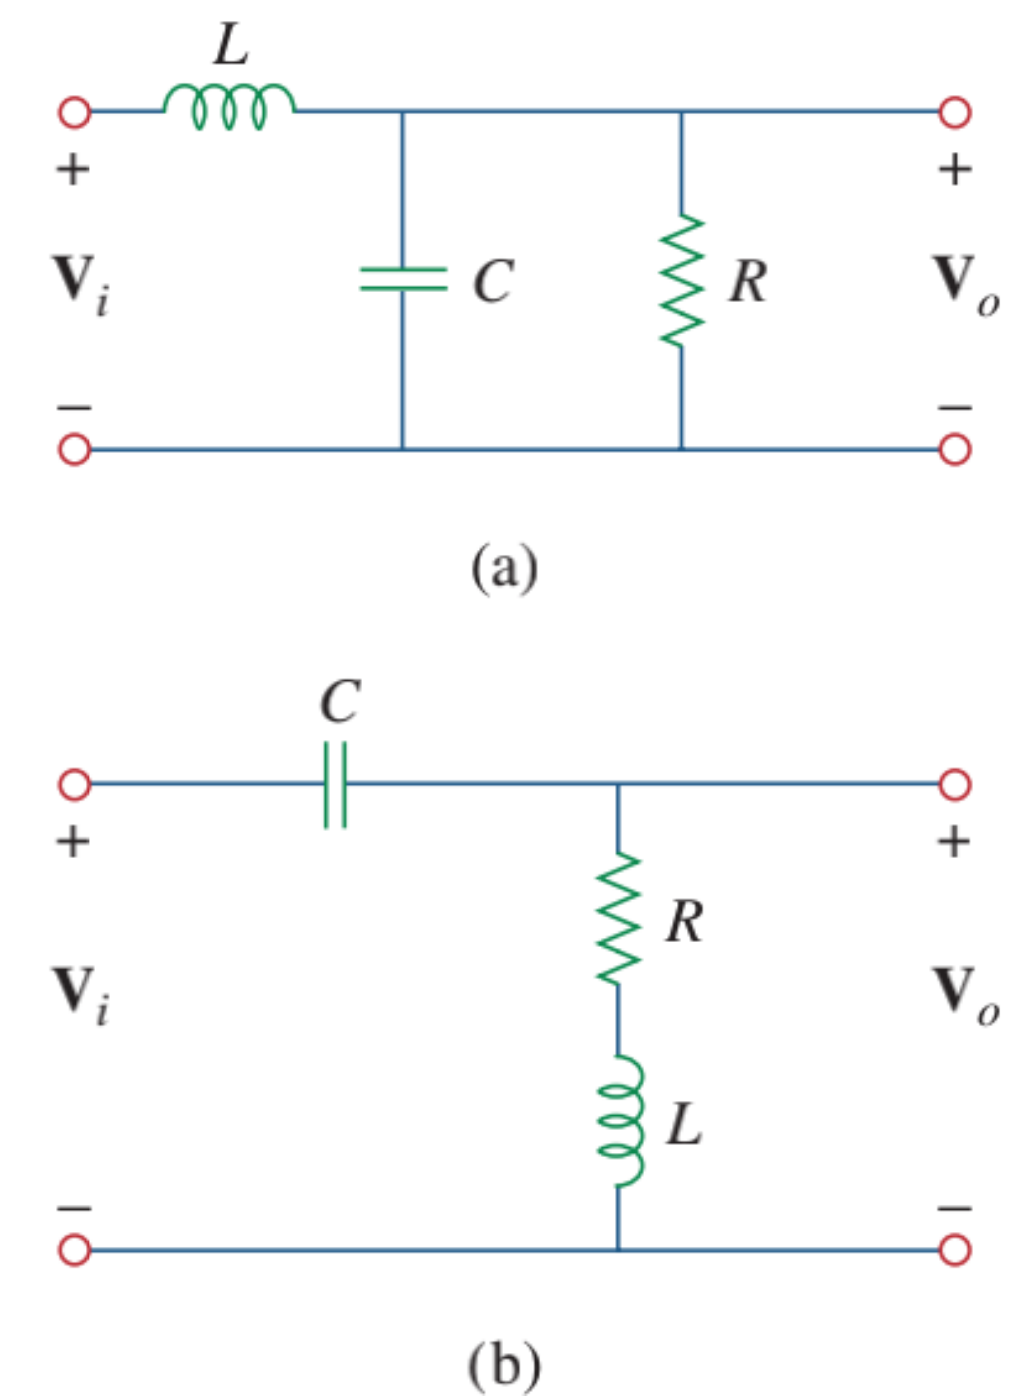
\includegraphics[width=0.4\textwidth]{C14/ex2.png}
    \end{figure}
\end{frame}

%%%%%%%%%%%%%%%%%%%%%%%%%
\begin{frame}{Exercise: Transfer Function}
A.
\newline
$R\vert \vert \frac{1}{j \omega C}=\frac{R}{1+j \omega RC}$
$\textbf{\mathrm{H}}(\omega)=\dfrac{V_{o}}{V_{i}}=\dfrac{R/(1+j \omega RC)}{j \omega L+R/(1+j \omega RC)}=\dfrac{R}{- \omega^{2}RLC+R+j\omega L}$
\newline
B.
\newline
$\textbf{\mathrm{H}}(\omega)=\dfrac{V_{o}}{V_{i}}=\dfrac{R+j \omega L}{R+j \omega L+1/j \omega C}=\dfrac{- \omega^{2}LC+j \omega RC}{1-\omega^{2}LC+j \omega RC}$
\end{frame}


%%%%%%%%%%%%%%%%%%%%%%%%%

\begin{frame}{Bode Plots}

$\mathbf{H}(\omega)$ is definitely a complex number $\mathbf{H}(\omega)=H(\omega) \angle \phi (\omega)$, and can be written as
$\mathrm{ln} \textbf{\mathrm{H}}=\mathrm{ln}H+j\phi$. The real part is a function of the magnitude while the imaginary part is the phase. So we can analyze its magnitude and phase separately, i.e.
\begin{itemize}
    \item $ H(\omega) $: magnitude frequency response
    \item $\phi (\omega)$: phase frequency response
\end{itemize}
by drawing the approximated diagrams of $H-\omega$ and $\phi-\omega$, respectively. This paired plots are so-called \textbf{Bode plots}.

\vspace{0.3cm}
\noalign \hline
\vspace{0.3cm}
For convenience, the Bode magnitude plot $H - \omega$ uses decibels for the vertical axis,
$$H_{dB} = 20\log_{10}H$$

\end{frame}

%%%%%%%%%%%%%%%%%%%%%%%%%

\begin{frame}{Bode Plots}

To draw a bode plot:

\vspace{0.3cm}

\textbf{Step 1} \ Write the targeted transfer function as the standard form
$$\mathbf{H}(\omega) = \frac{ K(j\omega)^{\pm1}(1+j\omega/z_1)(1+j2\zeta_1\omega/\omega_k+(j\omega/\omega_k)^2)\cdots }{ (1+j\omega/p_1)(1+j2\zeta_2\omega/\omega_n + (j\omega/\omega_n)^2) \cdots } $$

Then we will identify these kinds of factors:


\begin{enumerate}
\item gain/constant term: $K$
\item zero/pole at the origin: $(j \omega)^{N}$ or $\dfrac{1}{(j \omega)^{N}}$
\item simple zero/pole: $(1+j \omega /z)^{N}$ or $\dfrac{1}{(1+j \omega /p)^{N}}$
\item quadratic zero/pole: $[1+\dfrac{2j \omega \zeta}{\omega _n}+ (\dfrac{j \omega}{\omega _n})^{2}]^{N}$ or $\dfrac{1}{[1+2j \omega \zeta/\omega_{n}+(j \omega / \omega _{n})^{2} ]^{N}}$
\end{enumerate}

\end{frame}

%%%%%%%%%%%%%%%%%%%%%%%%%

\begin{frame}{Bode Plots}


\textbf{Step 2} \ Following the summary table, superpose the plots for every factor of $\mathbf{H}(\omega)$, to obtain the magnitude plot

\textbf{Step 3} \ Following the summary table, superpose the plots for every factor of $\mathbf{H}(\omega)$, to obtain the phase plot

\begin{figure}[H]
    \centering
    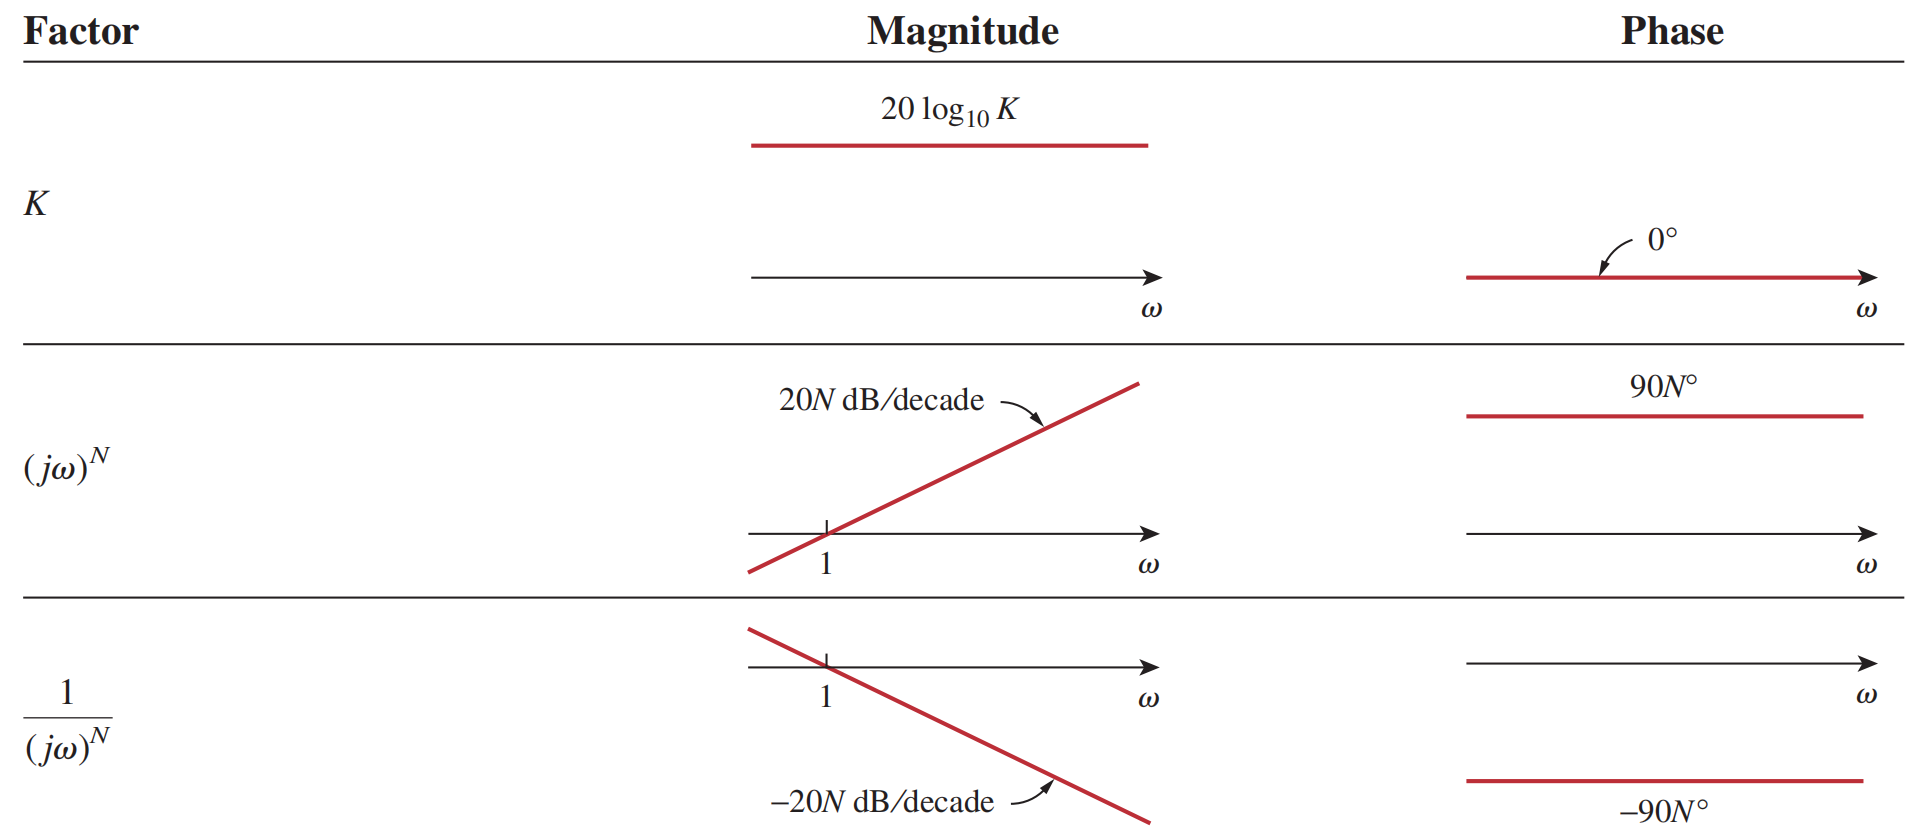
\includegraphics[width=\textwidth]{C14/bode1.png}
\end{figure}
    
\end{frame}

%%%%%%%%%%%%%%%%%%%%%%%%%

\begin{frame}{Bode Plots}
\begin{figure}[H]
    \centering
    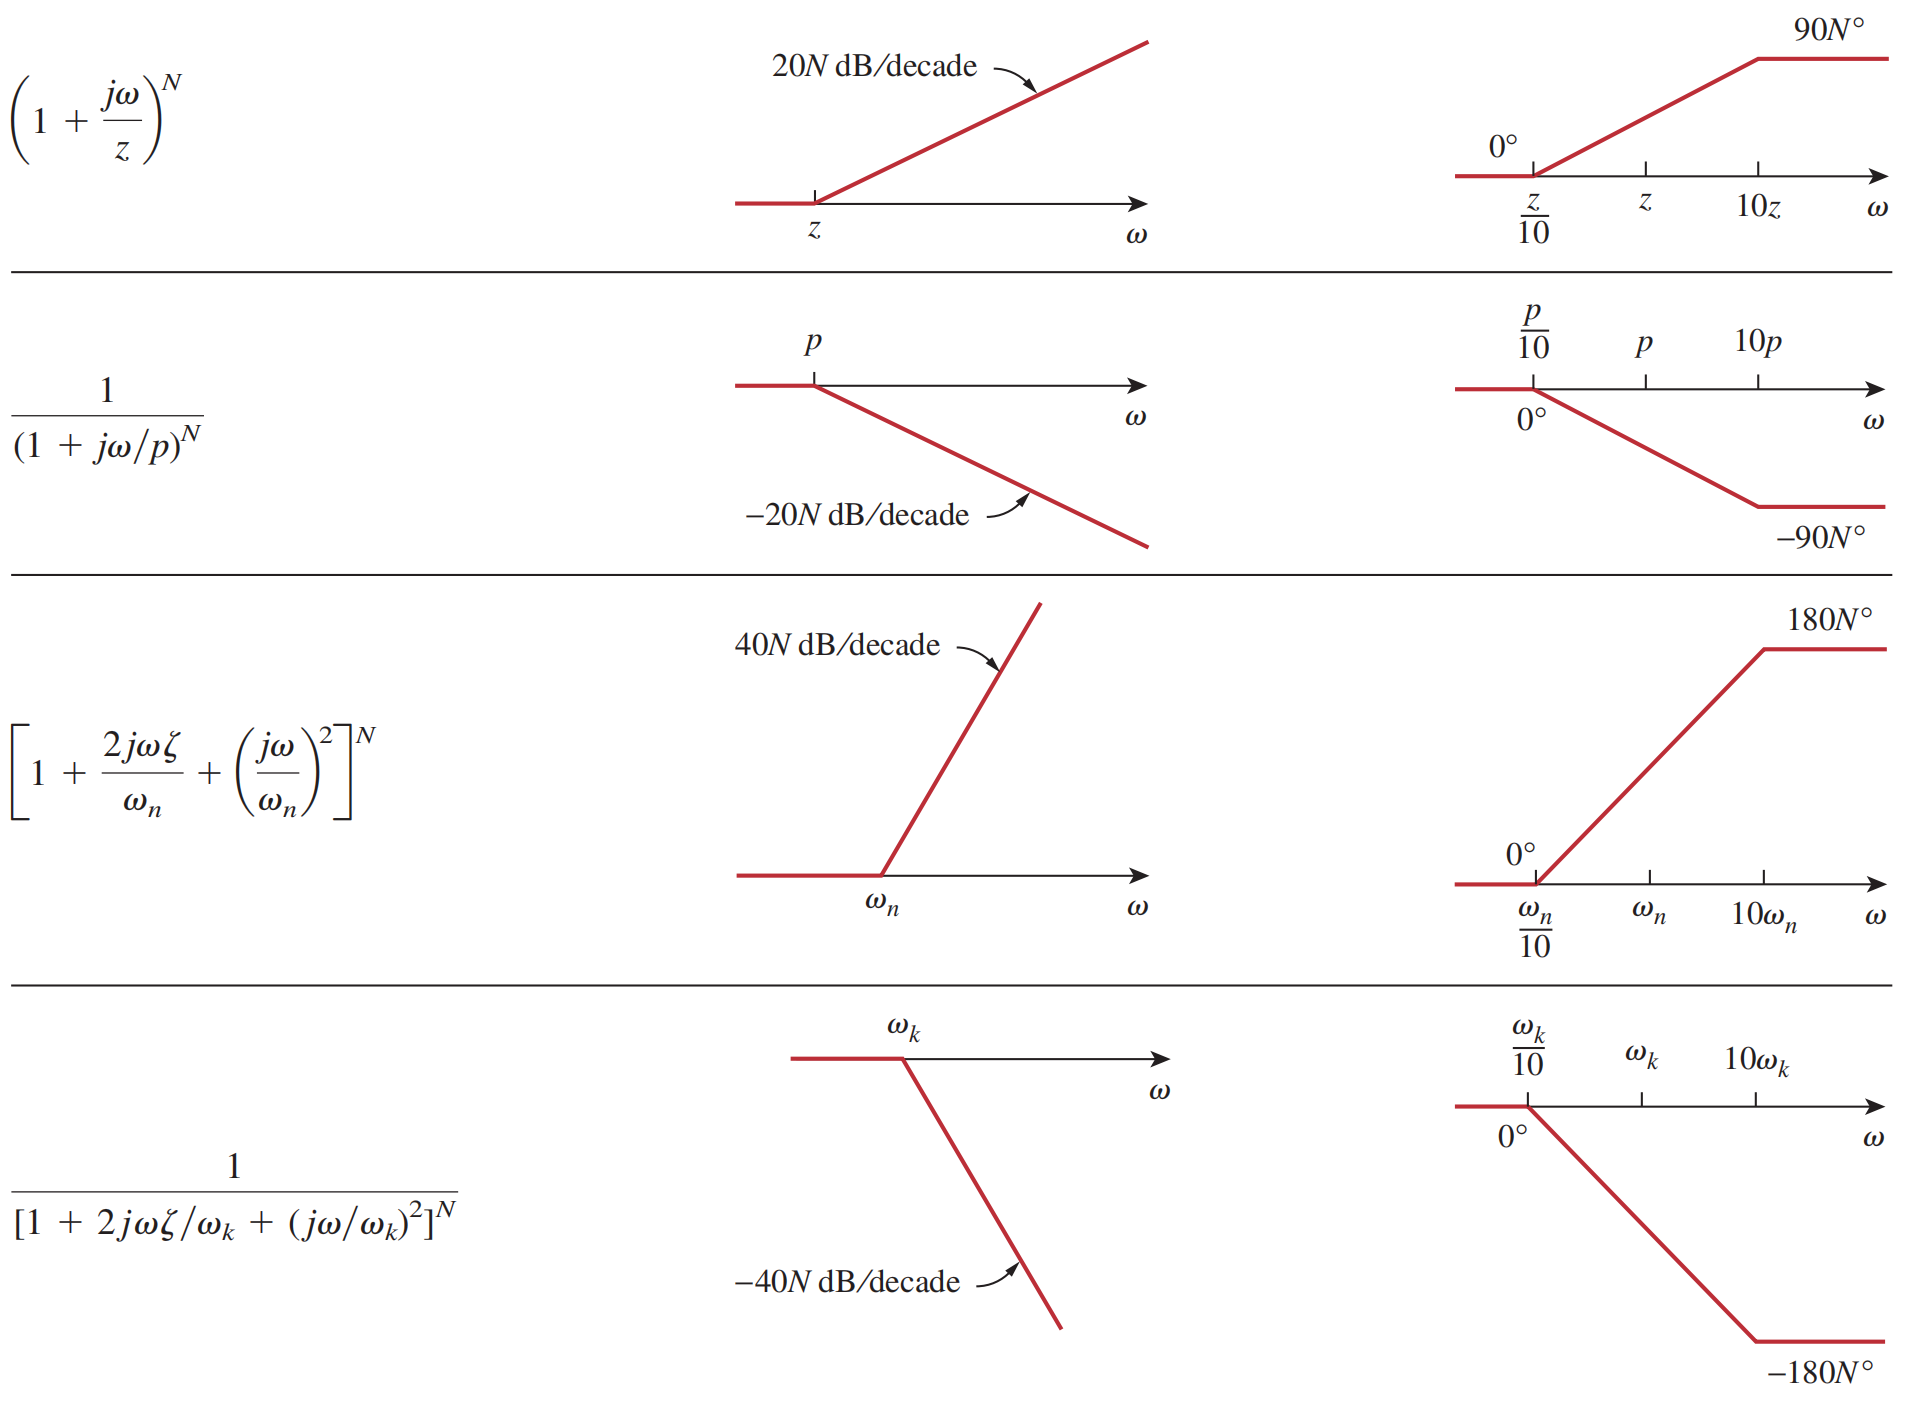
\includegraphics[width=\textwidth]{C14/bode2.png}
\end{figure}
\end{frame}



%%%%%%%%%%%%%%%%%%%%%%%%%

\begin{frame}{Bode Plots}
\textbf{Tips on Summary Table}:
\begin{itemize}
\item zeros: upward turn
\item poles: downward turn
\item for the factor constant K, be careful with the phase angle.
$$\phi=
\begin{cases}
0^{\circ}& \text{K\textgreater 0}\\
\pm 180^{\circ}& \text{K\textless 0}
\end{cases}$$
\item Be careful with $N$. It influences the slope.
\item for simple/quadratic poles/zeros: straight-line approximation
\item for quadratic poles/zeros: can be treated as a double pole/zero
\begin{figure}[H]
        \centering
        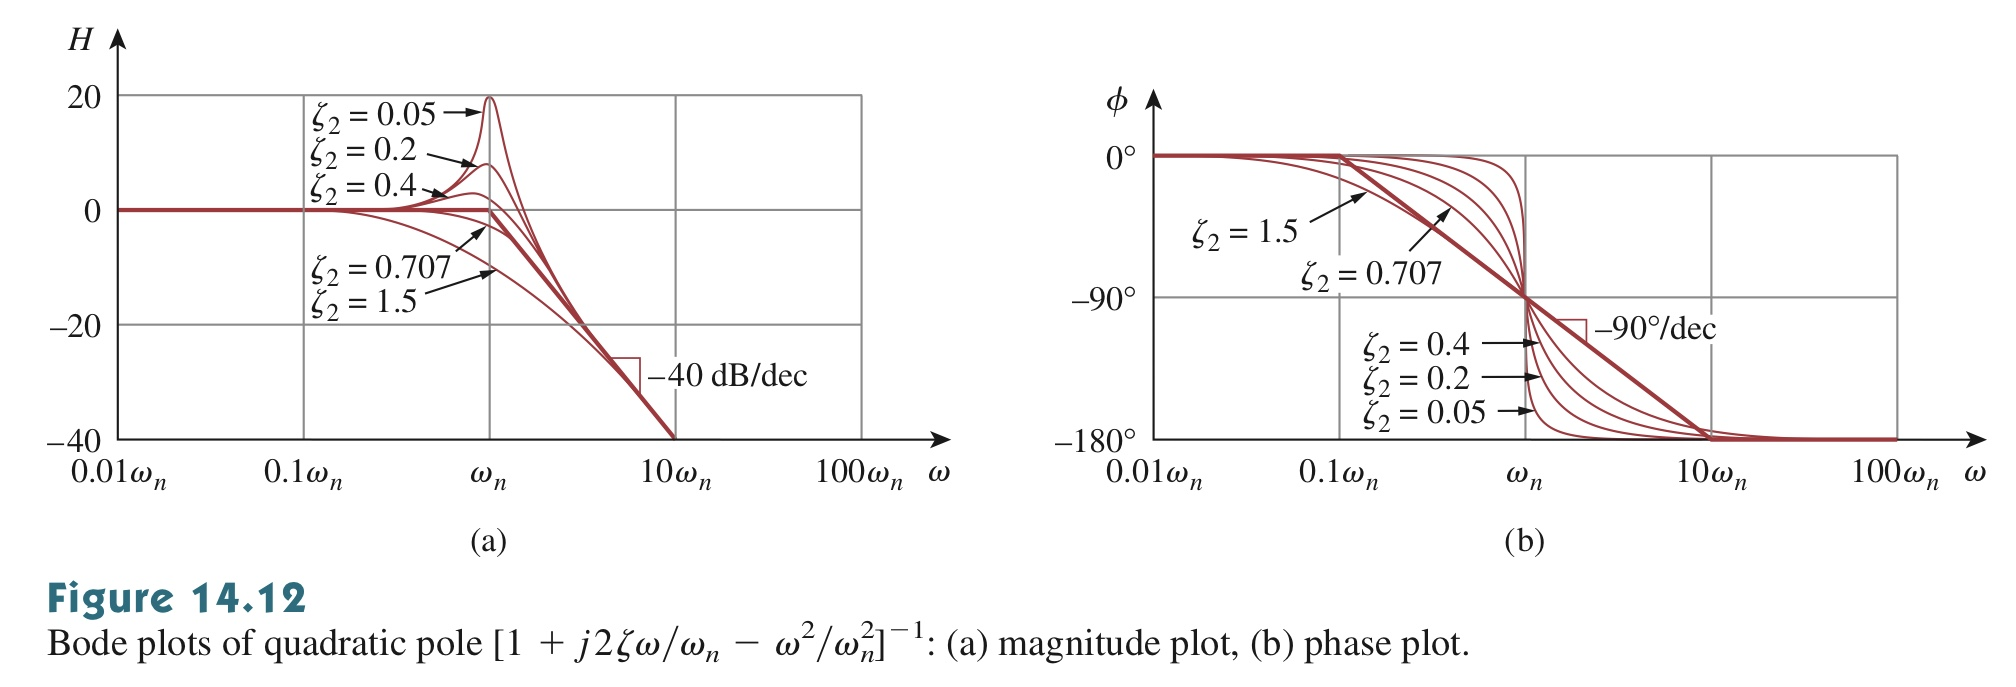
\includegraphics[width=0.5\textwidth]{C14/quadratic.jpg}
    \end{figure}
\end{itemize}
\end{frame}

%%%%%%%%%%%%%%%%%%%%%%%%%

\begin{frame}{Bode Plots}

\textbf{Steps}:
\begin{enumerate}
\item Convert the transfer function to the standard form.
\item Get equation of magnitude and phase. (optional)
\item Use the summary table to sketch magnitude and phase plots. 
\begin{itemize}
\item dotted lines for each factor
\item solid line for final result
\end{itemize}
\end{enumerate}

\textbf{Label}:
\begin{itemize}
\item x-label
\item slope / $H_{dB}$ and $\phi$ coordinate label
\end{itemize}
\end{frame}


%%%%%%%%%%%%%%%%%%%%%%%%%

\begin{frame}{Exercise: Bode Plots}

Draw the bode plots of
$$\mathbf{H}(\omega)=\dfrac{200j \omega}{(j \omega+2)(j \omega+10)}$$

\end{frame}

%%%%%%%%%%%%%%%%%%%%%%%%%

\begin{frame}{Exercise: Bode Plots}

First, write it in the standard form:
\begin{equation*}
\begin{aligned}
\mathrm{H}(\omega)&=\dfrac{10j \omega}{(1+j \omega /2)(1+j \omega/10)}\\
&=\dfrac{10\lvert j \omega \rvert}{\lvert 1+j \omega /2 \rvert \lvert 1+j \omega/10 \rvert} \angle 90^{\circ}-\mathrm{tan}^{-1}\omega /2-\mathrm{tan}^{-1}\omega /10
\end{aligned}
\end{equation*}
Hence, the magnitude and phase are:
\begin{equation*}
\begin{aligned}
H_{dB}&=20 \mathrm{log}_{10}10+20\mathrm{log}_{10} \lvert j \omega \rvert -20 \mathrm{log}_{10} \lvert 1+ \dfrac{j \omega}{2} \rvert-20\mathrm{log}_{10} \lvert 1+\dfrac{j \omega}{10} \rvert\\
\phi &=90^{\circ}-\mathrm{tan}^{-1}\dfrac{\omega}{2}-\mathrm{tan}^{-1}\dfrac{\omega}{10}
\end{aligned}
\end{equation*}
\end{frame}

%%%%%%%%%%%%%%%%%%%%%%%%%

\begin{frame}
\frametitle{Exercise: Bode Plots}
\begin{figure}[H]
        \centering
        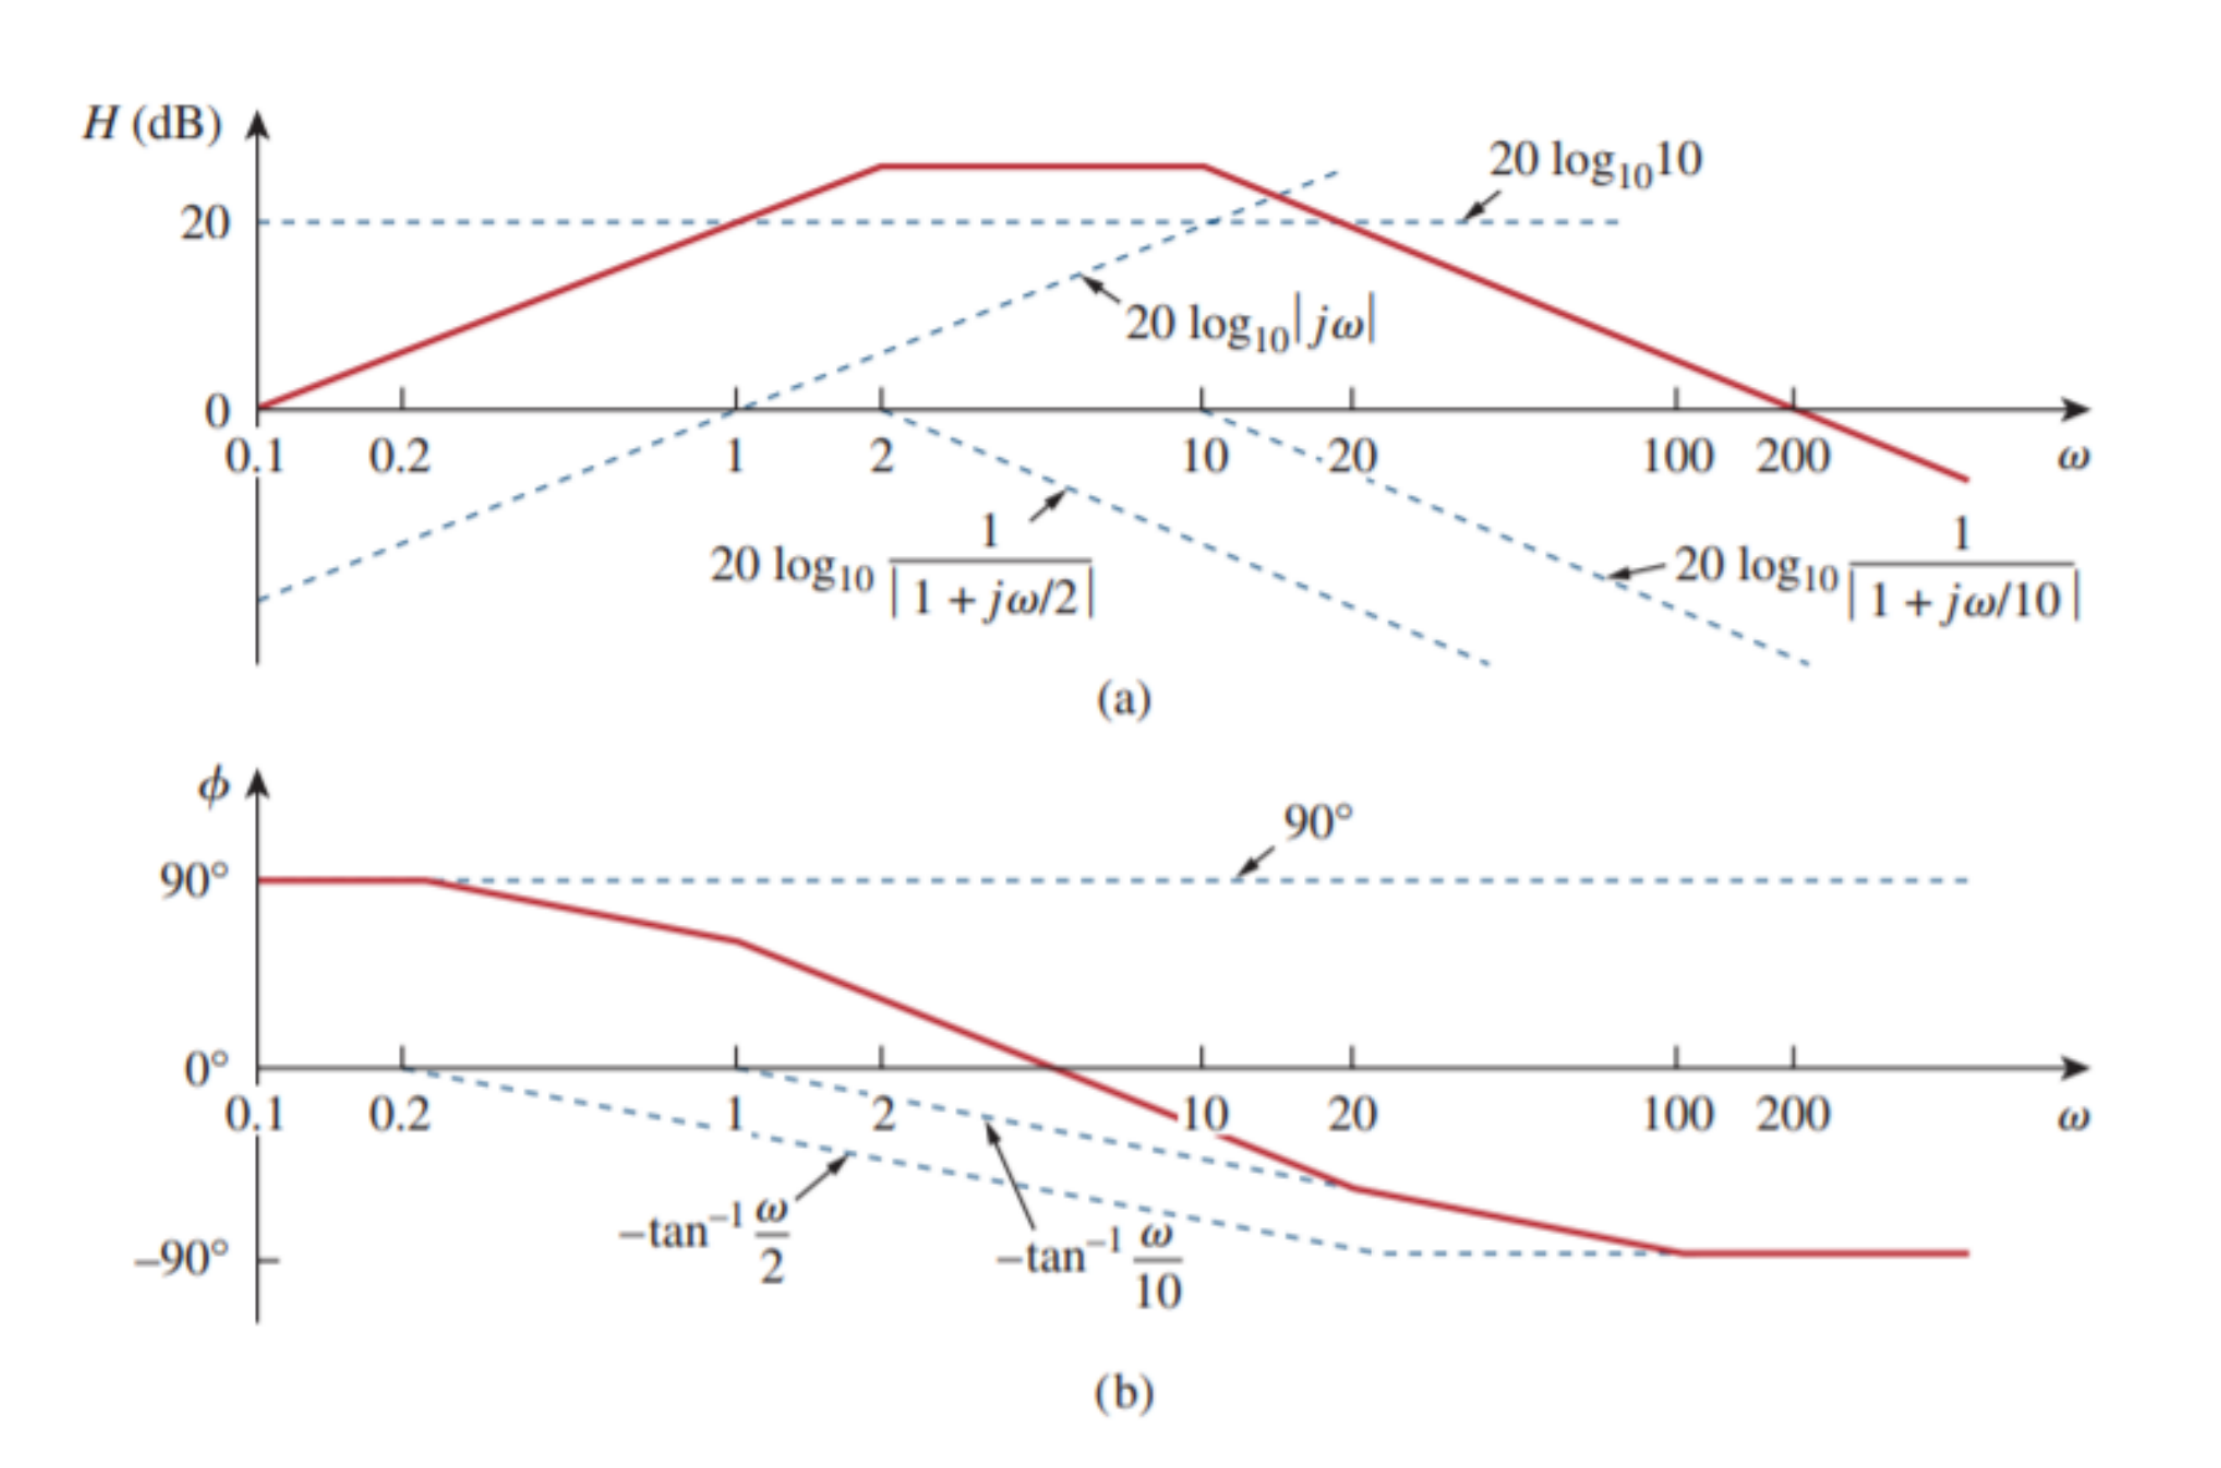
\includegraphics[width=0.95\textwidth]{C14/a3.png}
    \end{figure}
\end{frame}

%%%%%%%%%%%%%%%%%%%%%%%%%

\begin{frame}{Resonance}

\textbf{Resonance} happens in an RLC circuit (series or parallel), when the capacitive and inductive reactances of the circuit are equal. When resonance happens,
\begin{itemize}
    \item The total impedance is purely resistive, $\mathrm{Im}(Z)=0$.
    \item Source voltage $\mathbf{V}$ and current $\mathbf{I}$ are in phase.
    \item The magnitude of current, $\vert \mathbf{I}\vert$, is maximum. 

        (since $\vert \mathbf{Z}\vert$ is minimum in $\vert \mathbf{I}\vert = \frac{\vert \mathbf{V}\vert}{\vert \mathbf{Z}\vert}$)
    \item The power $P$ dissipated on the load is maximum.

        (since $P = \vert \mathbf{I}\vert ^2R$)
\end{itemize}

With a given RLC circuit, our main interest is to find the frequency $\omega_0$ to achieve the resonance condition.

    
\end{frame}

%%%%%%%%%%%%%%%%%%%%%%%%%

\begin{frame}{Resonance}

\begin{itemize}
    \item $Q$: quality factor, a measure of the circuit's energy storage capacity
    \item $\omega_1, \omega_2$: half-power frequencies, the frequencies at which the power dissipated is half of the maximum
    \item $B = \omega_2 - \omega_1$: bandwidth
\end{itemize}

\begin{table}[]
    \centering
    \begin{tabular}{ccc}
        \toprule
       & Series RLC & Parallel RLC \\
       \midrule
       Diagram & 
       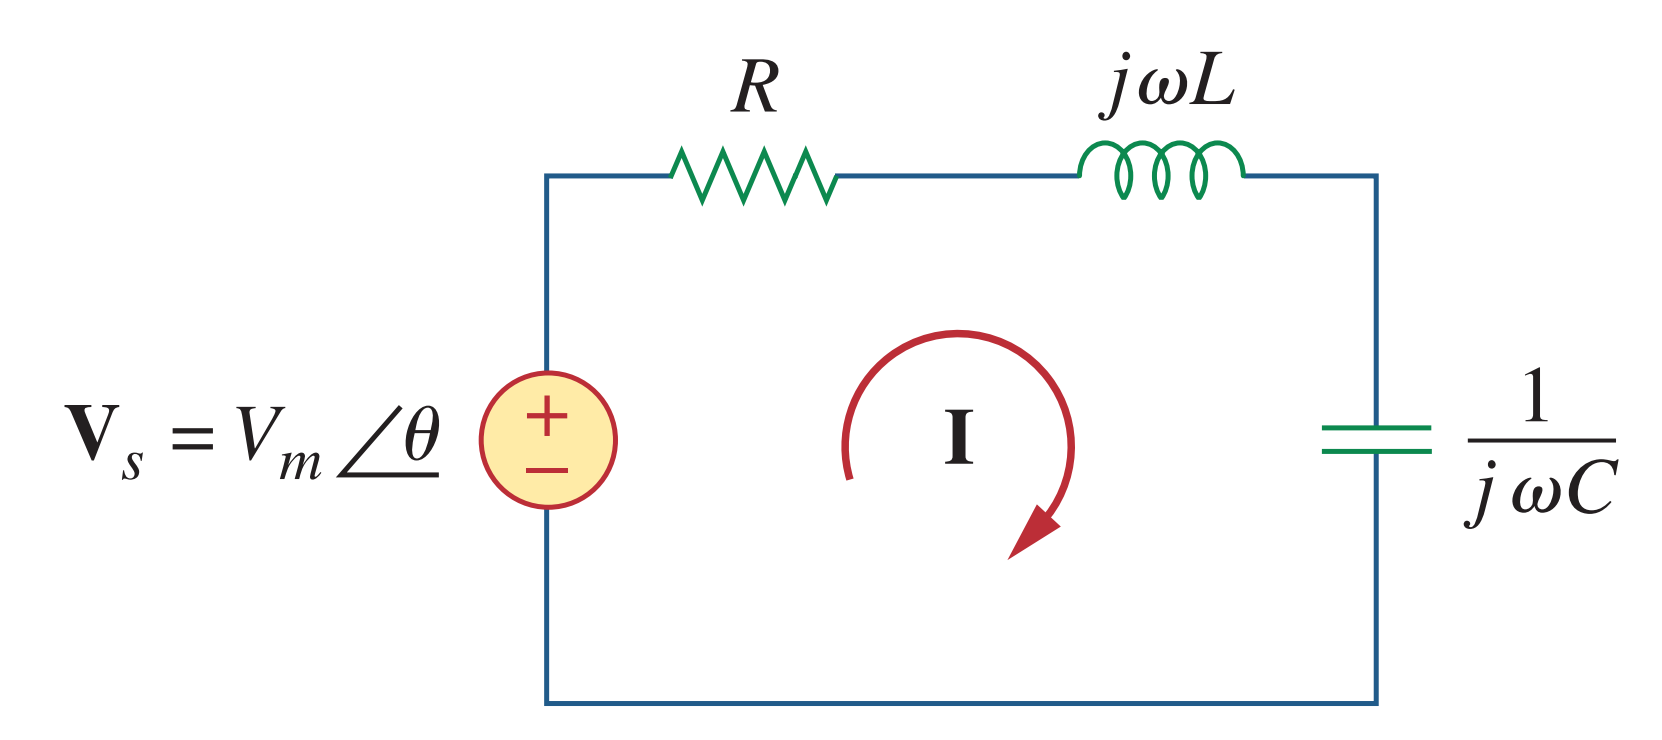
\includegraphics[width=0.4\textwidth]{C14/resonance1.png}
       & 
       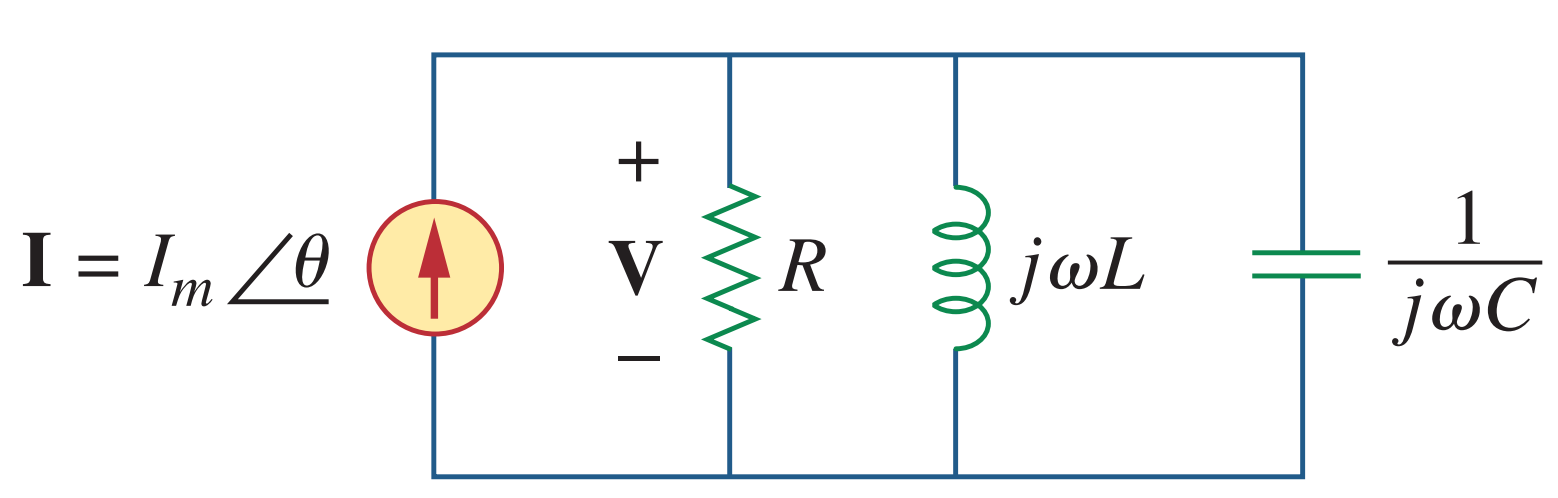
\includegraphics[width=0.4\textwidth]{C14/resonance2.png}
       \\
        $\omega_0$ & $1/\sqrt{LC}$ & $1/\sqrt{LC}$ \\
        $Q$ & $=\frac{\omega_0L}{R}=\frac{1}{\omega_0RC}$ & $=\frac{R}{\omega_0L}=\omega_0RC$ \\
        $B$ & $\omega_0/Q$ & $\omega_0/Q$ \\
        $\omega_1, \omega_2$ & $\omega_0 \sqrt{1+(\frac{1}{2Q})^2} \pm \omega_0/2Q$ & $\omega_0 \sqrt{1+(\frac{1}{2Q})^2} \pm \omega_0/2Q$ \\
        \bottomrule
    \end{tabular}
\end{table}
    
\end{frame}

%%%%%%%%%%%%%%%%%%%%%%%%%

\begin{frame}{Filters}
A \textbf{filter} is a circuit that pass signals with desired frequencies and reject others.

\begin{small}
    (There is no need to know too much about the mechanism of filters in VE215. It is a topic of VE216. In this section, memorizing various types of filters and their formulas is enough.)
\end{small}

\vspace{0.5cm}

Two types of filters
\begin{itemize}
    \item Passive filters (built with RC or RLC circuit)
    \item Active filters (built with R + C + op-amp)
\end{itemize}


\end{frame}


%%%%%%%%%%%%%%%%%%%%%%%%%

\begin{frame}{Filters: Passive Filters}

\begin{table}[]
    \centering
    \begin{tabular}{cc}
        \toprule
        \textbf{Lowpass filter} & \textbf{Highpass filter}  \\
        \midrule
        \includegraphics[width=0.4\textwidth]{C14/lowpass_diagram.jpeg}
         &
         \includegraphics[width=0.4\textwidth]{C14/highpass_diagram.jpeg}
         \\
        \includegraphics[width=0.4\textwidth]{C14/lowpass.jpeg}
        & 
        \includegraphics[width=0.4\textwidth]{C14/highpass.jpeg}
        \\
        $\omega_c = 1/RC$ & $\omega_c = 1/RC$ \\
        \bottomrule
    \end{tabular}
\end{table}

Their difference is on where the output is connected across.
    
\end{frame}

%%%%%%%%%%%%%%%%%%%%%%%%%

\begin{frame}{Filters: Passive Filters}

\begin{table}[]
    \centering
    \begin{tabular}{cc}
        \toprule
        \textbf{Bandpass filter} & \textbf{Bandstop filter}  \\
        \midrule
        \includegraphics[width=0.4\textwidth]{C14/bandpass_diagram.jpeg}
         &
         \includegraphics[width=0.4\textwidth]{C14/bandstao_diagram.jpeg}
         \\
        \includegraphics[width=0.4\textwidth]{C14/bandpass.jpeg}
        & 
        \includegraphics[width=0.4\textwidth]{C14/bandstop.jpeg}
        \\
        $\omega_0 = 1/\sqrt{LC}$ & $\omega_c = 1/\sqrt{LC}$ \\
        \bottomrule
    \end{tabular}
\end{table}

Their difference is on where the output is connected across.

\end{frame}

%%%%%%%%%%%%%%%%%%%%%%%%%

\begin{frame}{Filters: Active filters}

\begin{table}[]
    \centering
    \begin{tabular}{cc}
        \toprule
        \textbf{1st-order lowpass filter} & \textbf{1st-order highpass filter}  \\
        \midrule
        \includegraphics[width=0.4\textwidth]{C14/active_lowpass.jpeg}
        & 
        \includegraphics[width=0.4\textwidth]{C14/active_highpass.jpeg}
        \\
        $\omega_c = 1/R_fC_f$ & $\omega_c = 1/R_iC_i$ \\
        \bottomrule
    \end{tabular}
\end{table}
    
\end{frame}

%%%%%%%%%%%%%%%%%%%%%%%%%

\begin{frame}{Filters: Active filters}

\begin{figure}
    \centering
    \includegraphics[width=0.9\textwidth]{C14/active_bandpass.jpeg}
\end{figure}

$$\omega_1 = 1/RC_1, \omega_2 = 1/RC_2$$

\end{frame}


%%%%%%%%%%%%%%%%%%%%%%%%%%%%%%%%%%%%%%%%%%%%%%%%%%%
\begin{frame}
\frametitle{References}
\begin{enumerate}
\item 2023 Summer VE215 slides, Rui Yang
\item Fundamentals of Electric Circuits, 5th e, Sadiku, Matthew
\item 2022 Fall VE215 Final RC, Zhiyu Zhou, Yuxuan Peng, Yifei Cai
\end{enumerate}
\end{frame}


\begin{frame}
\huge{\centerline{Good luck on your final exam!}}
\end{frame}


\end{document}
